% IACR Transactions CLASS DOCUMENTATION
% Written by Gaetan Leurent gaetan.leurent@inria.fr (2016-2018)
%
% To the extent possible under law, the author(s) have dedicated all
% copyright and related and neighboring rights to this software to the
% public domain worldwide. This software is distributed without any
% warranty.
%
% You should have received a copy of the CC0 Public Domain Dedication
% along with this software. If not, see
% <http://creativecommons.org/publicdomain/zero/1.0/>.

\documentclass{iacrtrans}
\usepackage[utf8]{inputenc}
% *** MATH PACKAGES ***
%
\usepackage{amsmath}
\usepackage{listings}% use mathematical symbols in Verbatim environment
\lstset{
  basicstyle=\ttfamily,
  mathescape
}
\usepackage{amsfonts,amssymb}
\usepackage[linesnumbered,boxed,vlined]{algorithm2e}
% *** ALIGNMENT PACKAGES ***
%
\usepackage{array}
% *** PDF, URL AND HYPERLINK PACKAGES ***
%
\usepackage{url}



%personal defined packages
\usepackage{multirow,array}
% *** TABLE FOOTNOTE PACKAGES ***
\usepackage[bottom]{footmisc}
\usepackage{footnote}
\makeatletter
\def\@xfootnote[#1]{%
  \protected@xdef\@thefnmark{#1}%
  \@footnotemark\@footnotetext}
\makeatother
\usepackage{threeparttable}
\usepackage{diagbox}

\usepackage{caption}
\usepackage{subcaption}

\usepackage{placeins}

 %table dash line
% \usepackage{arydshln}

% \usepackage{morefloats}

% \usepackage{fancyvrb}
% \usepackage{xcolor}

% align center vertically in table
\newcolumntype{L}[1]{>{\raggedright\arraybackslash}m{#1}}
\newcolumntype{C}[1]{>{\centering\arraybackslash}m{#1}}
\newcolumntype{R}[1]{>{\raggedleft\arraybackslash}m{#1}}

\newcommand{\tabincell}[2]{\begin{tabular}{@{}#1@{}}#2\end{tabular}}

\theoremstyle{plain}
\newtheorem{thm}{Theorem}[section]
\newtheorem{lem}[thm]{Lemma}
\newtheorem{prop}[thm]{Proposition}
\newtheorem*{cor}{Corollary}

\usepackage{makecell}

\author{Jingwei Hu\inst{1} \and Unknown\inst{2}}
\institute{Nanyang Technological University, Singapore, \email{davidhu@ntu.edu.sg} \and
           Unknown}
\title[]{Number-Theoretic Transform Architecture for Fully Homomorphic Encryption from Hypercube Topology}
\subtitle{}

\begin{document}

\maketitle

% use optional argument because the \LaTeX command breaks the PDF keywords
\keywords{Fully Homomorphic Encryption, Number Theoretic Transform, FPGA Implementation}

\begin{abstract}
This paper introduces a high-performance and scalable hardware architecture designed for the Number-Theoretic Transform (NTT), a fundamental component extensively utilized in lattice-based encryption and fully homomorphic encryption schemes.

The underlying rationale behind this research is to harness the advantages of the hypercube topology. This topology serves to significantly diminish the volume of data exchanges required during each iteration of the NTT, reducing it to a complexity of $\Omega(\log N)$. Concurrently, it enables the parallelization of $N$ processing elements. This reduction in data exchange operations is of paramount importance. It not only facilitates the establishment of interconnections among the $N$ processing elements but also lays the foundation for the development of a high-performance NTT design. This is particularly valuable when dealing with large values of $N$.
\end{abstract}
\newpage
\tableofcontents{}
\newpage

\section*{Introduction}

The contributions of this paper include:
\begin{itemize}
    \item Pioneering Hypercube Topology in NTT Designs: This research introduces the innovative concept of applying hypercube topology to NTT designs. It successfully addresses the challenging issue of managing a substantial volume of data exchange within high-performance NTT designs.
    \item Prototyping a Hypercube-Based NTT Hardware: The study provides a practical implementation of NTT hardware based on the hypercube topology. Importantly, it allows users the flexibility to configure the degree of parallelization as per their requirements. The paper also offers theoretical estimations of the timing performance, which are subsequently validated through concrete implementation results.
\end{itemize}


\section{FHEW-like Fully Homomorphic Encryption Scheme}

\section{Number-theoretic transform with merged twiddle factors}
This section describes NTT hardware at the bottom level. Firstly,  The distinguishing feature is that a series of new twiddle factor LUTs  is constructed and used:  an independent twiddle factor LUT, denoted as $\{w_i[\cdot]\}_{i=0,\ldots,log_2N-1}$, is prepared for the $i$-th round of butterfly computation ($logN$ rounds in total) as described in Alg.~\ref{alg:descript_twiddlefactor}. Note that differing from the standard FFT which uses twiddle factor $\omega_{N}^i$ for $i\in [N]$, the NTT used in the ring $\mathcal{R}_q$ uses the modified twiddle factor $\omega_N^i\cdot\omega_{2N}^j$ for $i\in [N], j=2^0,2^1,\cdots,2^{logN-1}$.

\subsection{Higher level description for NTT with merged twiddle factors}\label{sec:gf2m_arith}

In this subsection, we discuss the NTT algorithm with merged twiddle factors. No pre-processing or post-processing is required in this variant of NTT algorithm. At an abstract level, the structure of this NTT algorithm is identical to that of the classic FFT algorithm. 


The formal description of this NTT variant is shown in Alg.~\ref{alg:descript_ntt} which is also refered to as Cooley-Tukey (CT) butterfly or decimation in time (DIT) in the open literature. It is essentially identical to the classic FFT algorithm except the twiddle factor array $w_i[\cdot]$. It has $logN$ iterations (loop-$i$) at outermost, where each iteration computes one layer of butterfly computations.  The $i(i=0,\cdots,logN-1)$-th layer of butterfly computation always has $\frac{N}{2}$ butterflies. These butterflies are bundled into $2^i$ groups (recorded by the variable $NumberofGroups$) and each groups has $\frac{N}{2^i}$ pairs of butterflies (recorded by the variable $PairsInGroup$). The key feature is that at a particular iteration (say the $i$-th iteration), the butterflies in a particular group (say the $k$-th group) share the same twiddle factor $w_i[k]$. The variable $Distance$ is used to locate precisely two inputs of a particular pair of butterfly in loop-$j$, \textit{i.e.}, $a[j]$ and $a[j+Distance]$. The variables $JFirst$ and $JLast$ indicate the starting and the ending position of the array $a[\cdot]$, respectively, used in the $k$-th group of the $i$-th iteration.

A visualization of Alg.~\ref{alg:descript_ntt} is depicted in Fig.~\ref{fig:dit1} when $N=8$. The inputs are $a[0],\cdots,a[7]$ where $a[i]$ represents the $i$-th coefficient $a_i$ in the polynomial $a(X)=\sum_{i=0}^{N-1}a_iX^i$. The NTT computation has 3 layers of butterflies: In the first layer ($i=0$ for loop-$i$ in Alg.~\ref{alg:descript_ntt}), only one butterfly group (associated with twiddle factor $\omega_{16}^4$) exists; in the second layer, two butterfly groups (associated with twiddle factor $\omega_{16}^2$ and $\omega_{16}^6$) exist; in the third layer, four butterfly groups (associated with twiddle factors $\omega_{16}^1$, $\omega_{16}^5$, $\omega_{16}^3$, and $\omega_{16}^7$, respectively) exist. It is worth noting that the ouputs from the NTT network is in bit-reversed order as $A[0],A[4],A[2],A[6],A[1],A[5],A[3],A[7]$.

\begin{algorithm}[!tbh]
 \DontPrintSemicolon % Some LaTeX compilers require you to use \dontprintsemicolon instead
 \KwIn{polynomial $a(x)\in R_q$ represented in an array {}$a[\cdot]$, Twiddle factors $\{w_i[\cdot]\}_{i=0,\ldots,log_2N-1}$}
 \KwOut{NTT($a(x)$) represented in $a[\cdot]$ (in-place)}
    $PairsInGroup \gets N/2$\;
    $NumOfGroups \gets 1$\;
    $Distance \gets N/2$\;
    \For{$i\leftarrow 0$ \KwTo $log_2N-1$}{
        \For{$k\leftarrow 0$ \KwTo $NumOfGroups-1$}{
            $JFirst \gets 2\cdot k \cdot PairsInGroup$\;
            $JLast \gets JFirst + PairsInGroup-1$\;
            \For{$j\leftarrow JFirst$ \KwTo $JLast$}{
                $Temp \gets w_i[k]*a[j+Distance]$\;
                $a[j+Distance] \gets a[j]-Temp$\;
                $a[j] \gets a[j] + Temp$\;
            }             
        }      
        $PairsInGroup \gets PairsInGroup/2$\;
        $NumOfGroups \gets NumOfGroups\cdot 2$\;
        $Distance \gets Distance/2$\;
    }
    \Return {$a[\cdot]$\;}
 \caption{Higher level description of NTT, \textit{a.k.a} $DIT_{NN\to RN}$}\label{alg:descript_ntt}
\end{algorithm}

\begin{algorithm}[!tbh]
 \DontPrintSemicolon % Some LaTeX compilers require you to use \dontprintsemicolon instead
 \KwIn{a polynomial ring $R_q$, and NTT points $N$}
 \KwOut{Twiddle factors $\{w_i[\cdot]\}_{i=0,\ldots,log_2N-1}$ used in Algorithm~\ref{alg:descript_ntt}}
    $FirstPart \gets [0\cdots0]_2$\;{}
    $SecondPart \gets [1\cdots0]_2$\;
    \For{$i\leftarrow 0$ \KwTo $log_2N-1$}{
        \For{$j\leftarrow 0$ \KwTo $N-1$}{
            $[j_{log_2N-1,\cdots,j_0}]_2 \gets BinRepr(j)$\;
            $w_i[j] \gets \phi^{Firstpart}\cdot \phi^{SecondPart}$\;         
        }   
        $FirstPart \gets RightRot(FirstPart, j_{log_2N-1-i})$\;   
        $SecondPart \gets SecondPart/2$\;
    }
    \Return {$\{w_i[\cdot]\}_{i=0,\ldots,log_2N-1}$\;}
 \caption{Construction of Twiddle Factor LUTs}\label{alg:descript_twiddlefactor}
\end{algorithm}

Next, we detail how to construct the twiddle factor LUT. Recall the NTT with pre-processing can be written together as a summation of $N$ terms:
\[
    A_i = \sum_{j=0}^{N-1}a_j\omega_{2N}^j\omega_N^{ij} \bmod q, i\in [0,N-1]
\]

Next, by splitting the summation above into even and odd groups according to the index $i$ of $A_i$, we obtain
\begin{gather}
    A_i = \sum_{j=0}^{\frac{N}{2}-1}a_{2j}\omega_N^{2ij}\omega_{2N}^{2j}  + \sum_{j=0}^{\frac{N}{2}-1}a_{2j+1}\omega_N^{i(2j+1)}\omega_{2N}^{2j+1} \bmod q \text{ for } i\in [0,\frac{N}{2}-1]\notag\\
    = \sum_{j=0}^{\frac{N}{2}-1}a_{2j}\omega_{\frac{N}{2}}^{ij}\omega_{N}^{j}  + \omega_{N}^i\omega_{2N}\sum_{j=0}^{\frac{N}{2}-1}a_{2j+1}\omega_{\frac{N}{2}}^{ij}\omega_N^{j} \bmod q \notag
\end{gather}
Now express $A_i$s into the first half $A_{i}$ and the second half $A_{i+\frac{N}{2}}$ as follows: 
\begin{gather}
    A_i = \sum_{j=0}^{\frac{N}{2}-1}a_{2j}\omega_{\frac{N}{2}}^{ij}\omega_{N}^{j}  + \omega_{N}^i\omega_{2N}\sum_{j=0}^{\frac{N}{2}-1}a_{2j+1}\omega_{\frac{N}{2}}^{ij}\omega_N^{j} \bmod q \text{ for } i\in [0,\frac{N}{2}-1]\notag\\
   A_{i+\frac{N}{2}} = \sum_{j=0}^{\frac{N}{2}-1}a_{2j}\omega_{\frac{N}{2}}^{ij}\omega_{N}^{j}  - \omega_{N}^i\omega_{2N}\sum_{j=0}^{\frac{N}{2}-1}a_{2j+1}\omega_{\frac{N}{2}}^{ij}\omega_N^{j} \bmod q \notag
\end{gather}

Assume $N=2^n$, let $Y_i^{(n-1)}$ and $Z_i^{(n-1)}$ be solutions to the two half-sized subproblems (NTT of size of $\frac{N}{2}=2^{n-1}$ for the even terms $\{a_{2j}\}_{j\in [\frac{N}{2}]}$ and the odd terms $\{a_{2j+1}\}_{j\in [\frac{N}{2}]}$) defined by
\begin{gather}
    Y_i^{(n-1)} = \sum_{j=0}^{\frac{N}{2}-1}a_{2j}\omega_{\frac{N}{2}}^{ij}\omega_{N}^{j} \bmod q \text{ for } i\in [0,\frac{N}{2}-1]\notag\\
    Z_i^{(n-1)} = \sum_{j=0}^{\frac{N}{2}-1}a_{2j+1}\omega_{\frac{N}{2}}^{ij}\omega_N^{j} \bmod q \notag
\end{gather}

Therefore, the equation above is rewritten in a more compact form:
\begin{gather}
    Y_i^{(n)} = Y_i^{(n-1)} + \omega_{N}^i\omega_{2N}\cdot Z_i^{(n-1)} = A_i\bmod q \text{ for } i\in [0,\frac{N}{2}-1]\notag\\
    Z_i^{(n)} = Y_i^{(n-1)} - \omega_{N}^i\omega_{2N}\cdot Z_i^{(n-1)} = A_{i+\frac{N}{2}} \bmod q \notag
\end{gather}

The key observation for the equation above is that $Y_i^{(n)}$ and $Z_i^{(n)}$ has a recursive structure: for example, $Y_i^{(n)}$ and $Z_i^{(n)}$ are computed from a butterfly computation of  $Y_i^{(n-1)}$ and $Z_i^{(n-1)}$, $Y_i^{(n-1)}$ and $Z_i^{(n-1)}$ are computed from a butterfly computation of $Y_i^{(n-2)}$ and $Z_i^{(n-2)}$, and so on so forth. Note that in the $k$-th iteration of such recursion (\textit{i.e.}, $Y_i^{(k)}$ and $Z_i^{(k)}$, and let $K=2^k$), the twiddle factor always has the form $\omega_K^i\omega_{2K}$. As we have known from the standard FFT, the index $i$ in $\omega_K^i$ appears in bit-reversed order, therefore, we generalize the modified twiddle factor in our case as shown in Table~\ref{table:merged_tf}.
\begin{table}\centering
\begin{tabular}{lc}
 \hline
 NTT iteration $i$ & \makecell{twiddle factor associated with $a[j]$ and\\ $a[j+distance]$ where $j=j_{n-1}j_{n-2}\cdots j_{1}j_{0}$}\\
 \hline
 $i=0$ & $\omega_{N}^{\textcolor{red}{\overbrace{00\cdots00}^{n-1 \text{ bits}}}}\cdot \omega_{2N}^{\textcolor{red}{\overbrace{10\cdots00}^{n \text{ bits}}}}$\\
 $i=0$ & $\omega_{N}^{\textcolor{red}{j_{n-1}0\cdots 00}}\cdot\omega_{2N}^{\textcolor{red}{01\cdots 00}}$ \\
 $\vdots$ & $\vdots$ \\
 $i=n-2$ & $\omega_{N}^{\textcolor{red}{j_{2}j_{3}\cdots 00}}\cdot \omega_{2N}^{\textcolor{red}{00\cdots 10}}$\\
 $i=n-1$ & $\omega_{N}^{\textcolor{red}{j_{1}j_{2}\cdots j_{n-2}j_{n-1}}}\cdot \omega_{2N}^{\textcolor{red}{00\cdots 01}}$\\
 \hline
 \end{tabular}

   \caption{Merged Twiddle Factor used in $N$-point NTT. The exponent is expressed in binary form.}
  \label{table:merged_tf}
 \end{table}

 As shown in Table~\ref{table:merged_tf}, the updated twidldle factor is composed of two multiplicative factors which is called the first part and the second part in this paper. The first part of the merged twiddle factor is identical to the standard NTT. We keep the same notations here and do not repeat the proof. It has the form $\omega_{N}^{\overbrace{00\cdots 00}^{n-1 \text{ bits}}}$, $\omega_{N}^{\overbrace{j_{n-1}0\cdots 00}^{n-1 \text{ bits}}}$, $\cdots$, $\omega_{N}^{\overbrace{j_1j_2\cdots j_{n-2}j_{n-1}}^{n-1 \text{ bits}}}$, for $i=0,1,\cdots,n-1$, respectively.
The second part of the merged twiddle factor is $\omega_{2N'}^1$. However, the value of $N'$ depends on the recursive structure of butterfly, for the $i$-th layer, noted as $N'=N/2^{n-1-i}$ where $N=2^n$. In other words, the second part equals to $\omega_{2\cdot 2}^1, \omega_{2\cdot 4}^1$, $\cdots$, $\omega_{2N}^1$ for $i=0,1,\cdots,n-1$. Further to unify the notation, the second part is rewritten in binary form as $\omega_{2N}^{\overbrace{10\cdots 00}^{n\text{ bits}}}$, $\omega_{2N}^{\overbrace{01\cdots 00}^{n\text{ bits}}}$, $\cdots$, $\omega_{2N}^{\overbrace{00\cdots 01}^{n\text{ bits}}}$ for $i=0,1,\cdots,n-1$.

Alg.~\ref{alg:descript_twiddlefactor} formally describes how to construct the twiddle factors for each round of butterfly computation based on our first-part-second-part concept mentioned above.
The first impression on Alg.~\ref{alg:descript_twiddlefactor} might be that the size of twiddle factor LUTs is about $\mathcal{O}(NlogN)$: It has $logN$ rounds and each round cosumes $N/2$ twiddle factor for the $N/2$ pairs of input points.  The key observation for reducing the size of twiddle factor LUT $\{w_i[\cdot]\}_i$ is that many entries in $w_i[\cdot]$ are duplicates and thus redundant. In particular, $w_0[\cdot]$ has only one distinct element $w_0[0]$, $w_1[\cdot]$ has two distinct elements $w_1[0]$ and $w_1[N/2]$, $w_2[\cdots]$ has four distinct elements $w_2[0]$, $w_2[N/4]$, $w_2[2N/4]$, and $w_2[3N/4]$ and so on so forth. Therefore, the total valid entries used in $\{w_i[\cdot]\}$ equal to
\[
\sum_{i=0}^{log_2N-1} 2^i = N-1 = \mathcal{O}(N) 
\]

\begin{figure*}[!tb]
\centering
\begin{subfigure}[t]{0.85\textwidth}\centering
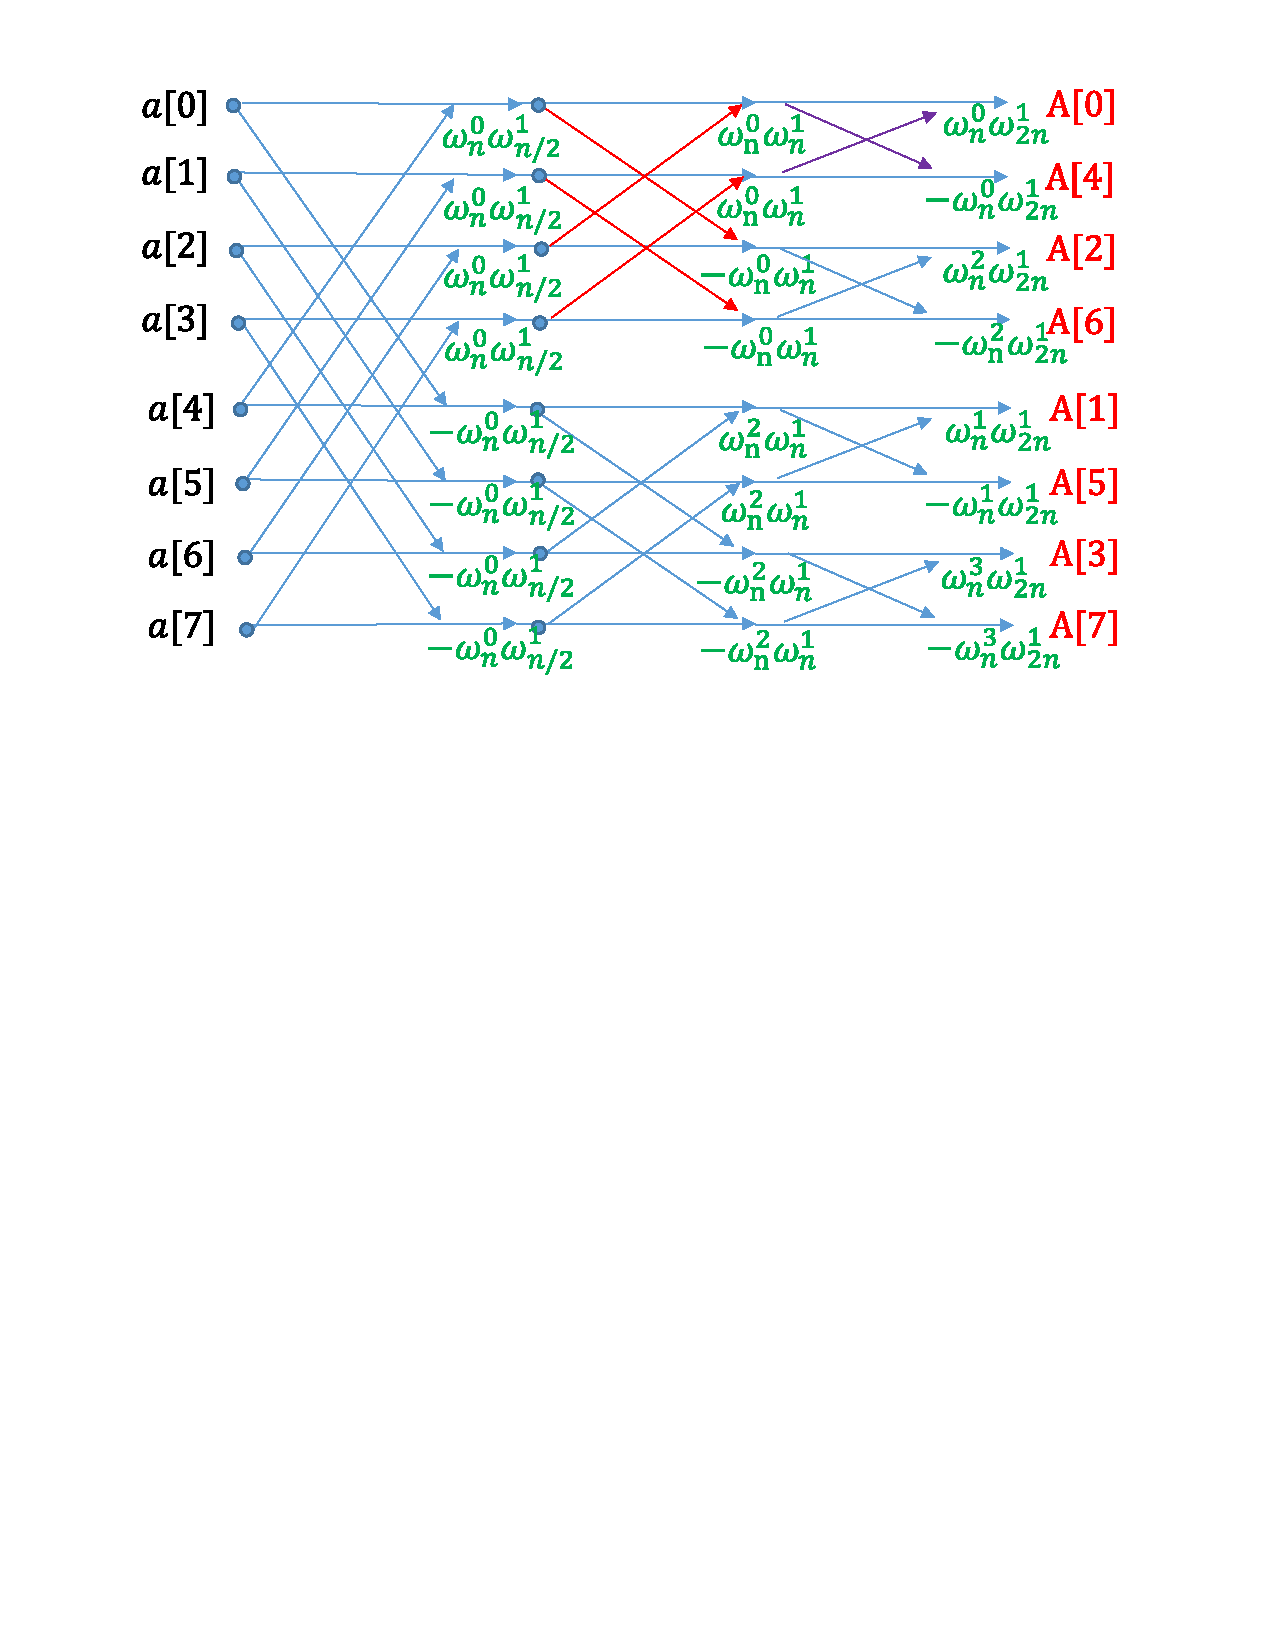
\includegraphics[width=\textwidth]{./fig/DIT1.pdf}
\caption{Generic architecture for NTT with merged twiddle factors ($N=8$)}
\label{fig:dit1}
\end{subfigure}

% \begin{subfigure}[t]{0.8\textwidth}\centering
% 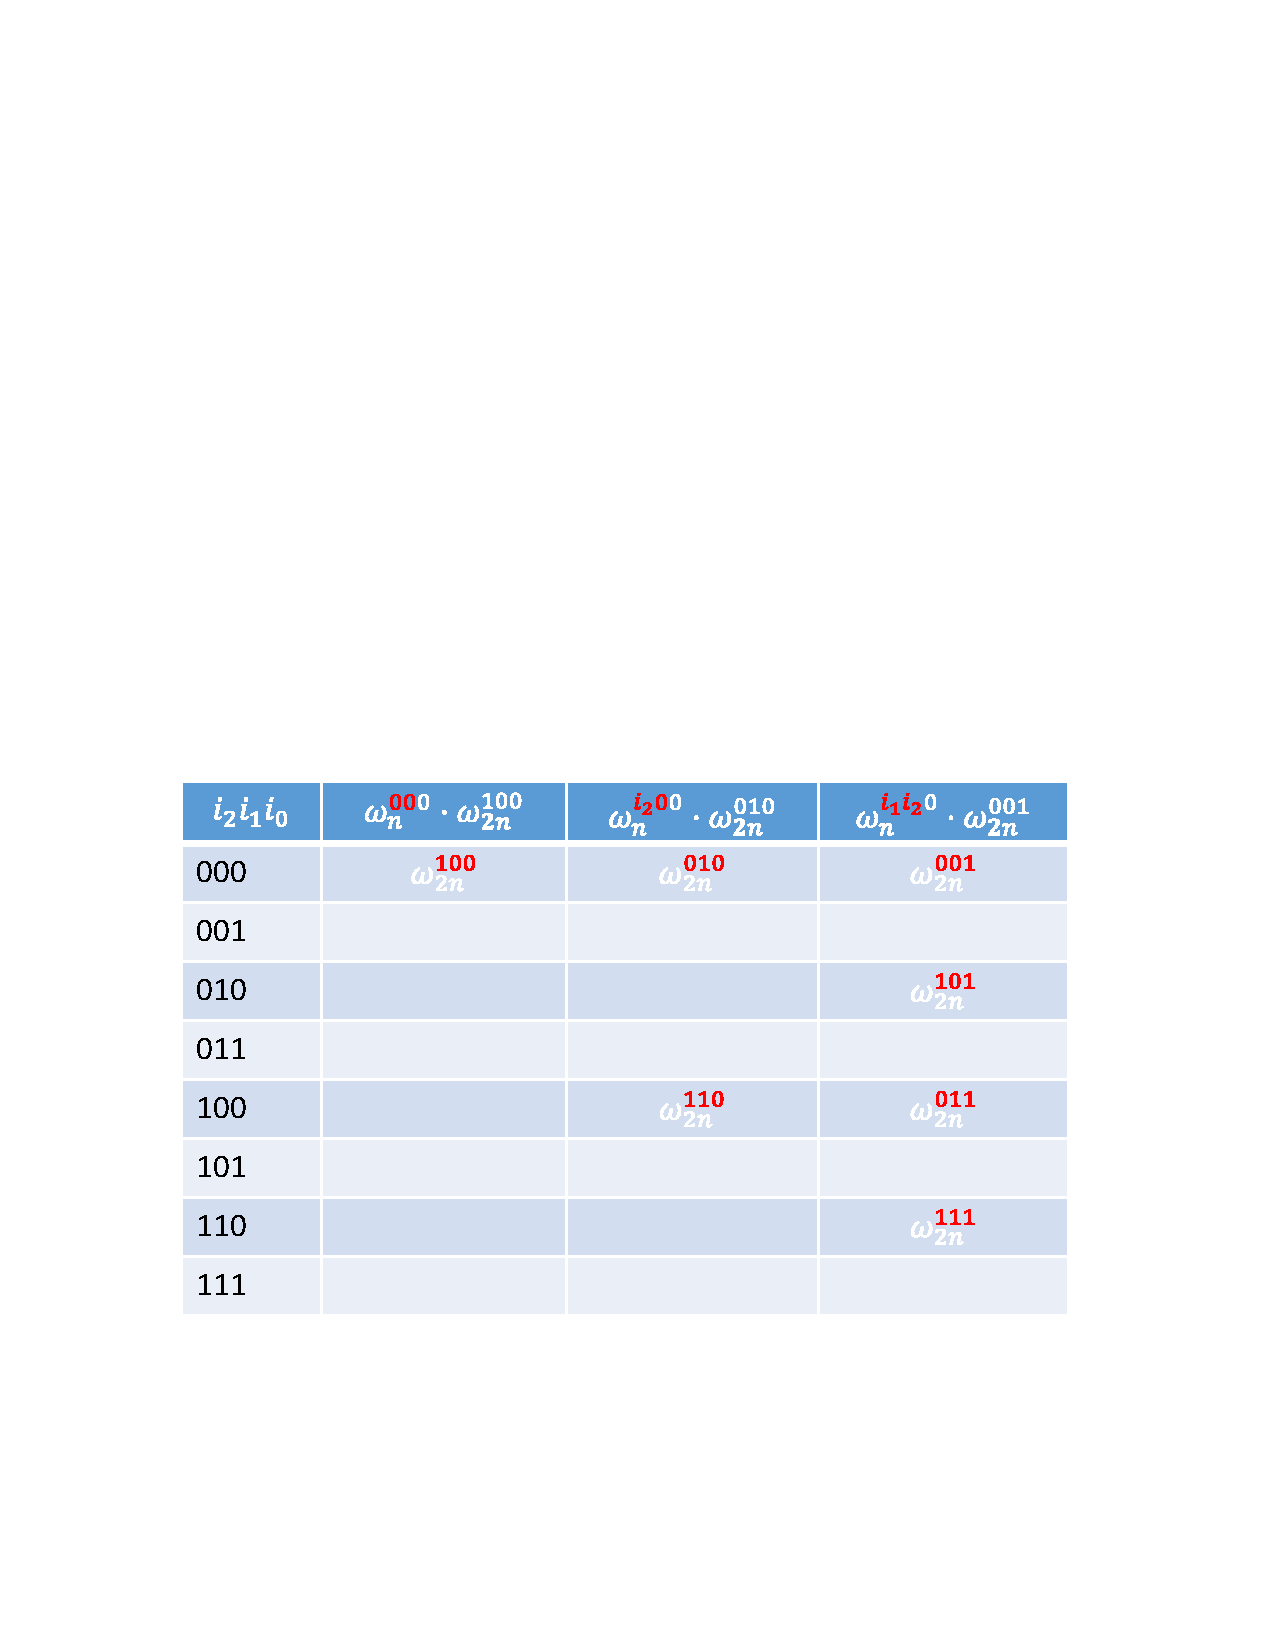
\includegraphics[width=\textwidth]{./fig/DIT2.pdf}
% \caption{Twiddle factor LUT context ($N=8$)}
% \label{fig:dit2}
% \end{subfigure}

\begin{subtable}[b]{0.8\textwidth}
  \centering
    \begin{tabular}{lccc}
     \hline
     $i=|i_2i_1i_0|_2$ & $\omega_N^{\textcolor{red}{00}}\cdot \omega_{2N}^{100}$ & $\omega_N^{\textcolor{red}{i_20}}\cdot \omega_{2N}^{010}$ & $\omega_N^{\textcolor{red}{i_1i_2}}\cdot \omega_{2N}^{001}$ \\
     \hline
     000 & \multirow{8}{*}{$\omega_{2N}^{\textcolor{red}{100}}$} & $\omega_{2N}^{\textcolor{red}{010}}$ & $\omega_{2N}^{\textcolor{red}{001}}$\\
     001 &                                      &                     &                     \\
     010 &                                      &                     & $\omega_{2N}^{\textcolor{red}{101}}$\\
     011 &                                      &                     &                     \\
     100 &                                      & $\omega_{2N}^{\textcolor{red}{110}}$ & $\omega_{2N}^{\textcolor{red}{011}}$\\
     101 &                                      &                     &                     \\
     110 &                                      &                     & $\omega_{2N}^{\textcolor{red}{111}}$\\
     111 &                                      &                     &                    \\
     \hline
     \end{tabular}
  \caption{Twiddle factor LUT context ($N=8$)}
  \label{table:table}
  \end{subtable}

\caption{DIT instance with $N=8$}
\end{figure*}


 % \begin{subtable}[!t]\centering
 % \caption{Twiddle factor LUT context ($N=8$)}
 % \label{table:gf2m-rollo-i}
 % \scalebox{1}{\begin{tabular}{lccc}
 % \hline
 % $i=|i_2i_1i_0|_2$ & $\omega_n^{\textcolor{red}{00}0}\cdot \omega_{2n}^{100}$ & $\omega_n^{\textcolor{red}{i_20}0}\cdot \omega_{2n}^{010}$ & $\omega_n^{\textcolor{red}{i_1i_2}0}\cdot \omega_{2n}^{001}$ \\
 % \hline
 % 000 & \multirow{8}{*}{$\omega_{2n}^{\textcolor{red}{100}}$} & $\omega_{2n}^{\textcolor{red}{010}}$ & $\omega_{2n}^{\textcolor{red}{001}}$\\
 % 001 &                                      &                     &                     \\
 % 010 &                                      &                     & $\omega_{2n}^{\textcolor{red}{101}}$\\
 % 011 &                                      &                     &                     \\
 % 100 &                                      & $\omega_{2n}^{\textcolor{red}{110}}$ & $\omega_{2n}^{\textcolor{red}{011}}$\\
 % 101 &                                      &                     &                     \\
 % 110 &                                      &                     & $\omega_{2n}^{\textcolor{red}{111}}$\\
 % 111 &                                      &                     &                    \\
 % \hline
 % \end{tabular}}
 % \end{subtable}


\subsection{$log_2d$-Dimensional Hypercube Multiprocessors}
\begin{figure*}[!tb]
\centering
\begin{subfigure}[t]{0.5\textwidth}\centering
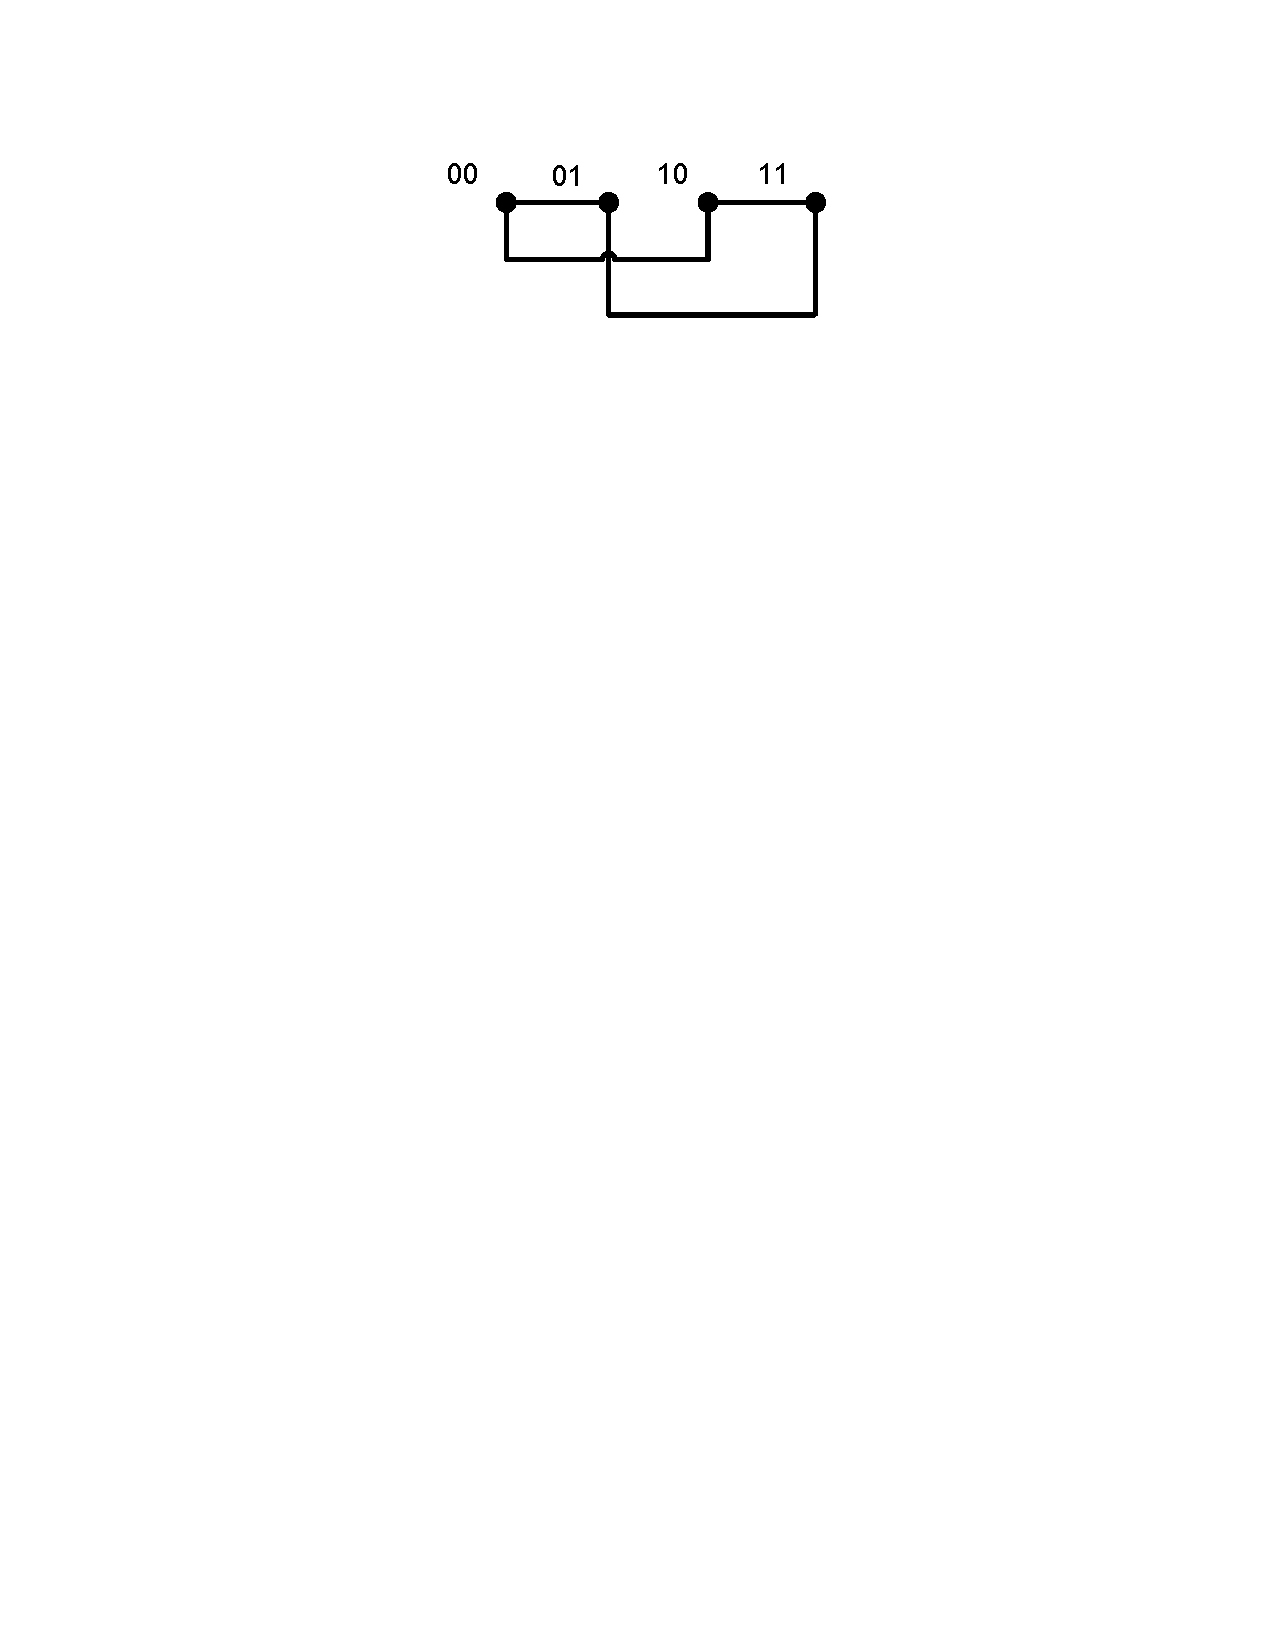
\includegraphics[width=\textwidth]{./fig/HyperCube1.pdf}
\caption{$d=4$, $ID\in\{P_0,P_1,P_2,P_3\}$}
\label{fig:hypercube4}
\end{subfigure}

\begin{subfigure}[t]{0.5\textwidth}\centering
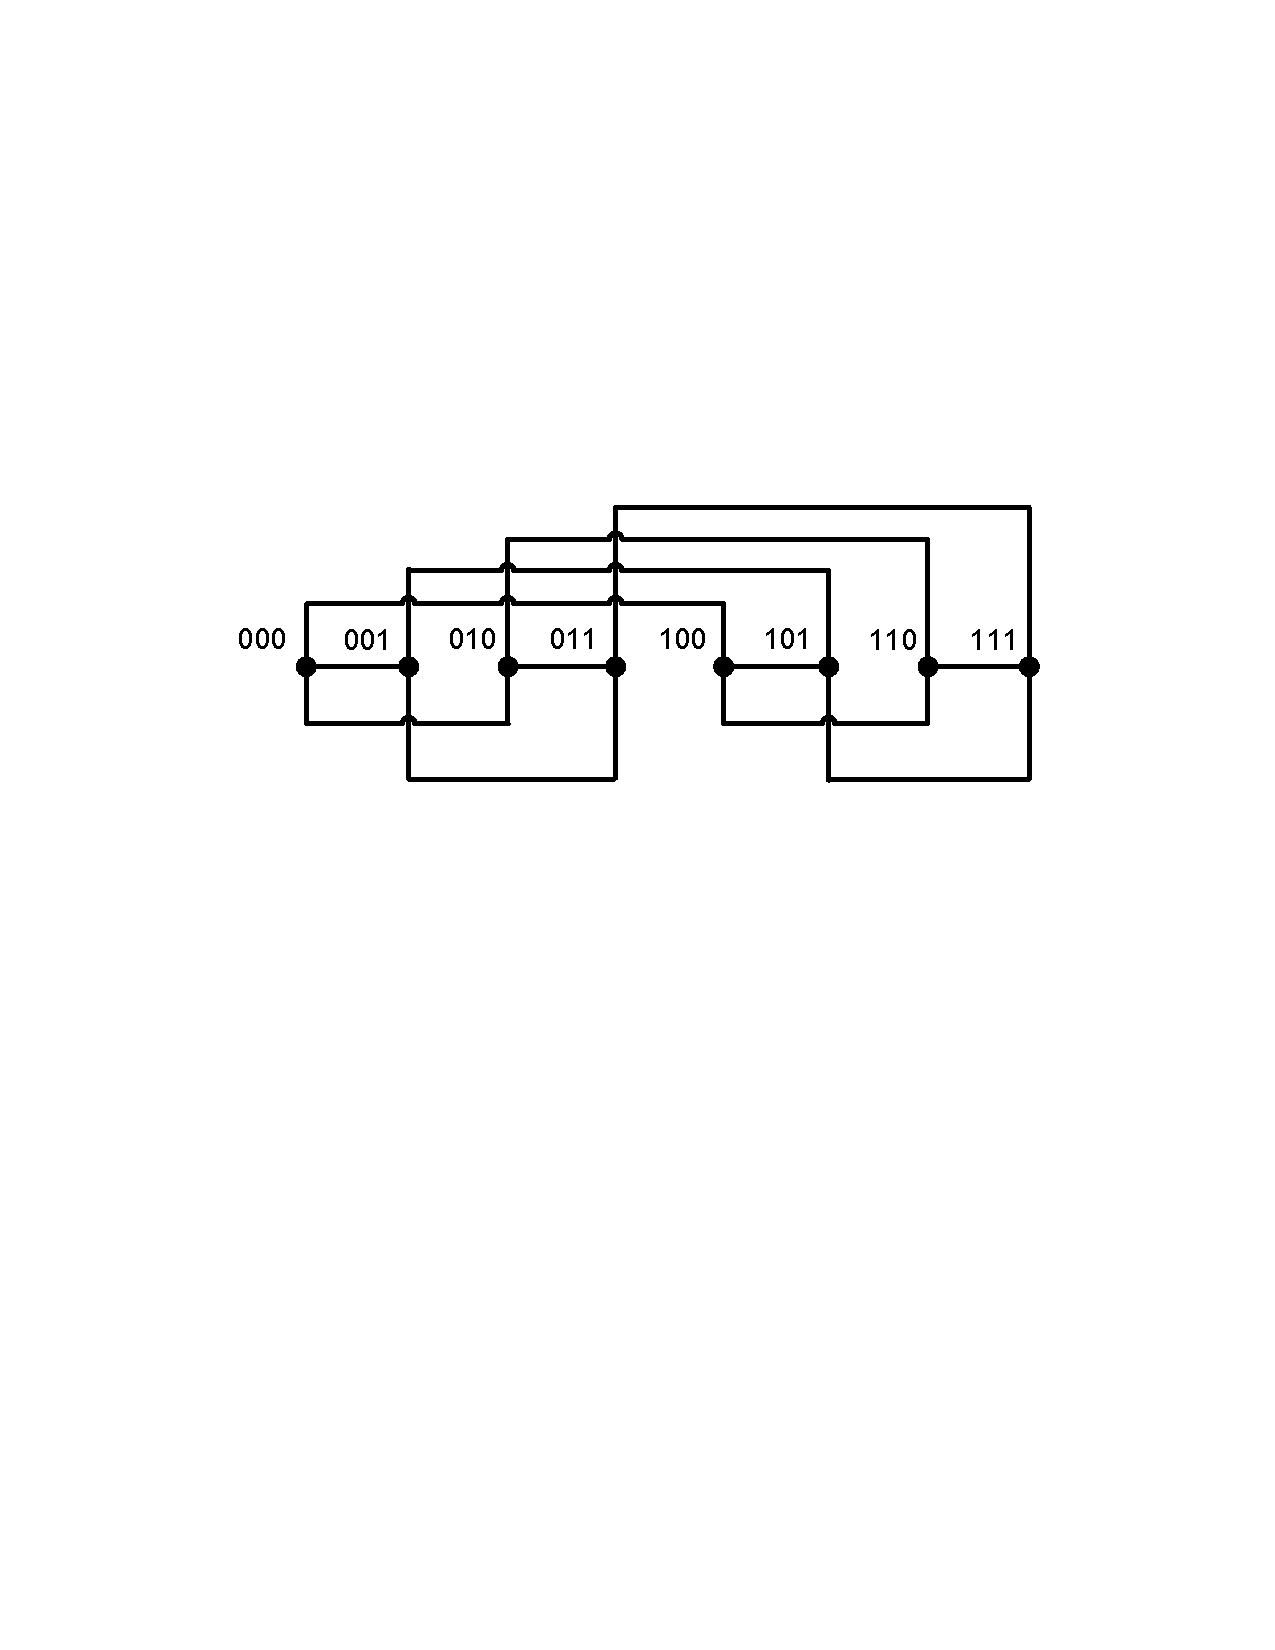
\includegraphics[width=\textwidth]{./fig/HyperCube2.pdf}
\caption{$d=8$, $ID\in\{P_0,P_1,P_2,P_3,P_4,P_5,P_6,P_7\}$}
\label{fig:hypercube8}
\end{subfigure}
\caption{Hypercubes of Dimension $log_2d=2$ and $log_2d=3$}
\end{figure*}

\begin{algorithm}[!tbh]
 \DontPrintSemicolon % Some LaTeX compilers require you to use \dontprintsemicolon instead
 \KwIn{$d$ node processors}
 \KwOut{$d$ node processors with connections}
    Denote the processor IDs as $\{P_0,P_1,\cdots,P_{d-1}\}$ where $d$ is a power-of-2\;
    \For{$i\leftarrow 0$ \KwTo $d-1$}{  
        $[i_{log_2d-1,\cdots,i_0}]_2 \gets BinRepr(i)$\;     
        \For{$j\leftarrow 0$ \KwTo $log_2d-1$}{
            flip the bit $i_j$ in $[i_{log_2d-1},\cdots,i_j,\cdots, i_0]_2$ to make $[i_{log_2d-1},\cdots,\bar{i_j},\cdots, i_0]_2$\;
            \uIf{$[i_{log_2d-1},\cdots,\bar{i_j},\cdots,i_0]_2 > [i_{log_2d-1},\cdots,i_j,\cdots,i_0]_2$}{
                  connect $P_{[i_{log_2d-1},\cdots,i_j,\cdots,i_0]_2}$ and $P_{[i_{log_2d-1},\cdots,\bar{i_j},\cdots,i_0]_2}$\;
                 }     
        }   
    }
    \Return {$(P_0,\cdots,P_{d-1})$\;}
 \caption{Construction of the $log_2d$-dimensional hypercube}\label{alg:descript_hypercube}
\end{algorithm}

\begin{algorithm}[!tbh]
 \DontPrintSemicolon % Some LaTeX compilers require you to use \dontprintsemicolon instead
 \KwIn{$log_2d$-dimensional hypercubes}
 \KwOut{communication pattern}
    Denote the processor IDs as $\{P_0,P_1,\cdots,P_{d-1}\}$\;
    \For{$k\leftarrow 0$ \KwTo $log_2d-1$}{  
        /*$d/2$ pairs of processors exchange data in step-$k$*/\;
        exchange data between processors $P_{[i_{log2d-1},\cdots,i_{log_2d-1-k},\cdots,0]_2}$ and $P_{[i_{log2d-1},\cdots,\overline{i_{log_2d-1-k}},\cdots,0]_2}$ which differ at $i_{log_2d-1-k}$\;        
    }   
    \Return {$c(x)$\;}
 \caption{Subcube-doubling communication in $log_2d$-dimensional hypercube}\label{alg:descript_subcube}
\end{algorithm}

\begin{table}[h!]\begin{center}
 \caption{Subcube-doubling communication in $3$-dimensional hypercube}\label{tab:descript_subcube}
\begin{tabular}{l c}
\hline
  steps & connections\\
\hline
  Step-(0) & \raisebox{-0.5\height}{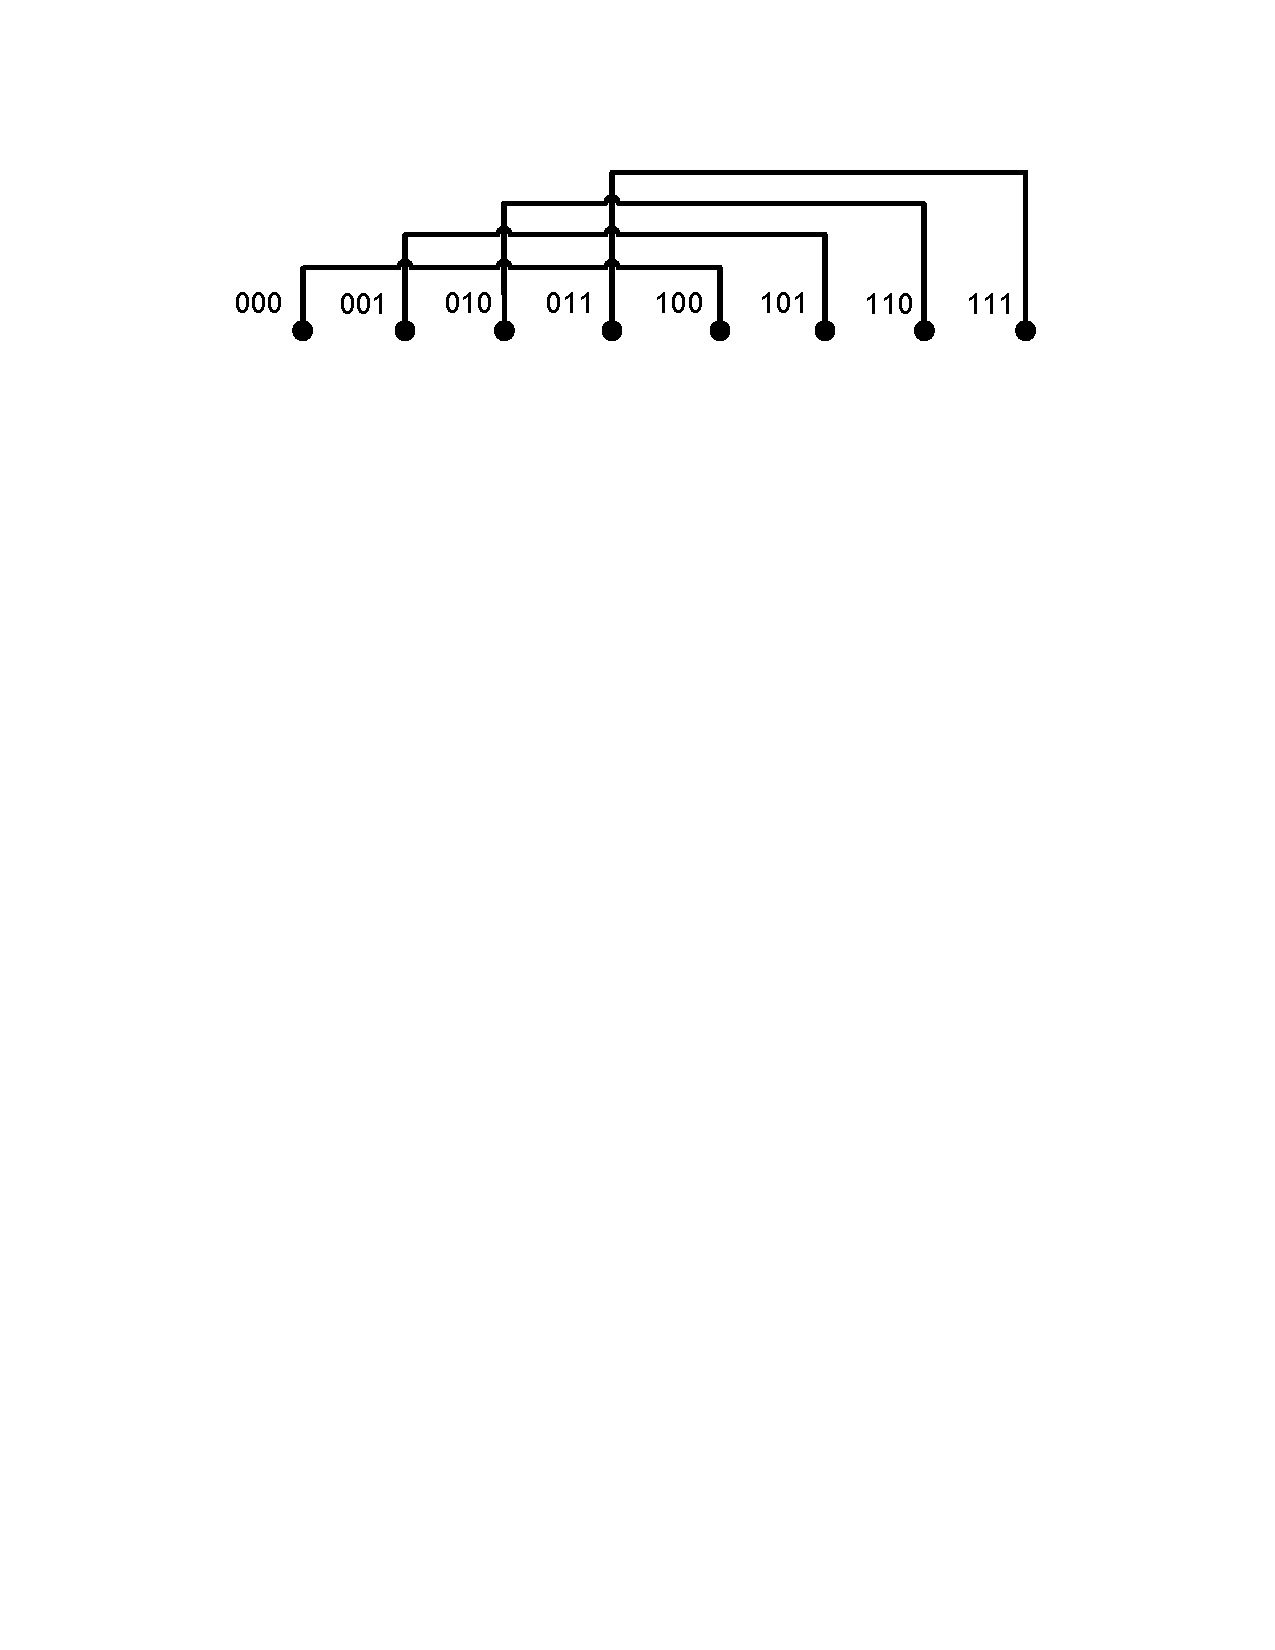
\includegraphics[width=.6\textwidth]{./fig/subcube_comm1.pdf}}\\
  Step-(1) & \raisebox{-0.5\height}{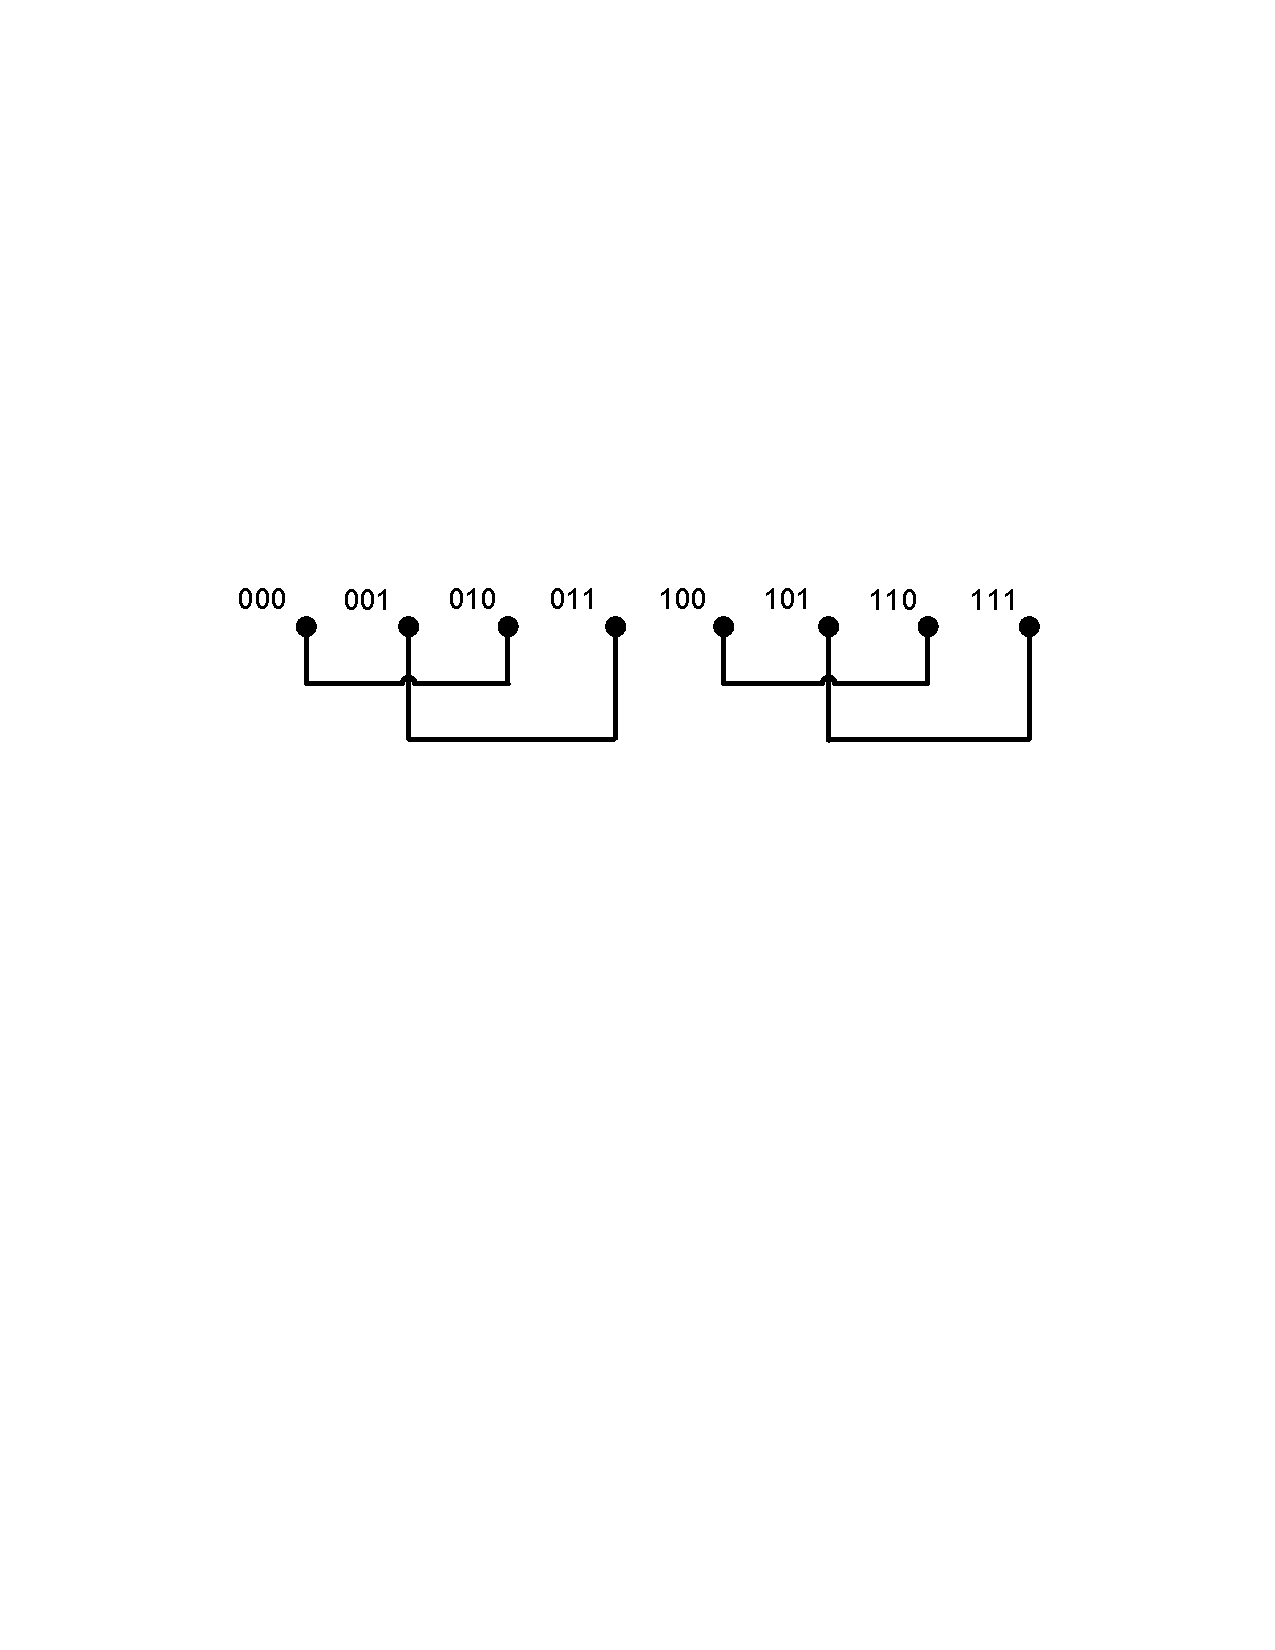
\includegraphics[width=.6\textwidth]{./fig/subcube_comm2.pdf}}\\
  Step-(2) & \raisebox{-0.5\height}{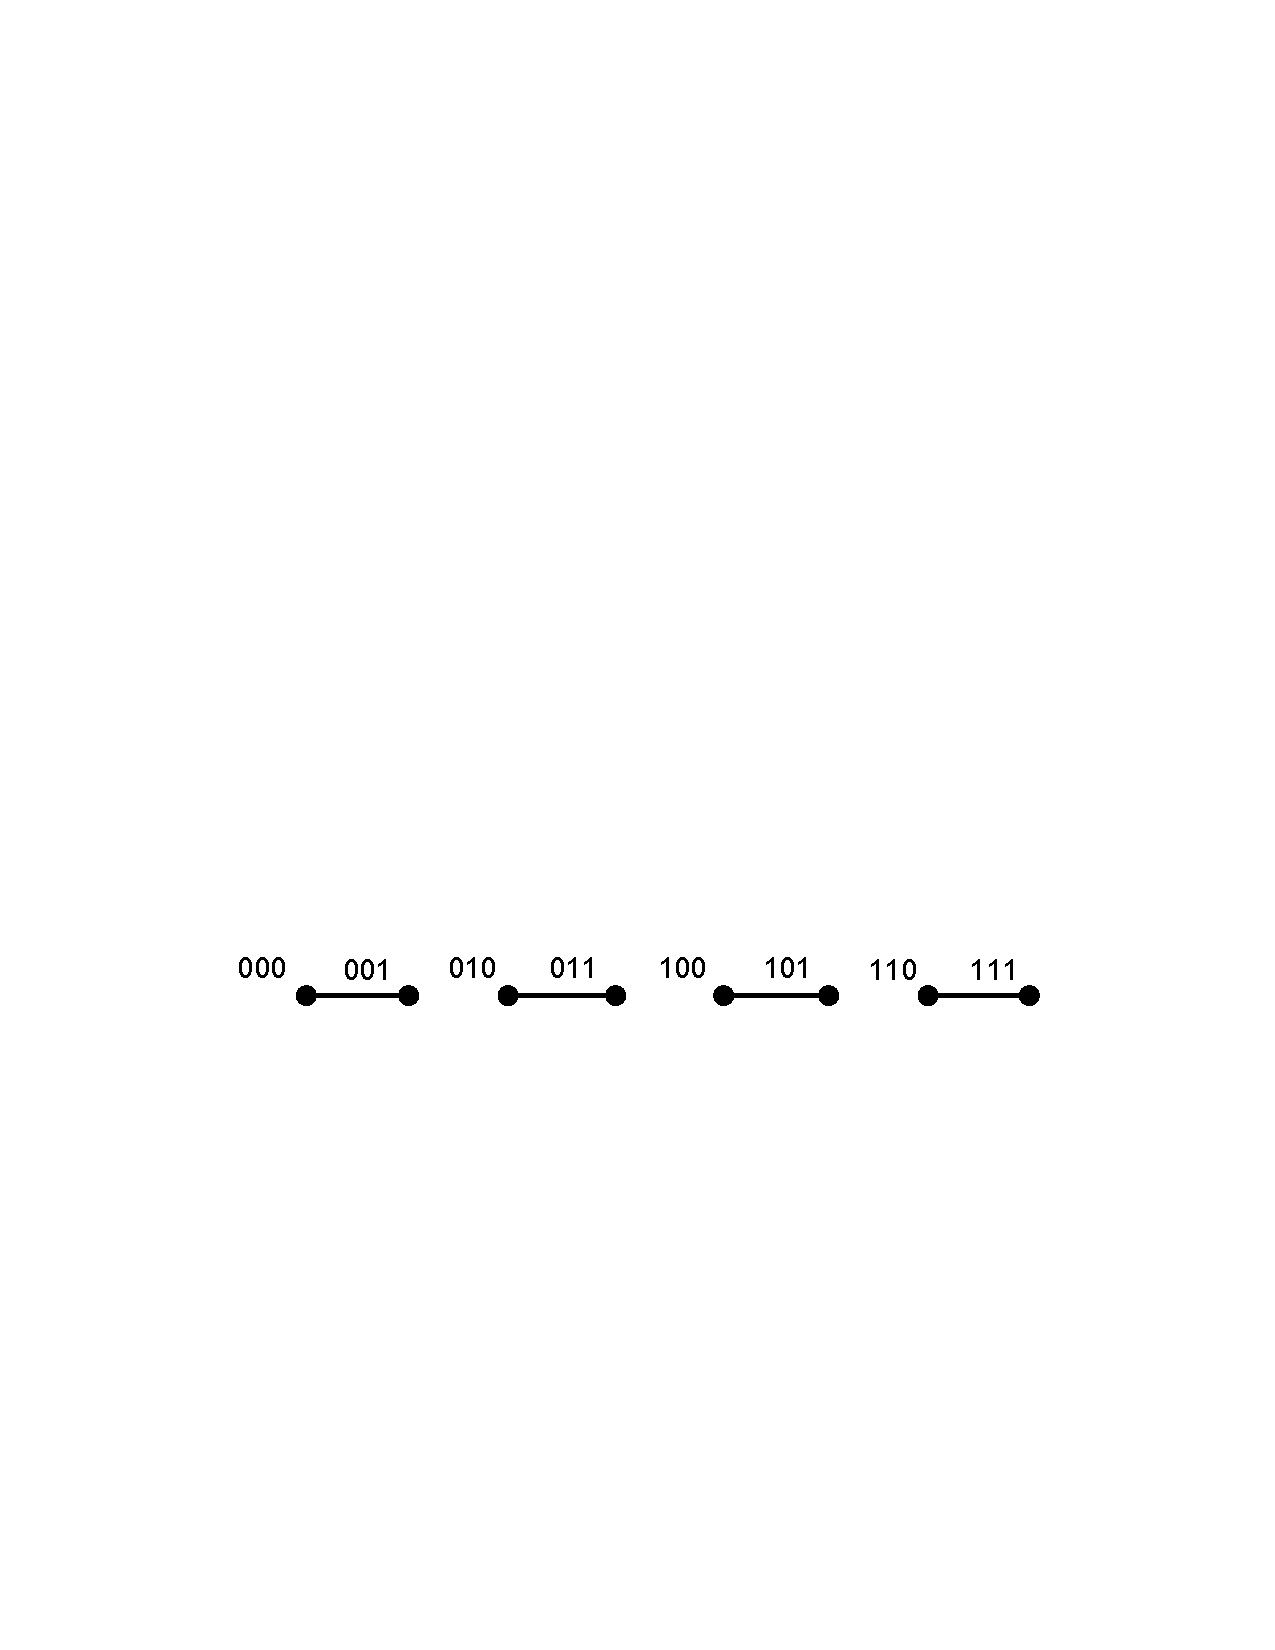
\includegraphics[width=.6\textwidth]{./fig/subcube_comm3.pdf}}\\
\hline  
\end{tabular}\end{center}  
\end{table}

In this subsection, we introduce the hypercube topology which fits the parallelized version of NTT algorithm. The hypercube is also the basis for hardware architecture proposed in this work.

Before detailing the parallel NTT algorithm and hardware, the computing model used in this paper must be clarified. There are $d$ identical node processors organized in a hypercube of dimension $log_2d$. Each node processor includes one butterfly unit and some storage ($N/d$ NTT points). Roughly speaking, this $log_2d$-dimensional hypercube structure should increase the speed of sequential NTT algorithm by $d$ times. Fig.~\ref{fig:hypercube4} illustrates the hypercube architecture of dimension $2$ where $4$ node processors (\textit{i.e.}, $P_0,P_1,P_2,P_3$ labeled as it binary form '00', '01', '10', and '11') are implemented. The node processors are sparsely connected with each other where any one of them are connected to the other 2 processors. For example, $P_0$ is only connected to $P_1$ and $P_2$,  $P_1$ is only connected to $P_0$ and $P_3$.
Fig.~\ref{fig:hypercube8} illustrates the hypercube architecture of dimension $3$ where $8$ node processors (\textit{i.e.}, $P_0,P_1,\cdots,P_7$ labeled as it binary form '000', '001', ..., and '111') are implemented. The node processors are sparsely connected with each other where any one of them are connected to the other 3 processors. For example, $P_0$ is only connected to $P_1$, $P2$ and $P4$,  $P_1$ is only connected to $P_0$, $P_3$ and $P_5$.


Alg.~\ref{alg:descript_hypercube} formally describes how to construct the $log_2d$-dimensional hypercube by sparsely connecting $d$ node processors. The key idea here is that for each processor $P_i$, rewrite the index $i$ in binary form as $[i_{log_2d-1},\cdots,i_0]_2$, and connects those processors $P_j$ whose index $j=[j_{log_2d-1},\cdots,j_0]_2$ differs only 1 bit compared with $i$. In particular, each node processor connects only to $log_2d$ other node processors in this $log_2d$-dimensional hypercube topology. The if condition in the for-loop in Alg.~\ref{alg:descript_hypercube} helps rule out the possibility of connecting the same pair of nodes repeatedly.
{}
When the computation continues in the hypercube, the intermediate data generated in each round of computations typically requires exchange between node processors. This type of data exchange is referred to as `subcube-doubling' communication in the literature. There are in total $log_2d$ rounds of exchange during the communication as described in Alg.~\ref{alg:descript_subcube}: In step-($k$), each node processor $P_i$ with index $i=[i_{log_2d-1},\cdots,i_{0}]_2$ exchanges data with $P_j$ whose index $j$ differs at the $log_2d-1-k$-th bit. 

An illustration instance with $d=8$ for subcube-doubling algorithm (Alg.~\ref{alg:descript_subcube}) is given in Table~\ref{tab:descript_subcube}. $log_2d=3$ communication steps are required in this example: In step-(0), processor $P_{[i_{2},i_{1},i_{0}]_2}$ connects processor $P_{[\overline{i_{2}},i_{1},i_{0}]_2}$ which differs at $i_{2}$, and there are $d/2=4$ such pairs of connections, \textit{i.e.}, $P_0-P_4, P_1-P_5, P_2-P_6, P_3-P_7$; In step-(1), processor $P_{[i_{2},i_{1},i_{0}]_2}$ connects processor $P_{[i_{2},\overline{i_{1}},i_{0}]_2}$ which differs at $i_{1}$; Finally, in step-(2), processor $P_{[i_{2},i_{1},i_{0}]_2}$ connects processor $P_{[i_{2},i_{1},\overline{i_{0}}]_2}$ which differs at $i_{0}$.


\subsection{A Useful Equivalent Notation: |PID|Local $M$}
Assume that $N$ points are stored in the global array $a[\cdot]=\{a_{N-1},\cdots,0\}$ or simplified as $a[\cdot]=\{a_i\}_{i=N-1,\cdots,0}$, and the elements in the array are assigned evenly to $d$ node processors for storage and processing. Then the array address based notation uses a $log N$-bit integer $i={i_{logN-1}\cdots i_0}_2$:
\[
  i_{logN-1}\cdots i_{k+1}|i_k\cdots i_{k-logd+1}|i_{k-logd}\cdots i_0
\]
to indicate that cosecutive $logd$ bits $i_k\cdots i_{k-logd+1}$ are chosen to specify the data-to-processor allocation.

In general, since any $logd$ bits can be used to form the processor ID number, it is easier to concatenate the bits representing the processor ID into one group denoted by `PID', and refers to the remaining $logN-logd$ bits, which are concatenated to form the local array address, as `Local $M$'. This paper uses the following equivalent notation, where the leading $d$ bits are always used to identify the processor ID number.
\[
  |\text{PID}|\text{Local } M = |\underbrace{i_k\cdots i_{k-logd+1}}_{logd}|\overbrace{i_{N-1}\cdots i_{k+2}i_{k+1}}^{N-k-1}\overbrace{i_{k-d}\cdots i_1i_0}^{k-logd+1}
\]


Table~\ref{tab:pid_notation2} shows the details about the data allocation for hypercube processor array after a naturally ordered input series of $N=32$ elements are divided among $d=4$ processors using one particular cyclic block mapping $i_4i_3$|$i_2i_1i_0$. For instance, to locate $a_m=a_{26}$, one writes down $m=26=11010_2=i_4i_3i_2i_1i_0$, from which one knows that $a_{26}$ is stored in $a[r]$, $r=i_4i_3|i_2i_1i_0=11|010_2=26$, meaning that $a[26]=a_{26}$ (the element $a_{26}$ is located in $a[26]$) is allocated by processor $P_{i_4i_3}=P_{01}$.

\begin{table}[h!]\begin{center}
 \caption{Local data in processor $P_{i_4i_3}$ expressed in terms of global array element $a[m],m=i_4i_3i_2i_1i_0$ for the notation $i_4i_3$|$i_2i_1i_0$}\label{tab:pid_notation2}
\scalebox{0.8}{\begin{tabular}{c c | c c | c c | c c}
\hline
  \tabincell{c}{|PID|Local $M$\\$i_4i_3$|$i_2i_1i_0$} & \tabincell{c}{$P_{i_4i_3}=P_{00}$\\$a[m]$} & \tabincell{c}{|PID|Local $M$\\$i_4i_3$|$i_2i_1i_0$} & \tabincell{c}{$P_{i_4i_3}=P_{01}$\\$a[m]$} &\tabincell{c}{|PID|Local $M$\\$i_4i_3$|$i_2i_1i_0$} & \tabincell{c}{$P_{i_4i_3}=P_{10}$\\$a[m]$} & \tabincell{c}{|PID|Local $M$\\$i_4i_3$|$i_2i_1i_0$} & \tabincell{c}{$P_{i_4i_3}=P_{11}$\\$a[m]$}\\
\hline
$00$|$000$ & $a[0]$ & $01$|$000$ & $a[8]$ & $10$|$000$ & $a[16]$ & $11$|$000$ & $a[24]$\\
$00$|$001$ & $a[1]$ & $01$|$000$ & $a[9]$ & $10$|$000$ & $a[17]$ & $11$|$000$ & $a[25]$\\
$00$|$010$ & $a[2]$ & $01$|$000$ & $a[10]$ & $10$|$000$ & $a[18]$ & $11$|$000$ & $a[26]$\\
$00$|$011$ & $a[3]$ & $01$|$000$ & $a[11]$ & $10$|$000$ & $a[19]$ & $11$|$000$ & $a[27]$\\
$00$|$100$ & $a[4]$ & $01$|$000$ & $a[12]$ & $10$|$000$ & $a[20]$ & $11$|$000$ & $a[28]$\\
$00$|$101$ & $a[5]$ & $01$|$000$ & $a[13]$ & $10$|$000$ & $a[21]$ & $11$|$000$ & $a[29]$\\
$00$|$110$ & $a[6]$ & $01$|$000$ & $a[14]$ & $10$|$000$ & $a[22]$ & $11$|$000$ & $a[30]$\\
$00$|$111$ & $a[7]$ & $01$|$000$ & $a[15]$ & $10$|$000$ & $a[23]$ & $11$|$000$ & $a[31]$\\
\hline  
\end{tabular}}
\end{center}\end{table}

On the other hand, when the input elements are stored in $\mathbf{a}$ in bit-reversed order, \textit{i.e.,} $a[r]=a_m$ where $m=i_{n-1}i_{n-2}\cdots i_{0}$, and $r=i_0\cdots i_{n-2}i_{n-1}$, then the equivalent notation is as follows:
\[
  |\text{PID}|\text{Local } M = |\underbrace{i_{k-logd+1}\cdots i_{k}}_{logd}|\overbrace{i_{0}\cdots i_{k-logd}}^{k-logd+1}\overbrace{i_{k+1}\cdots i_{n-1}}^{N-k-1}
\]

\begin{table}[h!]\begin{center}
 \caption{Local data in processor $P_{i_0i_1}$ (bit reversed) expressed in terms of global array element $a[r]=a_m,r=i_0i_1i_2i_3i_4,m=i_4i_3i_2i_1i_0$ for the notation $i_0i_1$|$i_2i_3i_4$}\label{tab:pid_notation}
\scalebox{0.8}{\begin{tabular}{c c | c c | c c | c c}
\hline
  \tabincell{c}{|PID|Local $M$\\$i_0i_1$|$i_2i_3i_4$} & \tabincell{c}{$P_{i_0i_1}=P_{00}$\\$a[r]$} & \tabincell{c}{|PID|Local $M$\\$i_0i_1$|$i_2i_3i_4$} & \tabincell{c}{$P_{i_0i_1}=P_{01}$\\$a[r]$} &\tabincell{c}{|PID|Local $M$\\$i_0i_1$|$i_2i_3i_4$} & \tabincell{c}{$P_{i_0i_1}=P_{10}$\\$a[r]$} & \tabincell{c}{|PID|Local $M$\\$i_0i_1$|$i_2i_3i_4$} & \tabincell{c}{$P_{i_0i_1}=P_{11}$\\$a[r]$}\\
\hline
$00$|$000$ & $a[0]$ & $01$|$000$ & $a[8]$ & $10$|$000$ & $a[16]$ & $11$|$000$ & $a[24]$\\
$00$|$001$ & $a[1]$ & $01$|$000$ & $a[9]$ & $10$|$000$ & $a[17]$ & $11$|$000$ & $a[25]$\\
$00$|$010$ & $a[2]$ & $01$|$000$ & $a[10]$ & $10$|$000$ & $a[18]$ & $11$|$000$ & $a[26]$\\
$00$|$011$ & $a[3]$ & $01$|$000$ & $a[11]$ & $10$|$000$ & $a[19]$ & $11$|$000$ & $a[27]$\\
$00$|$100$ & $a[4]$ & $01$|$000$ & $a[12]$ & $10$|$000$ & $a[20]$ & $11$|$000$ & $a[28]$\\
$00$|$101$ & $a[5]$ & $01$|$000$ & $a[13]$ & $10$|$000$ & $a[21]$ & $11$|$000$ & $a[29]$\\
$00$|$110$ & $a[6]$ & $01$|$000$ & $a[14]$ & $10$|$000$ & $a[22]$ & $11$|$000$ & $a[30]$\\
$00$|$111$ & $a[7]$ & $01$|$000$ & $a[15]$ & $10$|$000$ & $a[23]$ & $11$|$000$ & $a[31]$\\
\hline  
\end{tabular}}
\end{center}\end{table}

Table~\ref{tab:pid_notation} shows the details about the data allocation for hypercube processor array after an inverse ordered input series of $N=32$ elements are divided among $d=4$ processors using one particular cyclic block mapping $i_0i_1$|$i_2i_3i_4$.
For instance, to locate $a_m=a_{26}$, one writes down $m=26=11010_2=i_4i_3i_2i_1i_0$, from which one knows that $a_{26}$ is stored in $a[r]$, $r=i_0i_1|i_2i_3i_4=01|011_2=11$, meaning that $a[11]=a_{26}$ (the element $a_{26}$ is located in $a[11]$) is allocated by processor $P_{i_0i_1}=P_{01}$.

\subsection{First attempt: parallel in-place FFTs without inter-processor permutations}

Consider the $DIT_{NN\to RN}$ algorithm (Alg.~\ref{alg:descript_ntt}) and use the cyclic block mapping introduced in the last subsection. For $N=32, d=4$, the computation is depicted below:

\begin{table}[h!]\begin{center}
\scalebox{0.8}{\begin{tabular}{c c c c c c}
\hline
$|i_4i_3|i_2i_1i_0$ & $|\overset{\blacktriangledown}{\underset{\triangle}{i_4}}i_3|i_2i_1i_0$ & $|\tau_4\overset{\blacktriangledown}{\underset{\triangle}{i_3}}|i_2i_1i_0$ & $|\tau_4\tau_3|\overset{\blacktriangledown}{i_2}i_1i_0$ & $|\tau_4\tau_3|\tau_2\overset{\blacktriangledown}{i_1}i_0$ & $|\tau_4\tau_3|\tau_2\tau_1\overset{\blacktriangledown}{i_0}$\\
Initial Map   &   $\Longleftarrow\Longrightarrow$ &  $\Longleftarrow\Longrightarrow$ \\
\hline
\end{tabular}}
\end{center}\end{table}

The initial map indicates that the processor $P_k$ initially holds the elements $a[8k],\cdots ,a[8k+7]$ for $k=0,1,2,3$.
The shorthand notation previously used for sequential NTT is augmented by two additional symbols. The double-headed arrow $\Longleftarrow\Longrightarrow$ indicates that $\frac{N}{d}$ data elements must be exchanged between processors in advance of butterfly computation. In our example, the NTT takes 5 rounds where the first two rounds require data exchange among proessors and the last three rounds do not require data exchange. The symbol $i_k$ identifies two things:
\begin{itemize}
  \item First, it indicates the input source of external data: the incoming data from another processor are the elements whose addresses differ from a processor's own data in bit $i_k$.
  \item Second, it indicates that all pairs of processors whose binary ID number differ in bit $i_k$ send each other a copy of their own data.
\end{itemize}

The required data communications before the first stage of butterfly computation (step-0) are explicitly depicted in Fig.~\ref{fig:dataswap_without_perm1} and Fig.~\ref{fig:dataswap_without_perm2}:  $P_0$ swaps data with $P_2$ such that $a[i]$ pairs with $a[i+16]$ to perform the required butterfly computation in the same processor for $i=0,\cdots,7$, and $P_1$ swaps data with $P_3$ such that $a[i]$ pairs with $a[i+16]$ to perform the required butterfly computation in the same processor for $i=8,\cdots,15$; the required data communications before the second stage of butterfly computation (step-1) are depicted in Fig.~\ref{fig:dataswap_without_perm3} and Fig.~\ref{fig:dataswap_without_perm4}: $P_0$ swaps data with $P_1$ such that $a[i]$ pairs with $a[i+8]$ to perform the required butterfly computation in the same processor for $i=0,\cdots,7$, and $P_2$ swaps data with $P_3$ such that $a[i]$ pairs with $a[i+8]$ to perform the required butterfly computation in the same processor for $i=16,\cdots,23$. The last three steps (step-2,3,4) do not require data swaps since all elements needed for butterfly computataion are already within the precessor: for example, in step-2, $a[0]$ pairs $a[4]$, $a[1]$ pairs $a[5]$, $a[2]$ pairs $a[6]$, $a[3]$ pairs $a[7]$, which are all located within processor $P_0$. 

\begin{figure*}[!tb]
\centering
\begin{subfigure}[b]{0.47\textwidth}
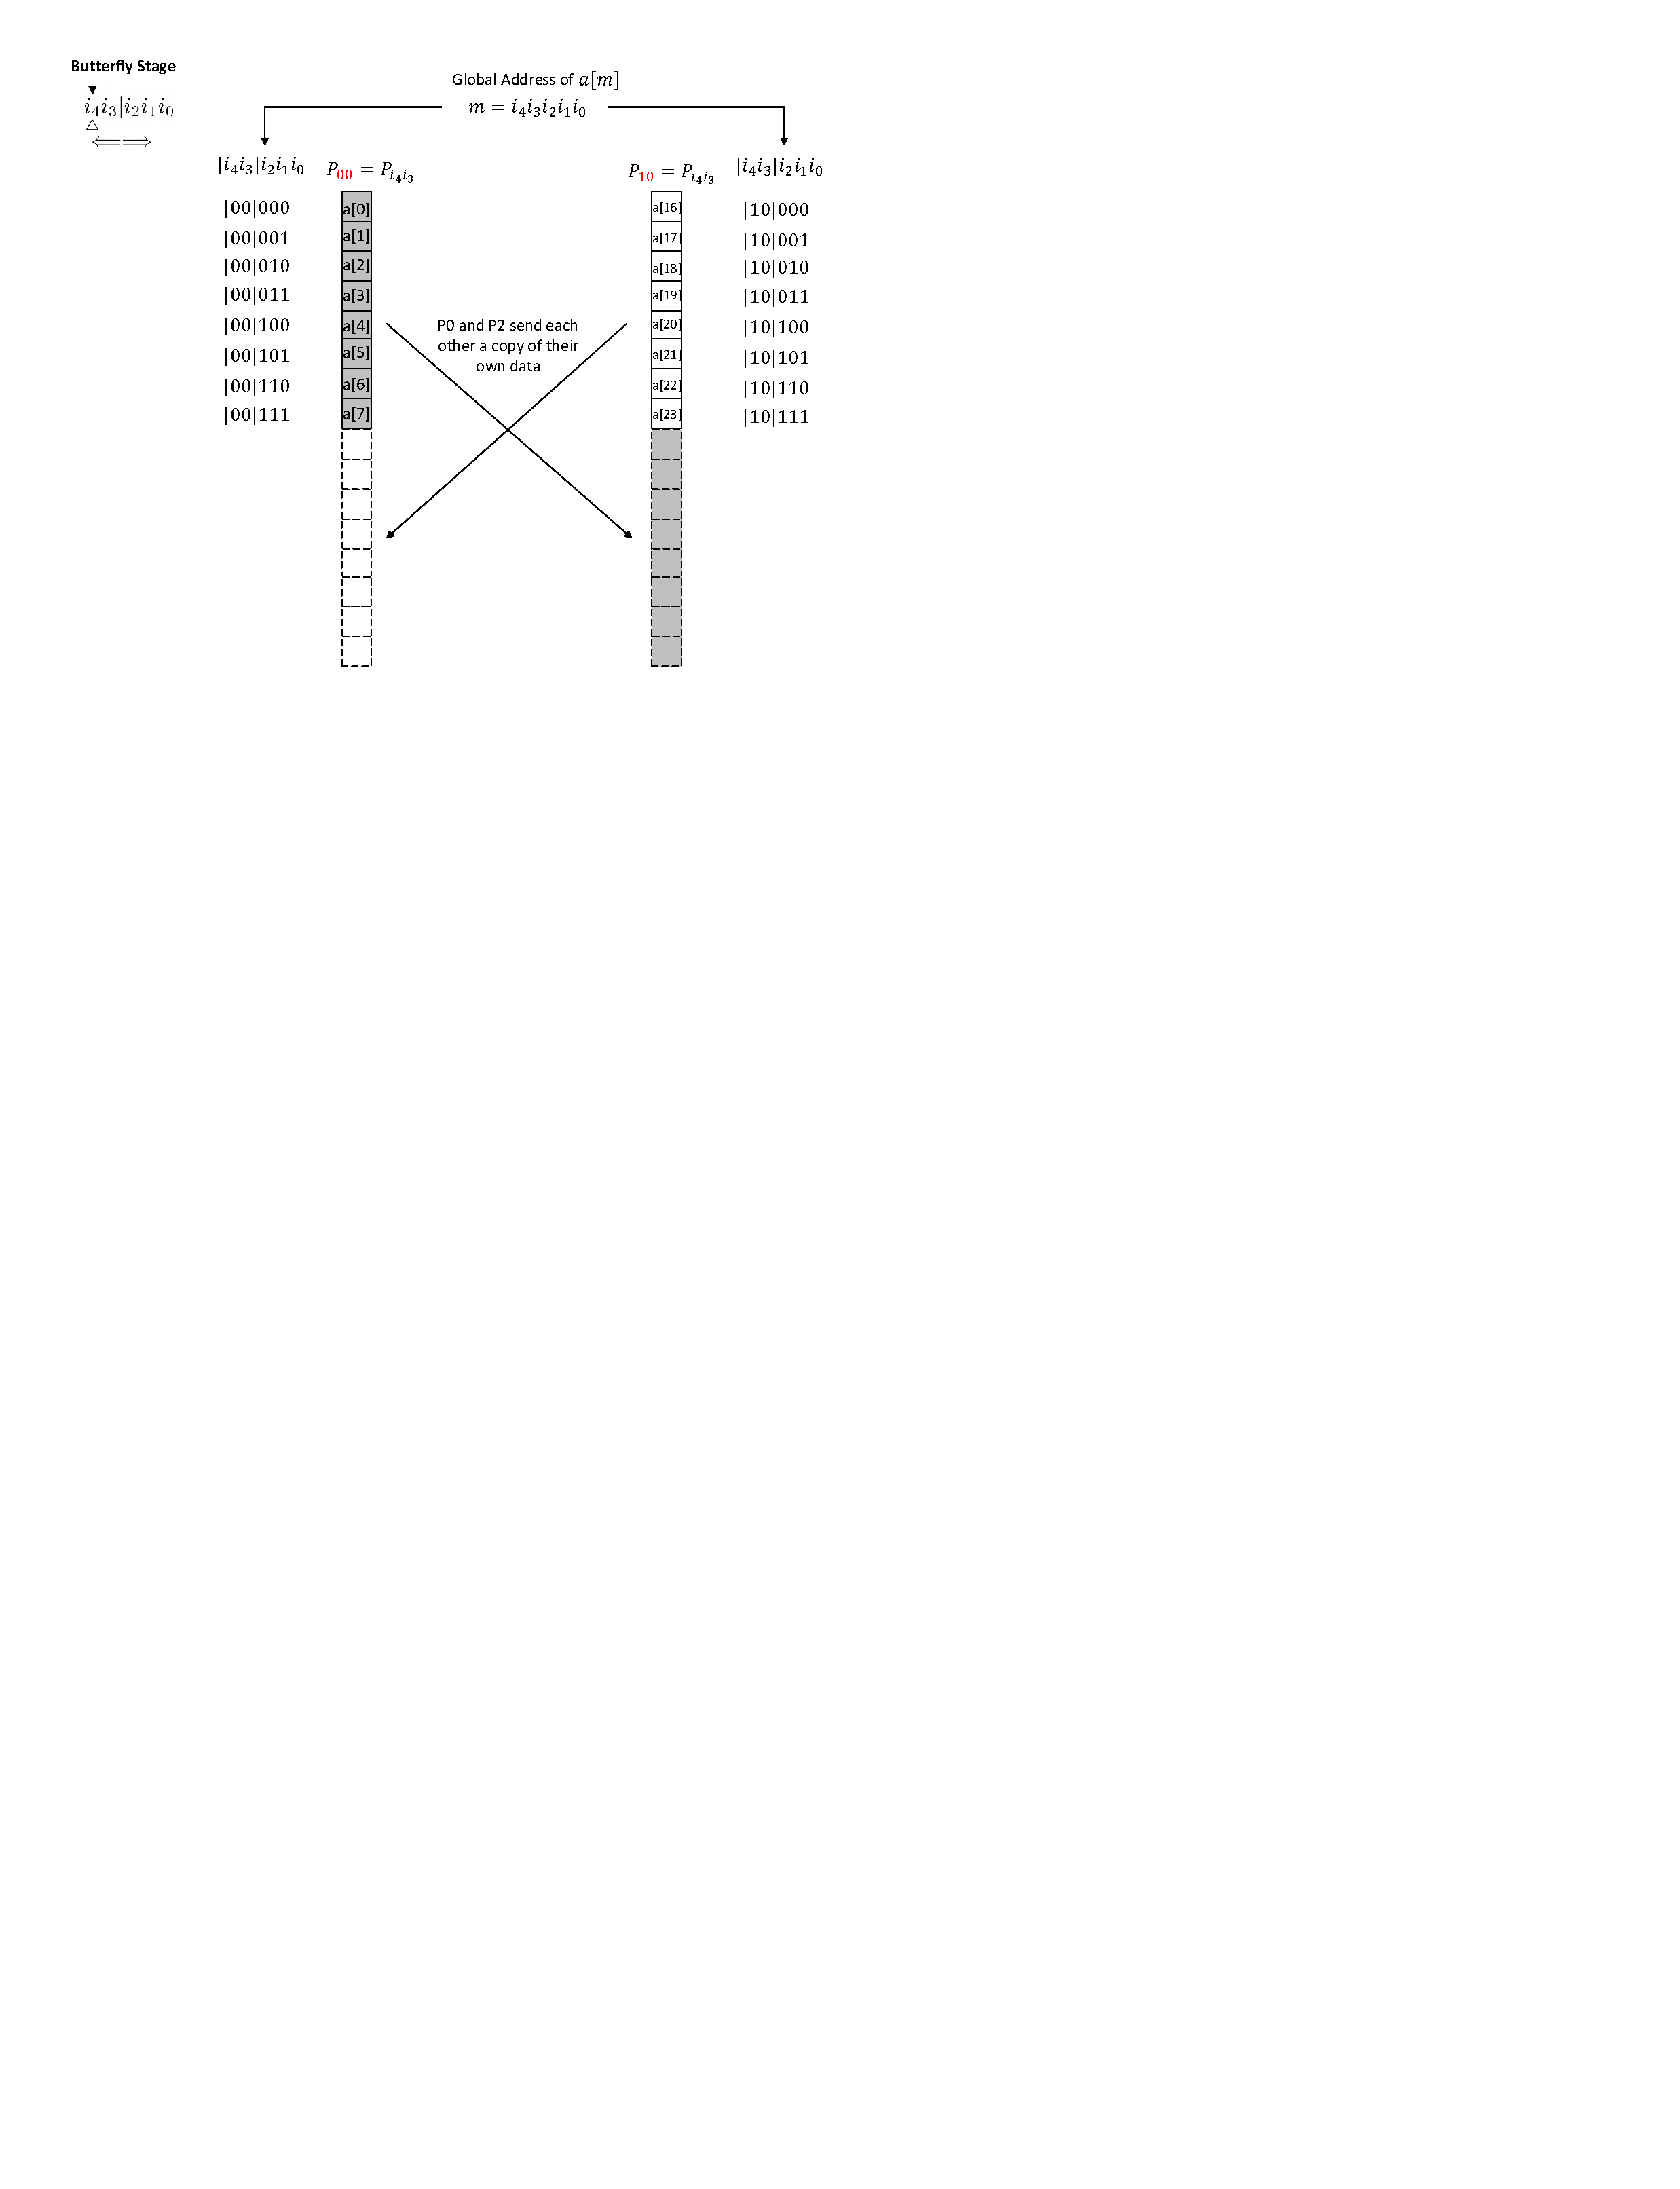
\includegraphics[width=\textwidth]{./fig/DataSwapWithoutPerm1.pdf}
\caption{In round-0, Data sent and received by processors $P_0$ and $P_2$}\label{fig:dataswap_without_perm1}
\end{subfigure}
\hspace{1em}
\begin{subfigure}[b]{.47\textwidth}\centering
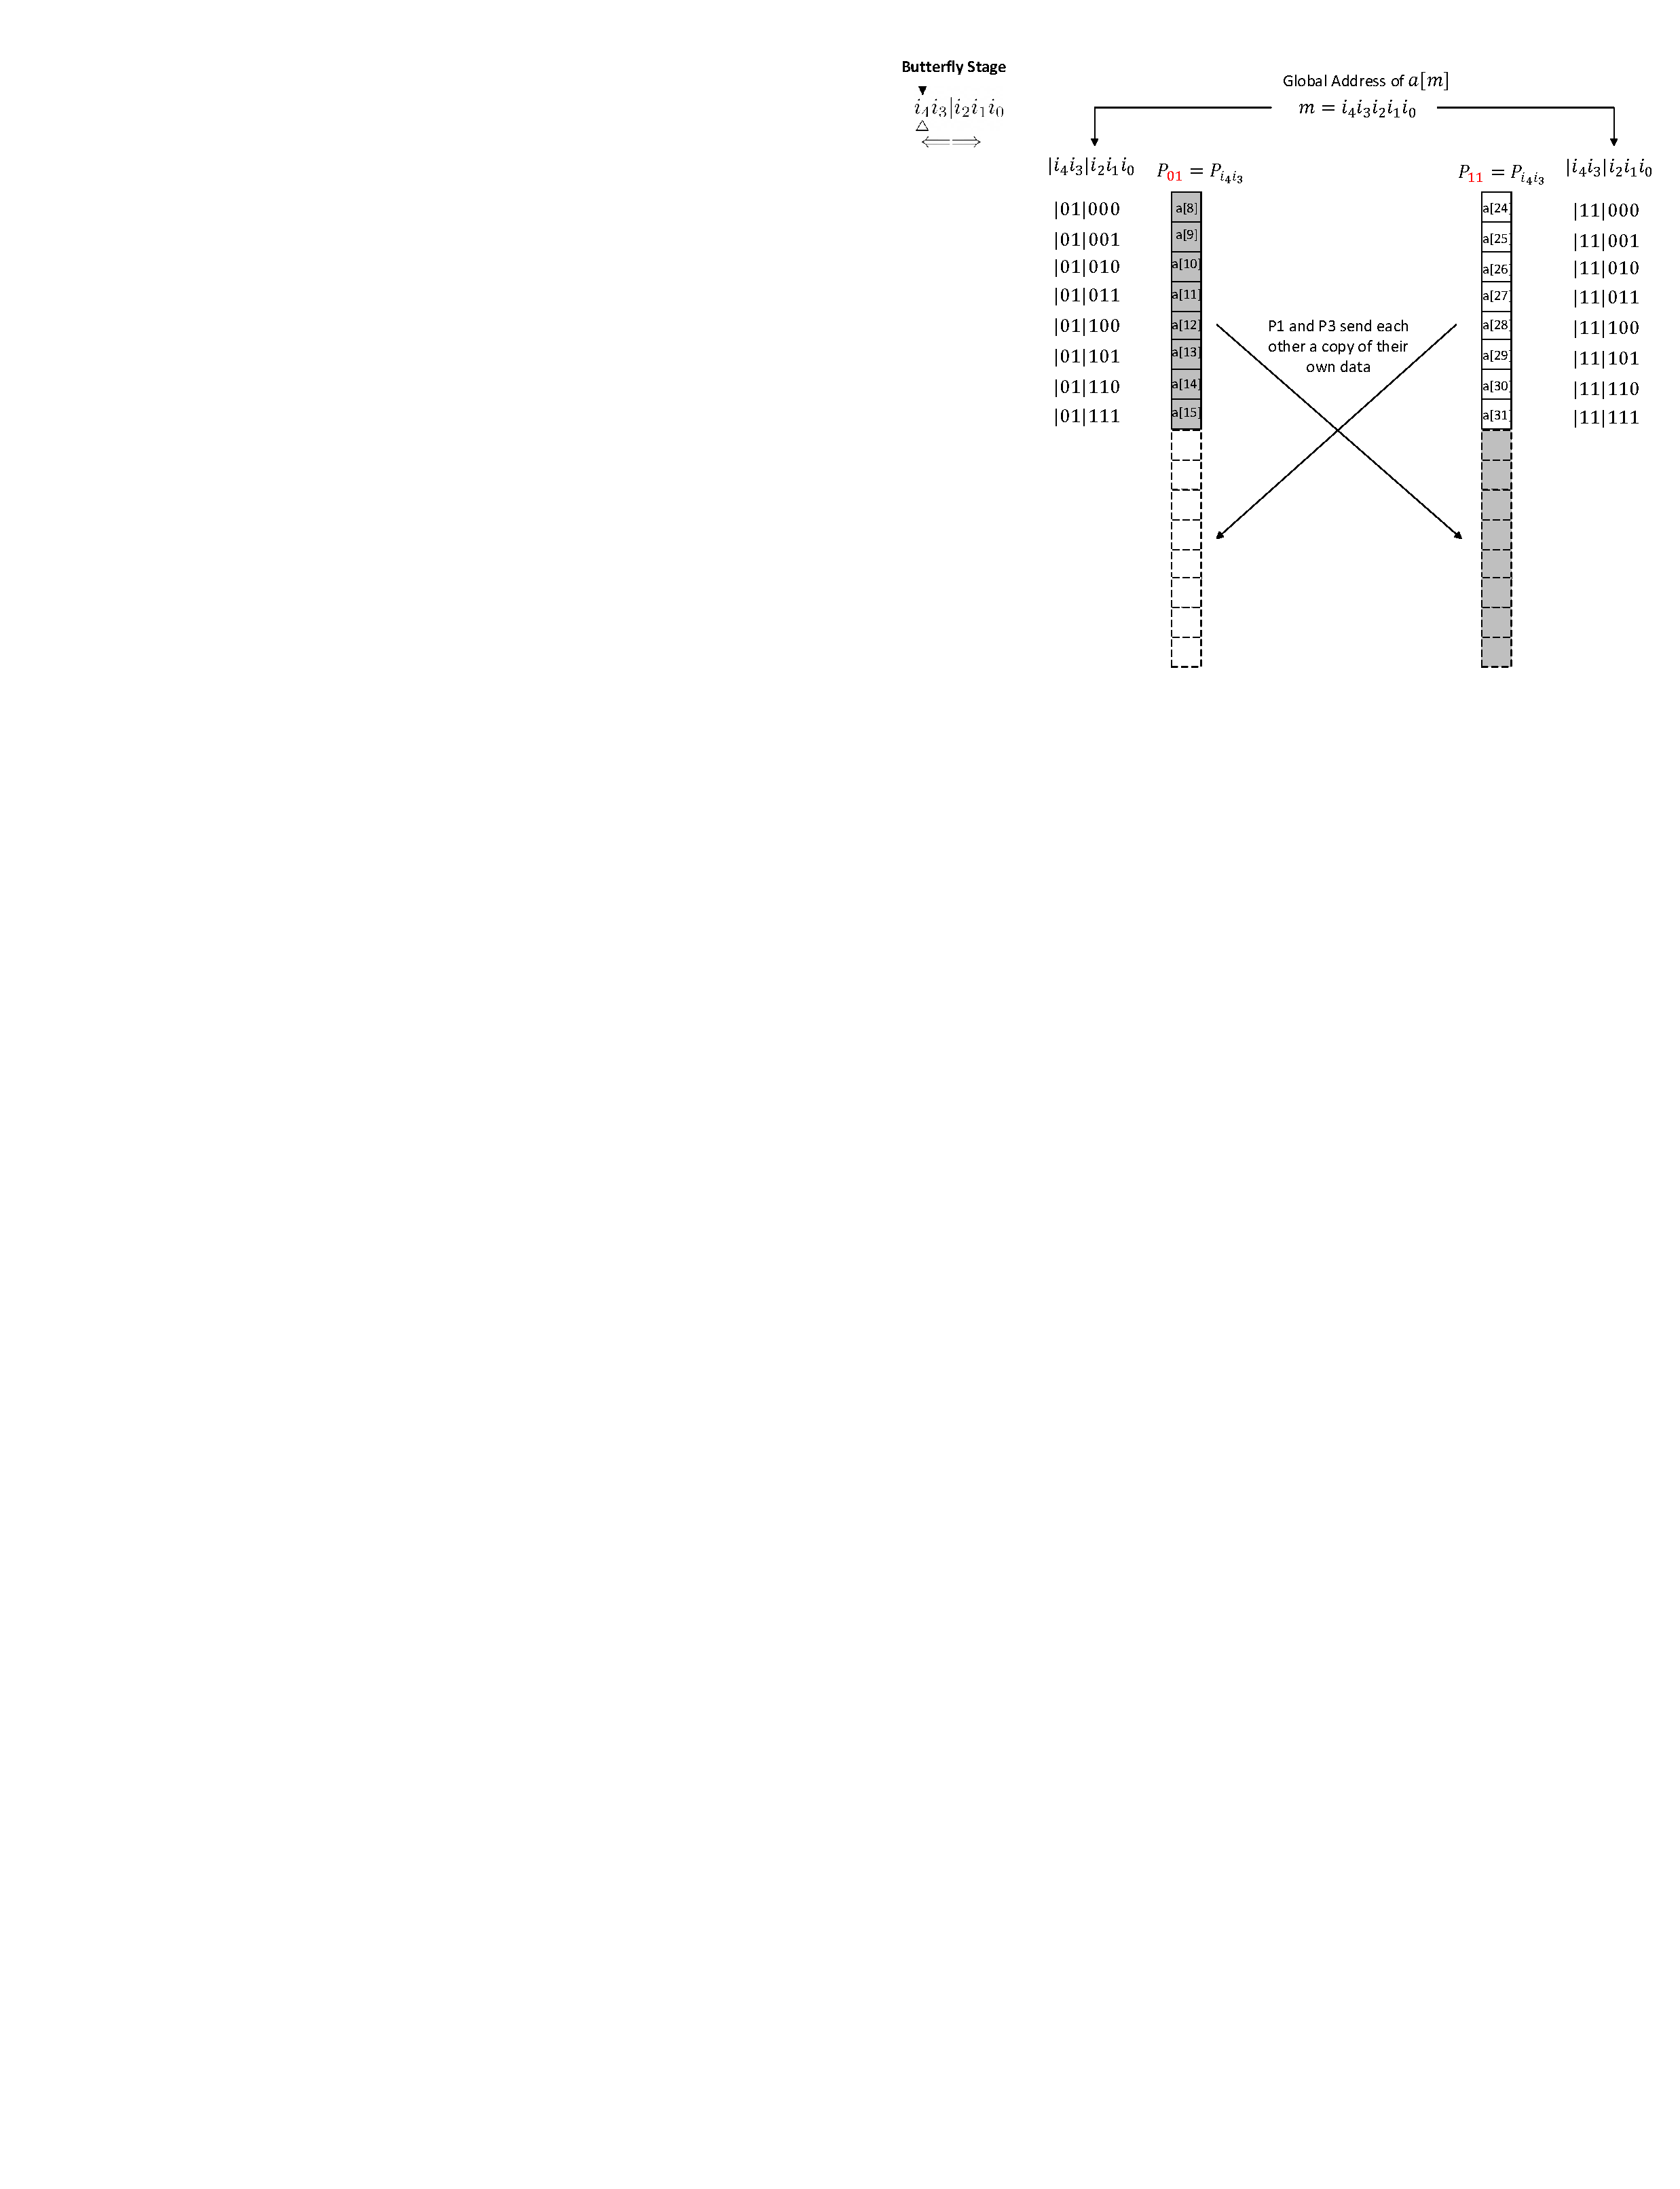
\includegraphics[width=\textwidth]{./fig/DataSwapWithoutPerm2.pdf}
\caption{In round-0, Data sent and received by processors $P_1$ and $P_3$}\label{fig:dataswap_without_perm2}
\end{subfigure}

\begin{subfigure}[b]{0.47\textwidth}
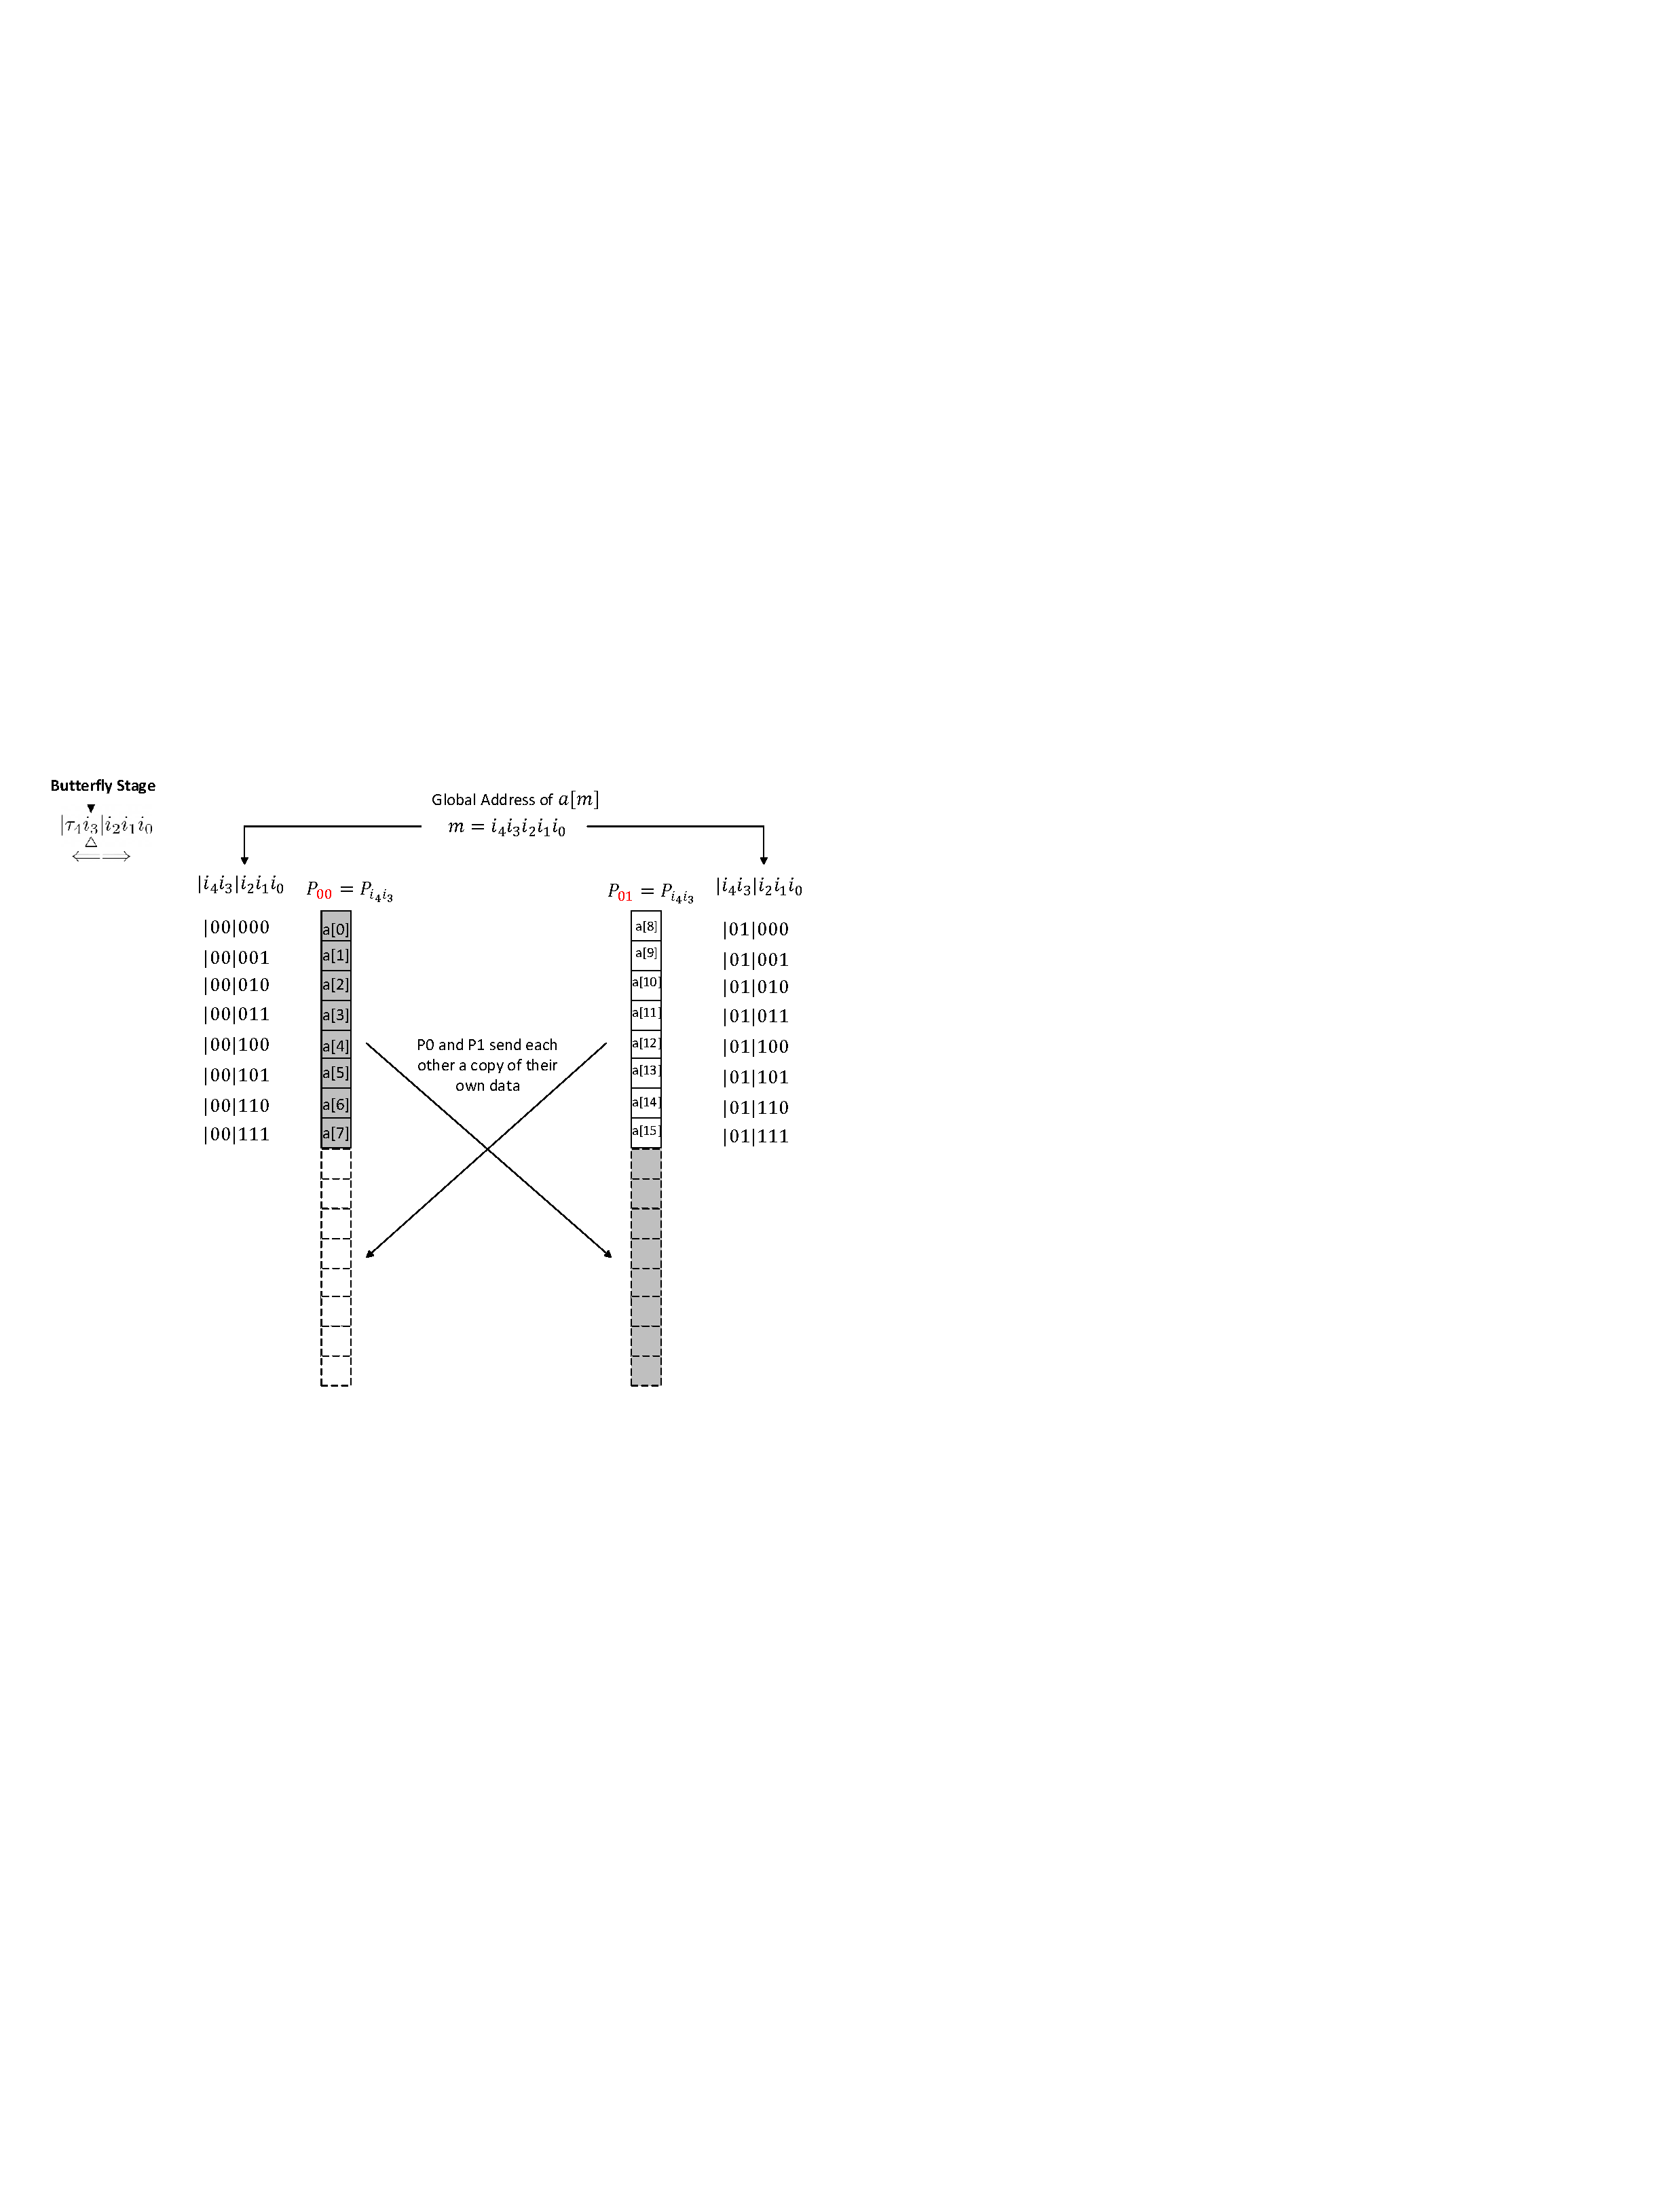
\includegraphics[width=\textwidth]{./fig/DataSwapWithoutPerm3.pdf}
\caption{In round-1, Data sent and received by processors $P_0$ and $P_1$}\label{fig:dataswap_without_perm3}
\end{subfigure}
\hspace{1em}
\begin{subfigure}[b]{.47\textwidth}\centering
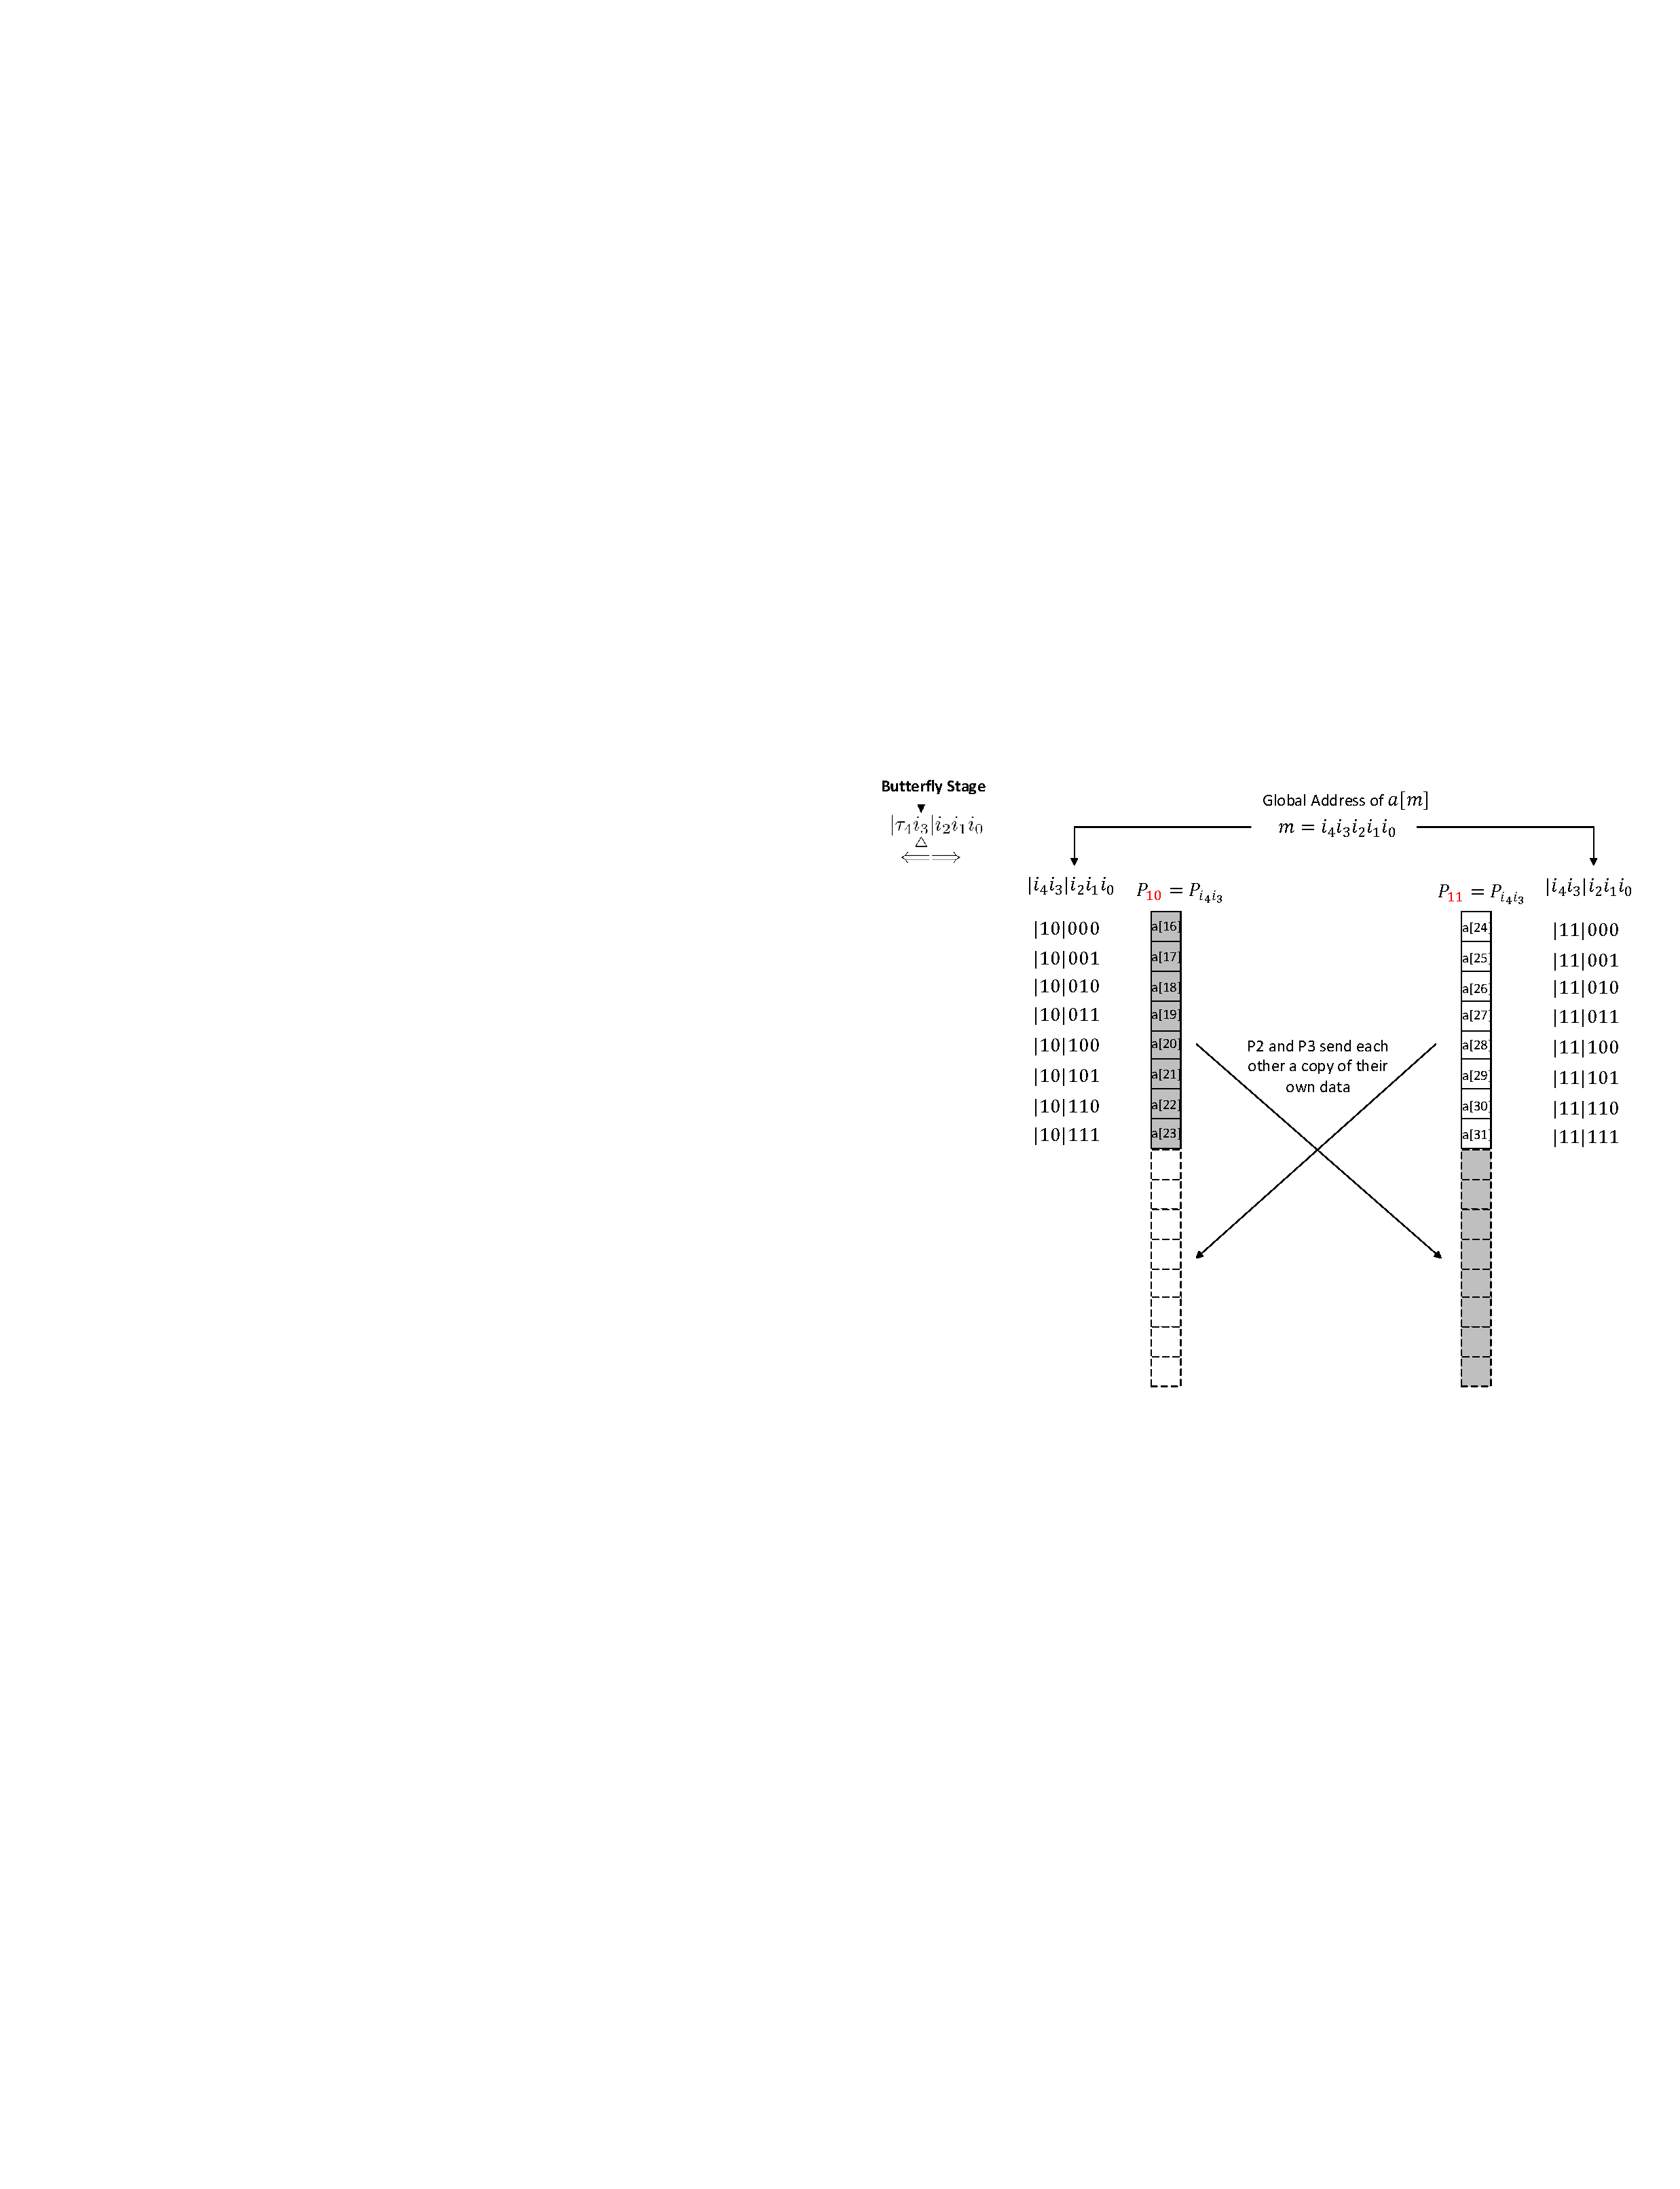
\includegraphics[width=\textwidth]{./fig/DataSwapWithoutPerm4.pdf}
\caption{In round-1, Data sent and received by processors $P_2$ and $P_3$}\label{fig:dataswap_without_perm4}
\end{subfigure}

\caption{An illustrative example for parallelizing in-place NTT($N=32,d=4$) without inter-processor permutations}\label{fig:dataswap_without_perm}
\end{figure*}

\textbf{Remarks} The parallel in-place NTT without inter-processor permutations approach employs \textit{data exchange between a pair of processors}. That is, one processor's initial complement of data may swap with that of another processor. With use of this type of data exchange, $N/d$ butterfly computations are performed in parallel at the cost of a number of $N/d$ data swaps per processor.  


\subsection{Second attempt: Parallel NTTs with Inter-processor permutations}
In this subsection, we discuss the class of parallel NTTs which employ inter-processor data permutations. Similar to the one presented in the previous subsection which evenly distributes all butterfly computations among the processors, the new method also reduces the message length from $\frac{N}{d}$ elements to $\frac{1}{2}\frac{N}{d}$ in each of the $log_2d+1$ concurrent message exchanges.

% \textbf{Modified shorthand notation} The new idea can be explained using a familiar example: suppose that $N=32$, and a consecutive data map denoted by $|i_4i_3|i_2i_1i_0$ is used to distribute data among
% the four processors. A shorthand notation must reflect both the permutation and the computation accomplished in the parallel NTT approach. The modified notation extends the previous notation used for parallel NTT without permutations approach, and represent the first stage of butterfly computation as follows:

% \begin{table}[h!]\begin{center}
% \scalebox{0.8}{\begin{tabular}{c c}
% \hline
% $|i_4i_3|i_2i_1i_0$ & $|\underset{\triangle}{i_2}i_3|\underset{\triangle}{\overset{\blacktriangledown}{i_4}}i_1i_0$\\
% Initial Map   &   $\longleftarrow\longrightarrow$\\
% \hline
% \end{tabular}}
% \end{center}\end{table}





\begin{figure*}[!tb]
\centering
\begin{subfigure}[b]{\textwidth}
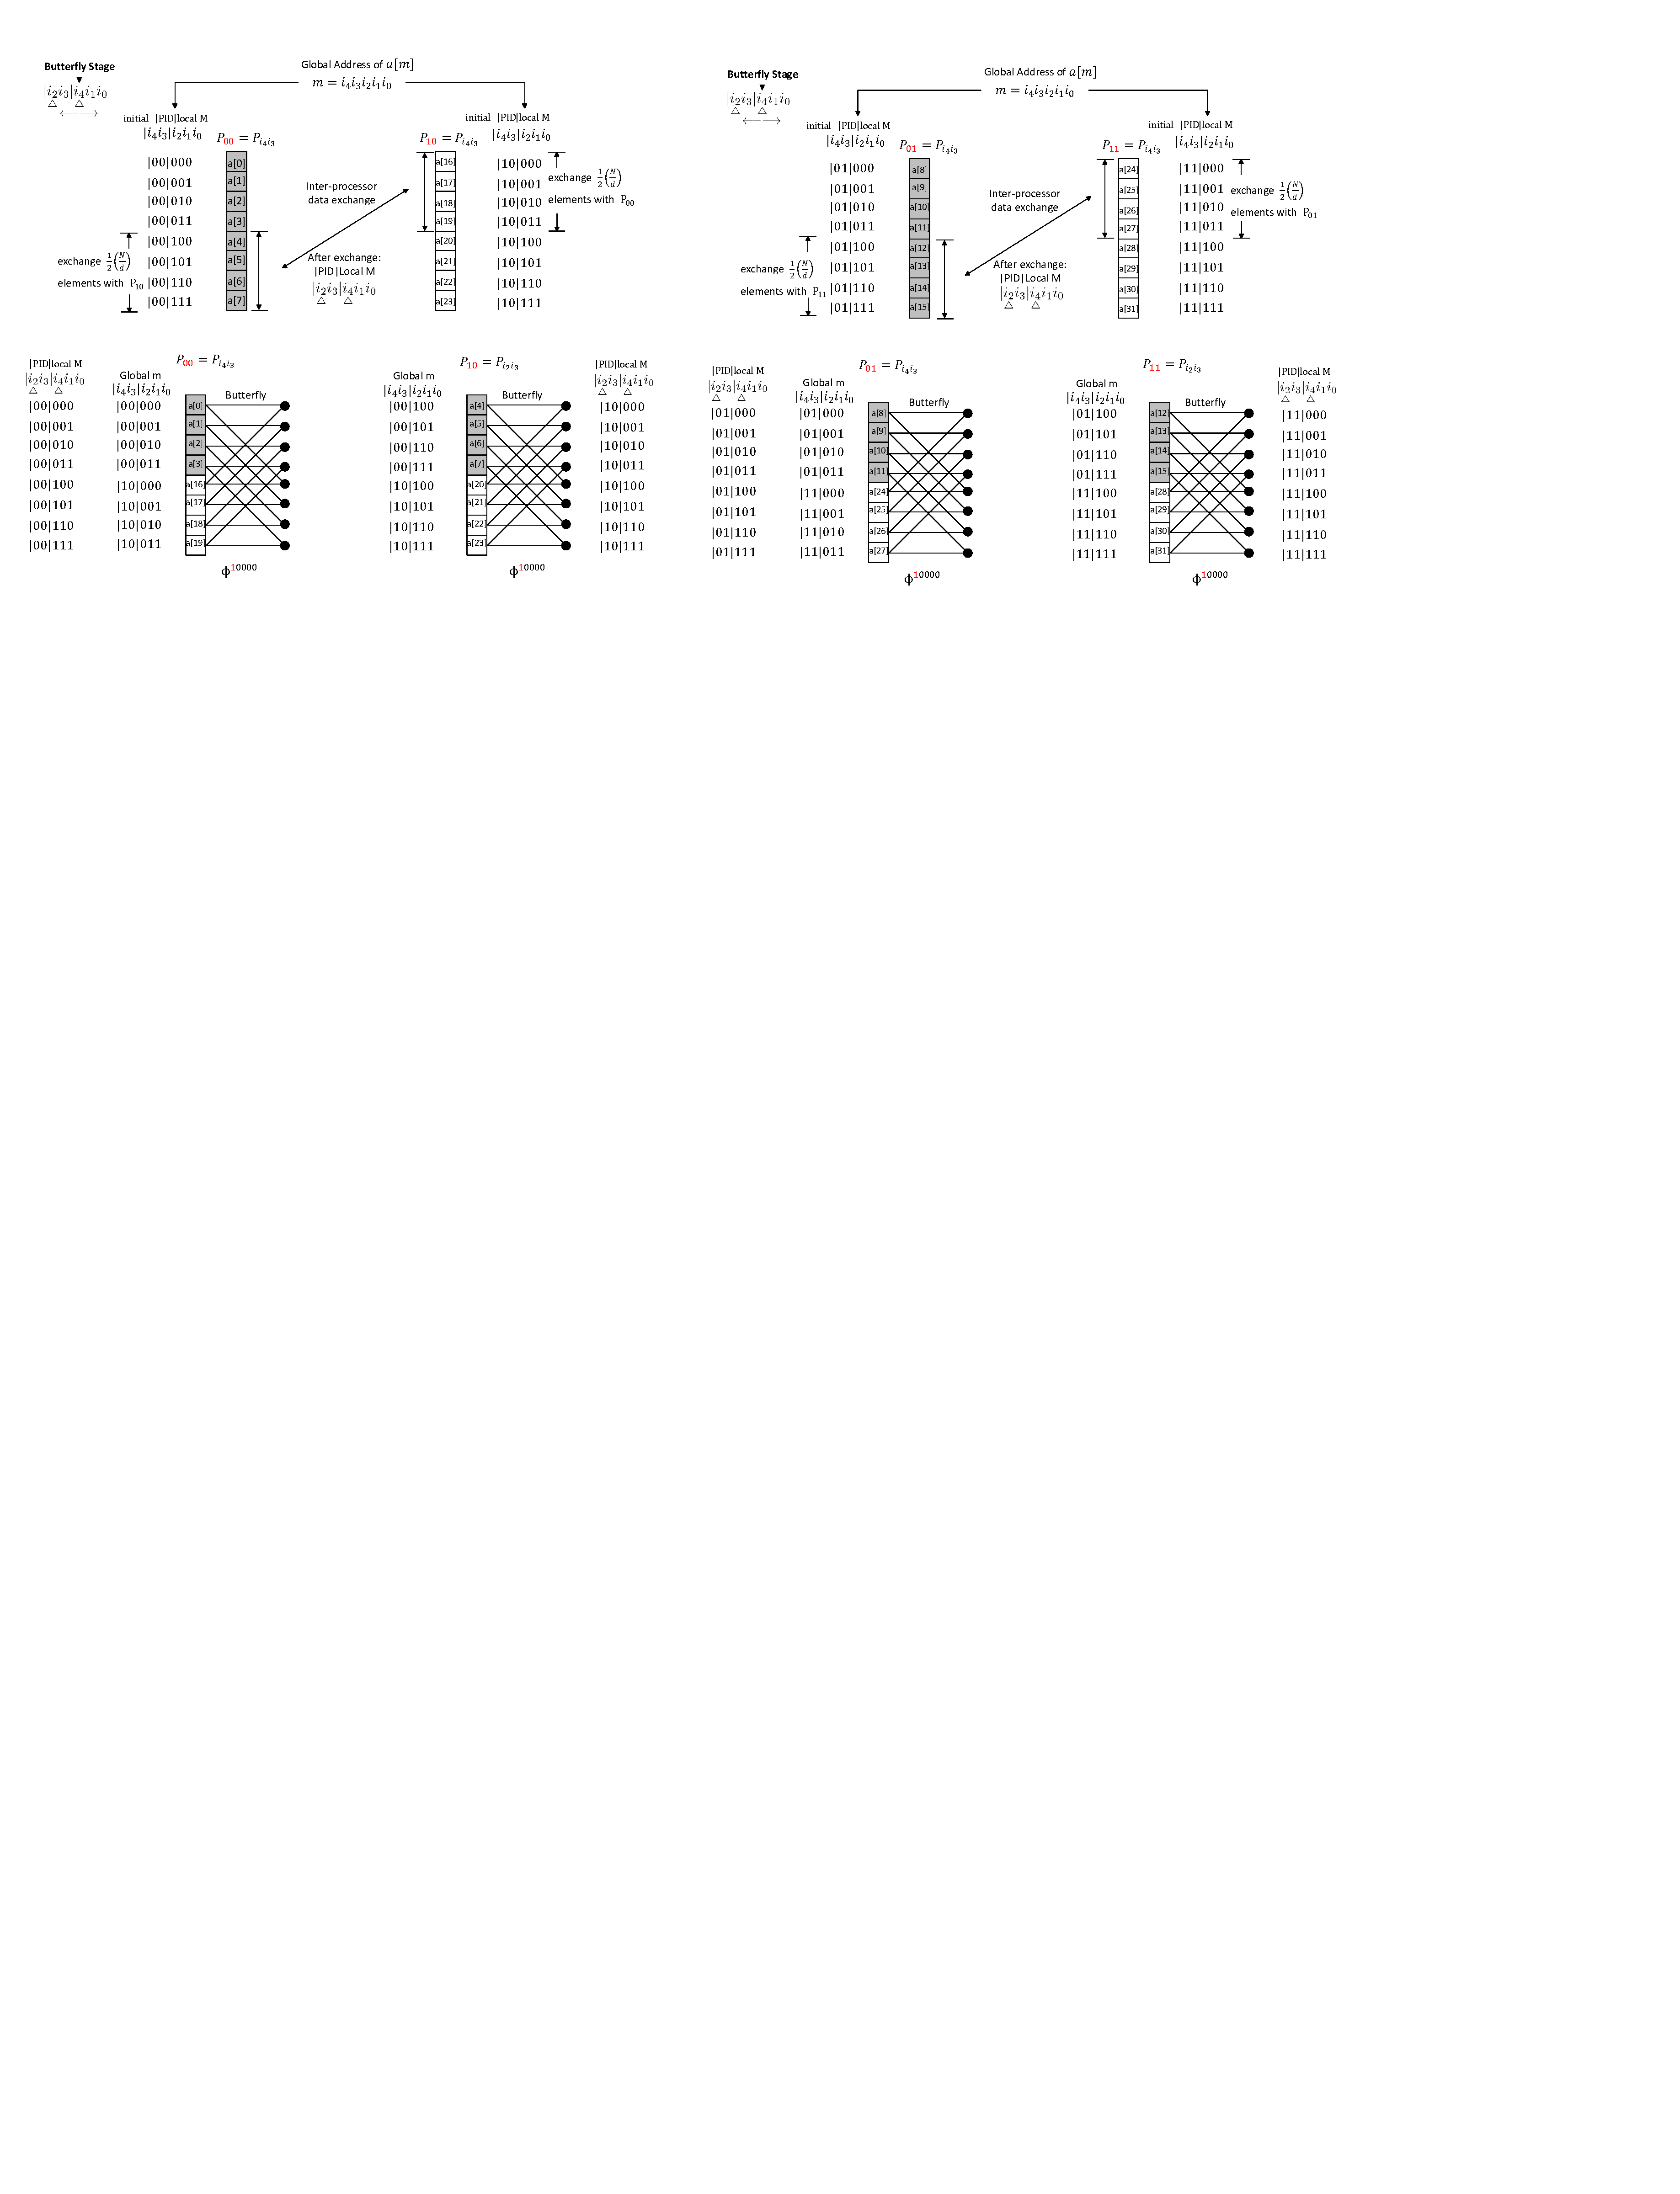
\includegraphics[width=\textwidth]{./fig/DataSwapWithPerm1.pdf}
\caption{In round-0, $DIT_{NR}$ butterfly computation with data migration between processors $P_0$ and $P_2$, and $P_1$ and $P_3$, respectively}\label{fig:dataswap_with_perm1}
\end{subfigure}
\hspace{1em}
\begin{subfigure}[b]{\textwidth}\centering
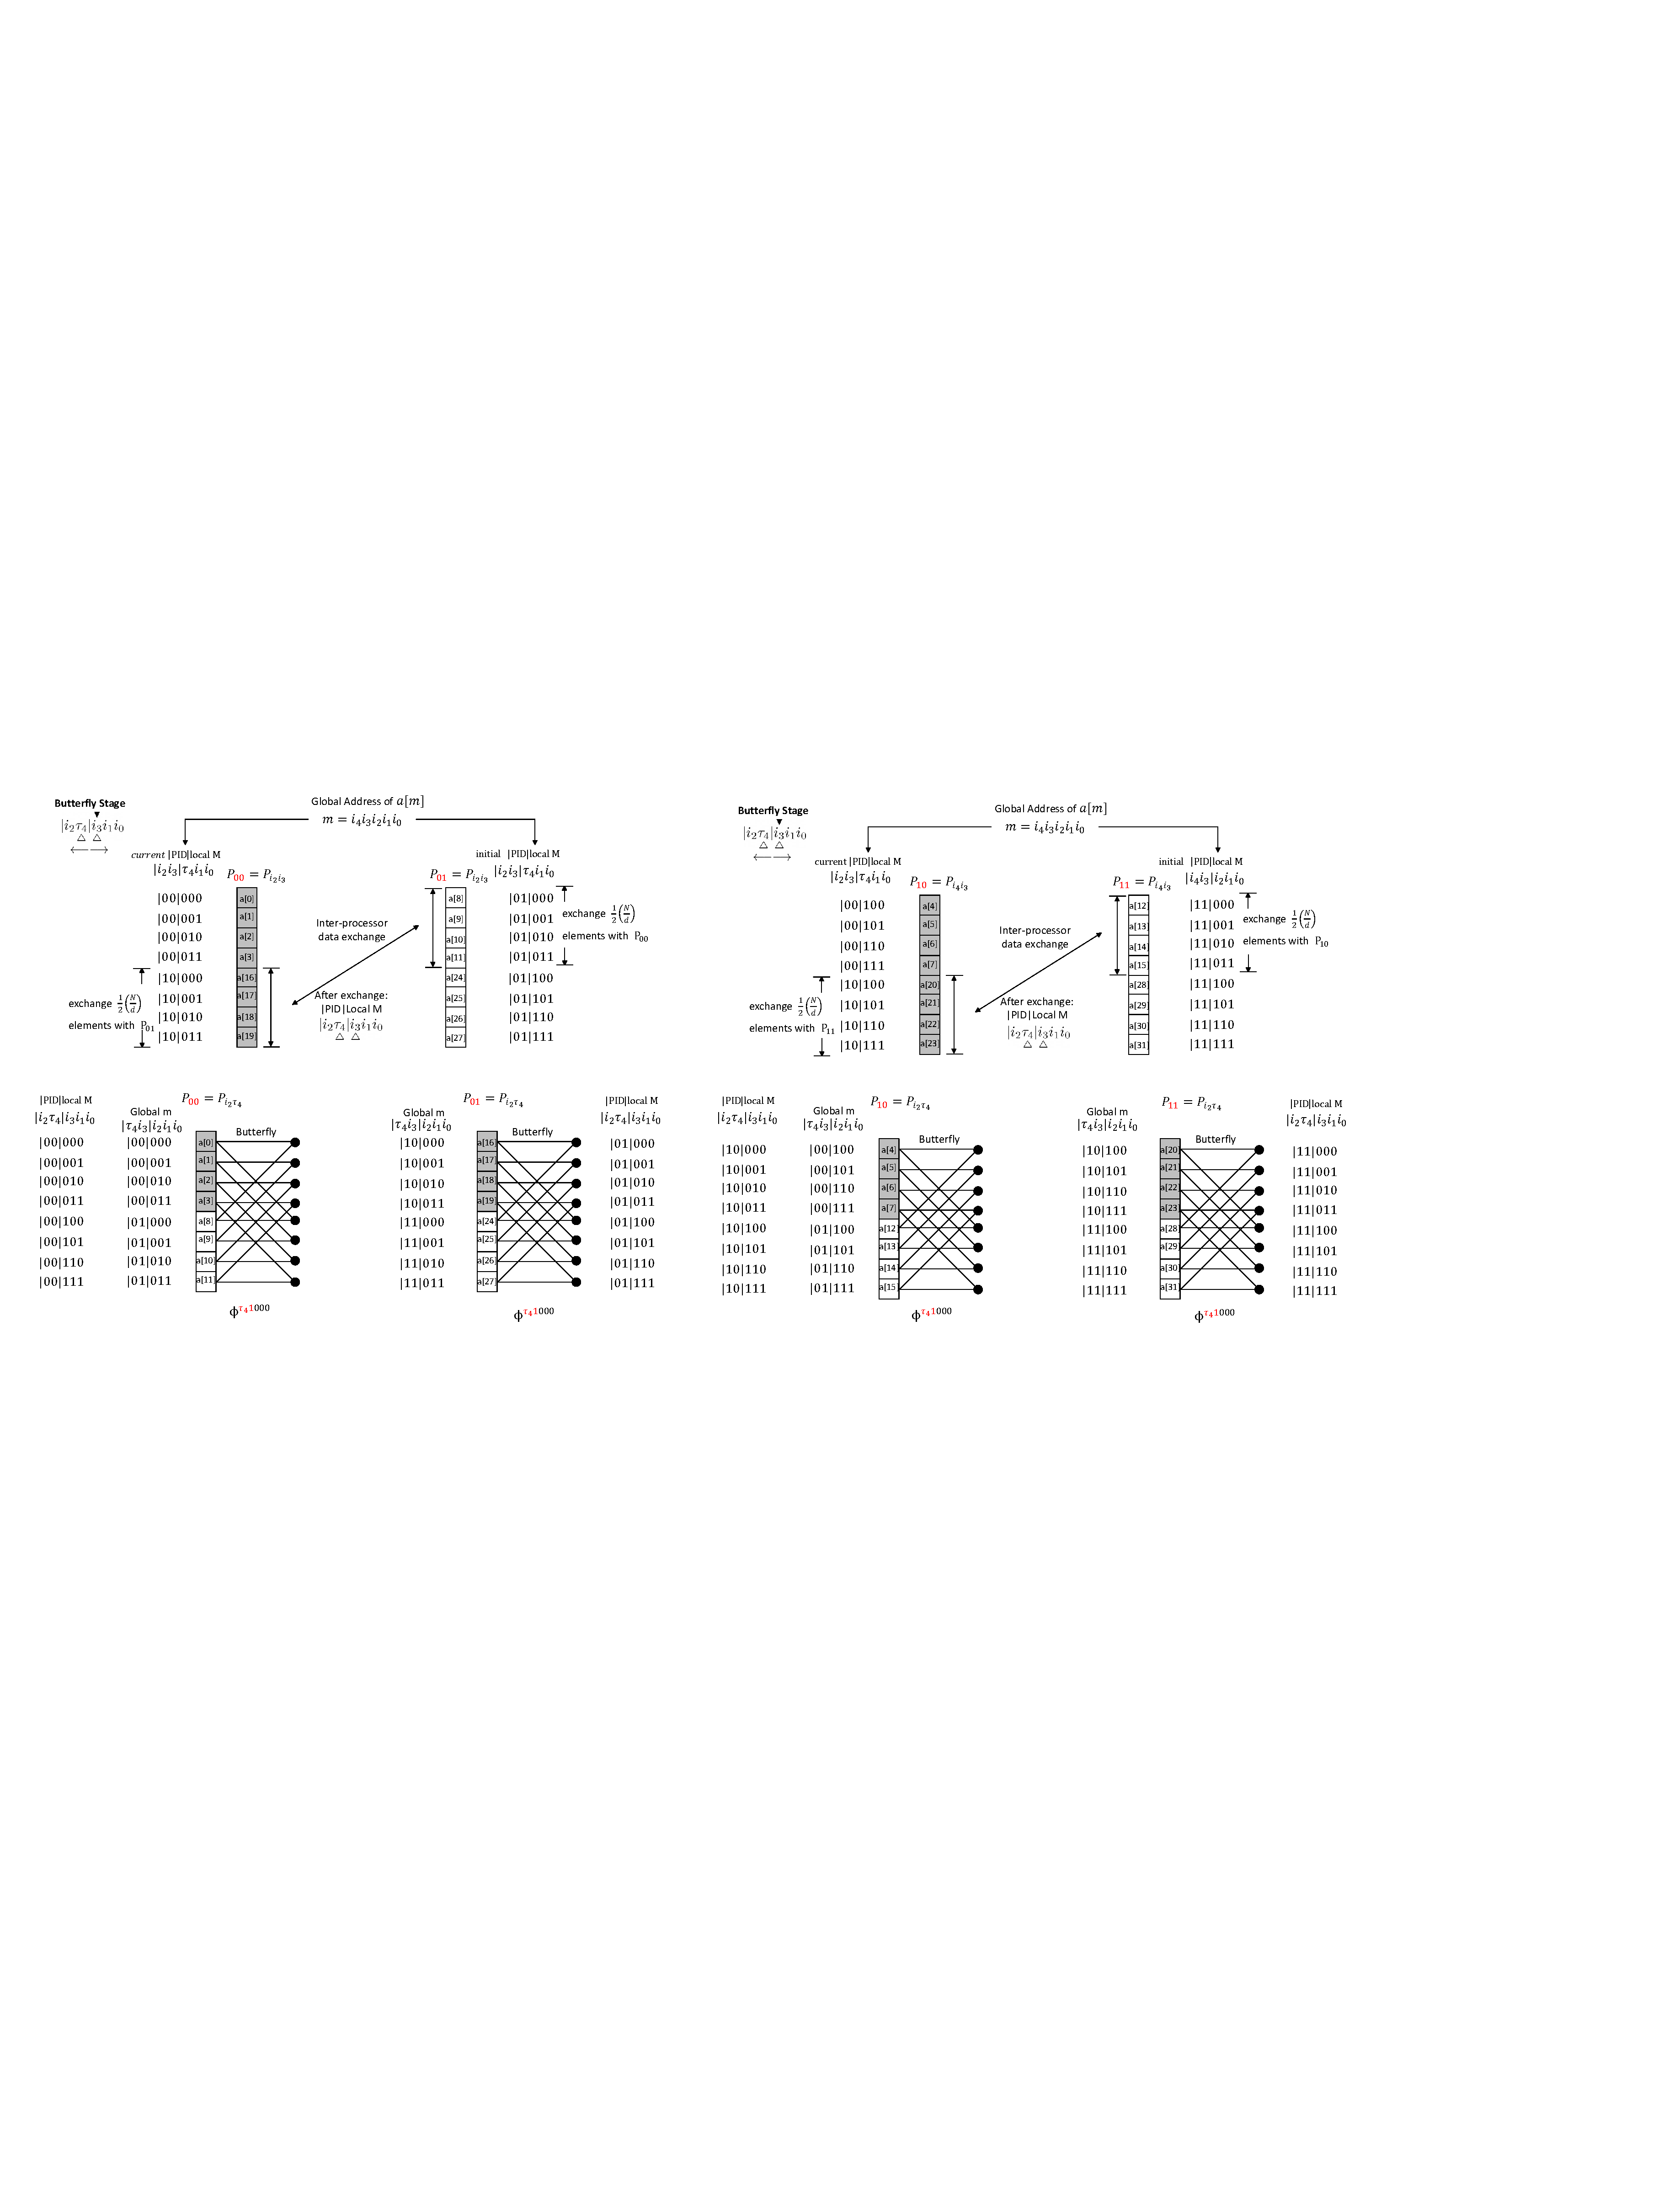
\includegraphics[width=\textwidth]{./fig/DataSwapWithPerm2.pdf}
\caption{In round-1, $DIT_{NR}$ butterfly computation with data migration between processors $P_0$ and $P_1$, and $P_2$ and $P_3$, respectively}\label{fig:dataswap_with_perm2}
\end{subfigure}
\hspace{1em}
\begin{subfigure}[b]{\textwidth}
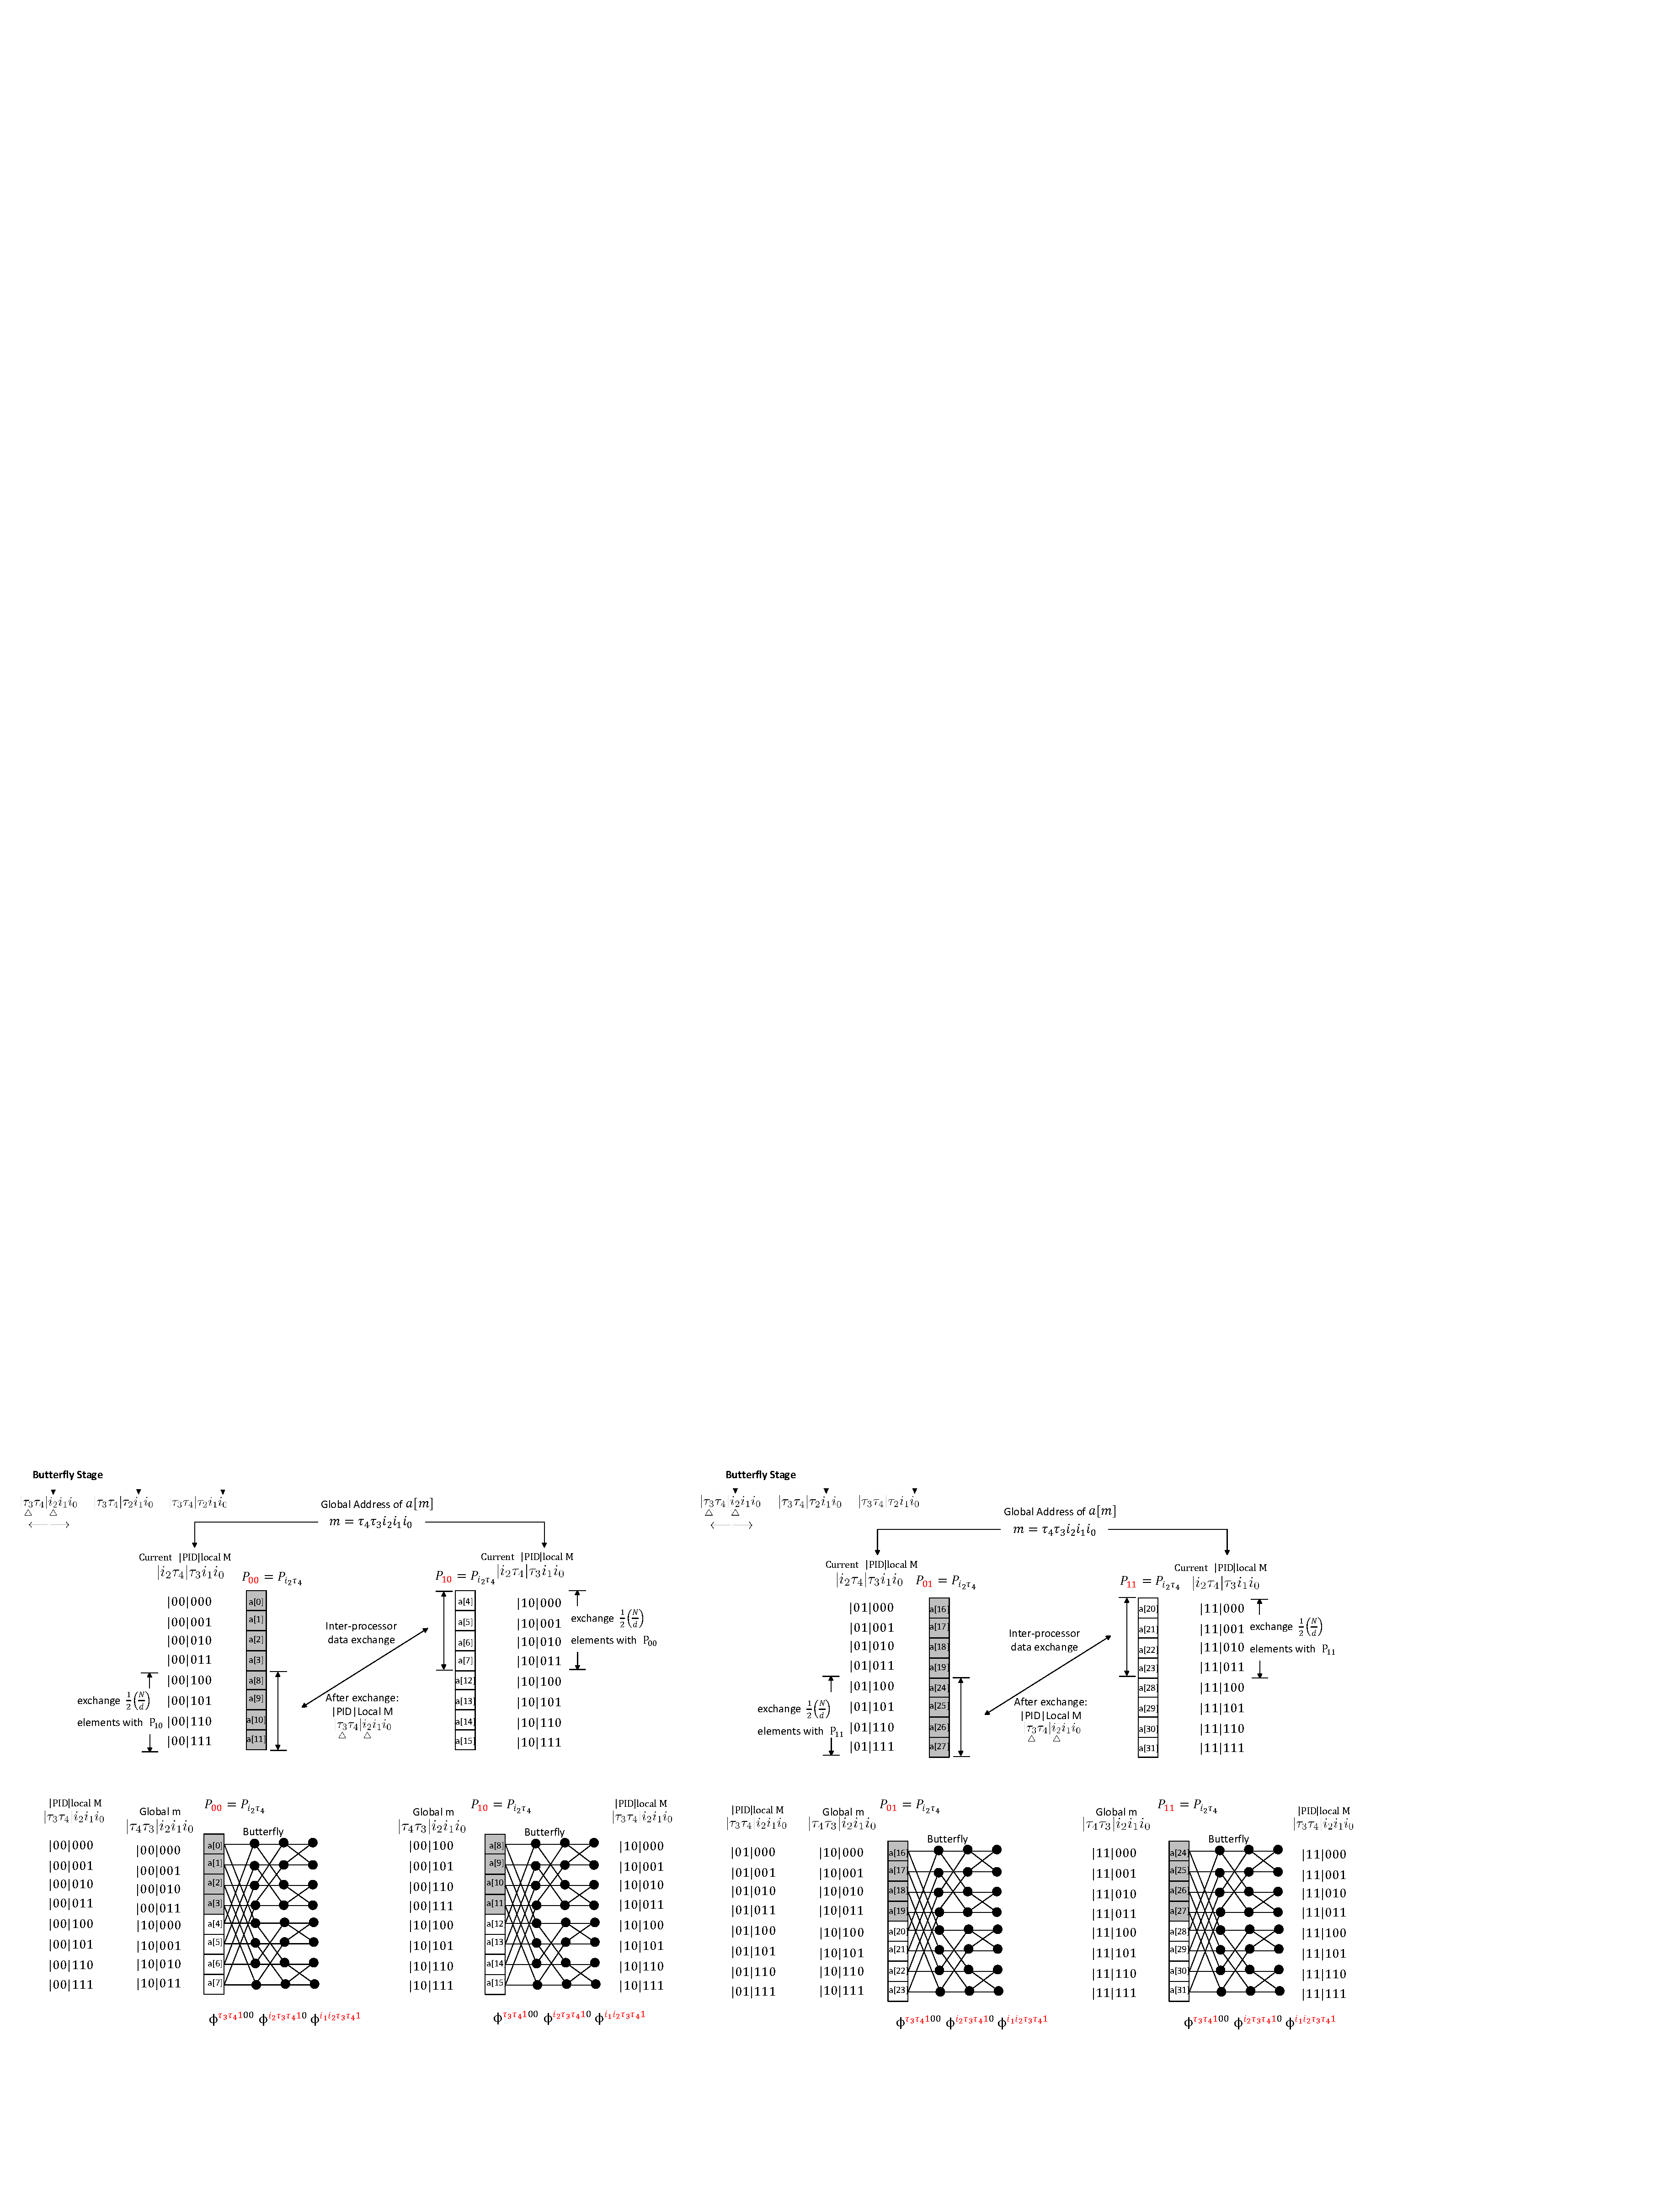
\includegraphics[width=\textwidth]{./fig/DataSwapWithPerm3.pdf}
\caption{In round-2/3/4, $DIT_{NR}$ butterfly computation with data migration between processors $P_0$ and $P_2$, and $P_1$ and $P_3$, respectively}\label{fig:dataswap_with_perm3}
\end{subfigure}
\caption{An illustrative example for parallelizing in-place NTT($N=32,d=4$) with inter-processor permutations}\label{fig:dataswap_with_perm}
\end{figure*}




\textbf{The complete algorithm} We use the shorthand notation we have developed with symbols $\triangle$ and $\blacktriangledown$, the complete parallel algorithm corresponding to $DIT_{NR}$ NTT is represented below for the $N=32$ example.
\begin{table}[h!]\begin{center}
\scalebox{0.8}{\begin{tabular}{c c c c c c}
\hline
$|i_4i_3|i_2i_1i_0$ & $|\underset{\triangle}{i_2}i_3|\overset{\blacktriangledown}{\underset{\triangle}{i_4}}i_1i_0$ & $|i_2\underset{\triangle}{\tau_4}|\overset{\blacktriangledown}{\underset{\triangle}{i_3}}i_1i_0$ & $|\underset{\triangle}{\tau_3}\tau_4|\overset{\blacktriangledown}{\underset{\triangle}{i_2}}i_1i_0$ & $|\tau_3\tau_4|\tau_2\overset{\blacktriangledown}{i_1}i_0$ & $|\tau_3\tau_4|\tau_2\tau_1\overset{\blacktriangledown}{i_0}$\\
Initial Map   &   $\longleftarrow\longrightarrow$ &  $\longleftarrow\longrightarrow$ &  $\longleftarrow\longrightarrow$\\
\hline
\end{tabular}}
\end{center}\end{table}

To provide complete information for this example,  in the initial map (before performing the first stage butterfly computation), the input data are distributed as the element $a_{i_4i_3i_2i_1i_0}$ can be found in $A[i_2i_1i_0]$ in processor $P_{i_4i_3}$. For example, $a[19]=a_{19}$ is shown to be initially in $A[3]$ in $P_2$ and $A[14]=a_{14}$ in $A[6]$ in $P_1$ in Fig.~\ref{fig:dataswap_with_perm1} since $19=10|011_2$ and $14=01|110_2$. 


To prepare data for each processor in the first round of butterfly computation where $P_0$ connects $P_2$ and $P_1$ connects $P_3$ due to the hypercube structure, $P_0$ swaps the  second half of his local array with the first half of $P_2$'s local array, and $P_1$ swaps the second half of his local array with the first half of $P_3$'s local array as dipicted in Fig.~\ref{fig:dataswap_with_perm1}. The symbols $\triangle$ are used to locate the exact position of the element $a_i$ after such data swap: the bit $\underset{\triangle}{i_k}$, which has just been permuted from PID to Local $M$, and the bit $\underset{\triangle}{i_{\ell}}$, which has just been permuted from Local $M$ to the PID. In our case, the notation $|\underset{\triangle}{i_2}i_3|\overset{\blacktriangledown}{\underset{\triangle}{i_4}}i_1i_0$ is used which means bit $i_4$ in the PID and bit $i_2$ in the local $M$ switch their positions in the shorthand notation (denoted by the symbols $\triangle$) making the memory mapping changed to $i_2i_3|i_4i_1i_0$, which means that the data in $a[i_4i_3i_2i_1i_0]$ can now be found in $A[i_4i_1i_0]$ in $P_{i_2i_3}$. For example, $a[19]=a_{19}$ is relocated to $A[7]$  in $P_0$ ($A[7]$ means the 7-th element for $P_0$'s local array) after the inter-processor permutation shown in Fig.~\ref{fig:dataswap_with_perm1} since $10|011_2$ is changed to $00|111_2$; $a[14]=a_{14}$ is relocated to $A[2]$ in $P_3$ after the inter-processor permutation shown in Fig.~\ref{fig:dataswap_with_perm1} since $01|110_2$ is changed to $11|010_2$. After the memory swap, all data are located correctly in the corresponding processors to perfom the first round of butter fly computation. The symbol $\blacktriangledown$ is used to indicate the pairs of elements for the butterfly computation in each processor, \textit{i.e.},
$|\underset{\triangle}{i_2}i_3|\overset{\blacktriangledown}{\underset{\triangle}{i_4}}i_1i_0$ means $A[i_2i_30i_1i_0]$ should pair with $A[i_2i_31i_1i_0]$ to complete elementary butterfly unit computation for $P_{i_2i_3}$. Also, the index $i_k$ that the symbol $\blacktriangledown$ points to is changed to $\tau_k$ for showing that this particular round of butterfly computation is completed. A  quick observation is that there are $i-1$ indices changed to $\tau$ in the notation for the $i$-th round of computation: for example, $|\underset{\triangle}{i_2}i_3|\overset{\blacktriangledown}{\underset{\triangle}{i_4}}i_1i_0$ represents the first round where no $\tau$ indices exist; $|i_2\underset{\triangle}{\tau_4}|\overset{\blacktriangledown}{\underset{\triangle}{i_3}}i_1i_0$ represents the second round where one $\tau$ index ($i_4$ changed to $\tau_4$) exists and \textit{etc}.


For the second round of butterfly computation where $P_0$ connects $P_1$ and $P_2$ connects $P_3$, $P_0$ swaps the second half of his array with the first half of $P_1$'s local array, and $P_2$ swaps the second half of his local array with the first half of $P_3$'s local array as dipicted in Fig.~\ref{fig:dataswap_with_perm2}.  a similar notation $|i_2\underset{\triangle}{\tau_4}|\overset{\blacktriangledown}{\underset{\triangle}{i_3}}i_1i_0$ is used to denote the memory swap: bit $\tau_4$ in the PID and bit $i_3$ in the local $M$ switch their positions in the shorthand notation making the memory mapping changed from previous $i_2i_3|i_4i_1i_0$ to $i_2i_4|i_3i_1i_0$. For example, $a_{19}$ which is previously stored in $A[7]$ from $P_0$ is now changed to $A[3]$ from $P_1$ since $19=10|011_2$ is rearranged to $01|011_2$. Moreover, $A[i_2i_40i_1i_0]$ pairs with $A[i_2i_41i_1i_0]$ to complete elementary butterfly unit computation for $P_{i_2i_4}$ for all $i_2,i_4,i_1,i_0$. 

For the third round of butterfly computation where $P_0$ connects $P_2$ and $P_1$ connects $P_3$, $P_0$ swaps the  second half of his local array with the first half of $P_2$'s local array, and $P_1$ swaps the second half of his local array with the first half of $P_3$'s local array as dipicted in Fig.~\ref{fig:dataswap_with_perm3}. This swapping pattern is captured in the notation $|\underset{\triangle}{\tau_3}\tau_4|\overset{\blacktriangledown}{\underset{\triangle}{i_2}}i_1i_0$ indicating the previous $i_2i_4|i_3i_1i_0$ is changed to $i_3i_4|i_2i_1i_0$ due to the $\triangle$ annotations. For example, $a_{19}$ which is previously stored in $A[3]$ from $P_1$ is still preserved in $A[3]$, $P_1$ since $19=10|011_2$ is rearranged to $01|011_2$. The $\blacktriangledown$ annotation indicates that $A[i_3i_40i_1i_0]$ pairs with $A[i_3i_41i_1i_0]$ to complete elementary butterfly unit computation for $P_{i_3i_4}$ for all $i_3,i_4,i_1,i_0$.

There are no inter-processor data swapping for the last two rounds, \textit{i.e.}, the fourth and the fifth round of butterfly computation. However, the $\blacktriangledown$ annotation helps distinguish which two data elements should pair to complete the elementary butterfly unit computation inside the processor: in the fourth round, $A[i_3i_4i_20i_0]$ pairs with $A[i_3i_4i_21i_0]$ for $P_{i_3i_4}$, and in the fifth round, $A[i_3i_4i_2i_10]$ pairs with $A[i_3i_4i_2i_11]$ for $P_{i_3i_4}$. The computations in the fourth and fifth round are merged to Fig.~\ref{fig:dataswap_with_perm3}.




After all five rounds of butterfly computation are completed, the NTT results are stored in the array $a[\cdot]$ but the position is rearranged: the output data element $A_{i_0i_1i_2i_3i_4}$, which overwrites the data in $a[i_4i_3i_2i_1i_0]$, is finally contained in $A[i_2i_1i_0]$ in $P_{i_3i_4}$. Such arrangement for the data mapping for the output elements is observed as following:

\begin{itemize}
    \item The \textit{in-place} butterfly computation in the $DIT_{NR}$ algorithm ensures $a[i_4i_3i_2i_1i_0]=a_{i_4i_3i_2i_1i_0}^{(5)}=A_{i_0i_1i_2i_3i_4}$ where $A_{i_0i_1i_2i_3i_4}=\sum_j a_j(\omega_{N}^{i_0i_1i_2i_3i_4}\cdot\omega_{2N}^1)^j$
    \item The final mapping $|\tau_3\tau_4|\tau_2\tau_1\tau_0$ indicates that the final content in $a[i_4i_3i_2i_1i_0]$ is now located in $a[i_2i_1i_0]$ in processor $P_{i_3i_4}$ (rather than the initially assigned processor $P_{i_4i_3}$)
\end{itemize}


For example, $P_0$ has stored $a[0]-a[7]$ where $a[0]$ computes $A[0]$, $a[1]$ computes $A[16]$, and \textit{etc.}; $P_1$ has stored $a[16]-a[23]$ where $a[16]$ computes $A[1]$, $a[17]$ computes $A[17]$, and \textit{etc.}; $P_2$ has stored $a[8]-a[15]$ where $a[8]$ computes $A[2]$, $a[9]$ computes $A[18]$, and \textit{etc.}; $P_3$ has stored $a[24]-a[31]$ where $a[24]$ computes $A[3]$, $a[25]$ computes $A[19]$, and \textit{etc.}

\textbf{Remarks on the correctness of the notation} Because $i_k$ was in PID session before the switch, $i_k=1$ in one processor, and $i_k=0$ in the other processor. On the other hand, because $i_{\ell}$ was in Local $M$ session before the switch, $i_{\ell}=0$ for half of the data, and $i_{\ell}=1$ for another half of the data. Consequently, the value of $i_k$, the PID bit, is equal to $i_{\ell}$, the local $M$ bit, for half of the data elements in each processor, and the notation which represents the switch of these two bits identifies both the PID of the other processor as well as the data to be sent out or received. To depict exactly what happens, the data exchange between two processors and the butterfly computation represented by $|\underset{\triangle}{i_2}i_3|\underset{\triangle}{\overset{\blacktriangledown}{i_4}}i_1i_0$ is shown in its entirety in Fig.~\ref{fig:dataswap_with_perm1} and \ref{fig:dataswap_with_perm2}.


\begin{algorithm}[!tbh]
 \DontPrintSemicolon % Some LaTeX compilers require you to use \dontprintsemicolon instead
 \KwIn{a polynomial ring $R_q$, and NTT points $N$, input $\mathbf{a} = (a[0],\cdots, a[N-1])$}
 \KwOut{$NTT(\mathbf{a}))=\mathbf{A}=(A[0],\cdots,A[N-1])$}
    Initialize the hypercube connections between $d$ processors as described in Alg.~\ref{alg:descript_hypercube}\;
    Initialize the merged twiddle factor look-up table $\{w_i\}$ as described in Alg.~\ref{alg:descript_twiddlefactor}\;
    /*arrange the data array $a[\cdot]$ in natural order*/\;
    Initialize the data $a[i_{log_2N-log_2d-1}\cdots i_1i_0]$ in $P_{i_{log_2N-1}\cdots i_{log_2N-log_2d}}$ with $a[i_{log_2N-1}\cdots i_1i_0]$ for all $i_{log_2N-1},\cdots,i_0$\;
    /*perform the first $log_2d+1$ round of computations where inter-processor data swapping is required*/\;
    \For{$j\leftarrow 0$ \KwTo $log_2d$}{ 
        \If{$j\neq log_2d$}{
            exchange the first half of data in  $P_{i_{log_2N-1}\cdots i_{log_2N-1-j}\cdots i_{log_2N-log_2d}}$ w.r.t. $i_{log_2N-1-j}=0$ with the second half of data in  $P_{i_{log_2N-1}\cdots i_{log_2N-1-j}\cdots i_{log_2N-log_2d}}$ w.r.t. $i_{log_2N-1-j}=1$\;
        }
        \Else{
            exchange the first half of data in  $P_{i_{log_2N-1}\cdots i_{log_2N-1-j}\cdots i_{log_2N-log_2d}}$ w.r.t. $i_{log_2N-1}=0$ with the second half of data in  $P_{i_{log_2N-1}\cdots i_{log_2N-1-j}\cdots i_{log_2N-log_2d}}$ w.r.t. $i_{log_2N-1}=1$\;
        }
        
        perform within each processor $P_{i_{log_2N-1}\cdots i_{log_2N-1-j}\cdots i_{log_2N-log_2d}}$ the $\frac{N}{2d}$ butterfly computations (round-$j$ butterfly)\;
    }
    /*perform the first $log_2N-log_2d-1$ round of computations where inter-processor data swapping is not required*/\;
    \For{$j\leftarrow log_2d+1$ \KwTo $log_2N-1$}{ 
        perform within each processor $P_{i_{log_2N-1}\cdots i_{log_2N-1-j}\cdots i_{log_2N-log_2d}}$ the $\frac{N}{2d}$ butterfly computations (round-$j$ butterfly)\;
    }
    \Return {the data in all $d$ processors as $\mathbf{A}$\;}
 \caption{Parallel Hypercube NTT}\label{alg:descript_hypercube_ntt}
\end{algorithm}

\textbf{Twiddle Factor LUT Distribution} Let us discuss in details on the distribution of the twiddle factor LUT within each butterfly processor here. In the first $log d+1$ rounds of butterfly computations, memory swapping occurs and each butterfly processor utilizes only $1$ twiddle factor; in the next $logN-logd-1$ rounds, no memory swapping occurs and the number of twiddle factors utilized in eah butterfly processor increases exponentially (starting with $2$). Therefore, the total number of twiddle factors (the depth of twiddle factor LUT) in each processor is:
\[
    \sum_{i=1}^{logd+1}1 + \sum_{i=1}^{logN-logd-1}2^i=\frac{N}{d}+logd-1
\]

A concrete example for the twiddle factor LUT distribution can also be found in Fig~\ref{fig:dataswap_with_perm}. In the first $3$ rounds, each processor uses only $1$ twiddle factor, \textit{i.e.}, $\Phi^{10000}$ where $\Phi$ denotes the $2N$-th primitive root of unity $\omega_{2N}$. In the $4$-th round, each processor uses $2$ twiddle factors, \textit{i.e.}, $\Phi^{\tau_41000}$ for $\tau_4\in\{0,1\}$. In the $5$-th round, each processor uses $4$ twiddle factors, \textit{i.e.}, $\Phi^{\tau_3\tau_4100}$ for $\tau_4\in\{0,1\}, \tau_3\in\{0,1\}$.  Therefore, each processor stores $1+2+4=7$ twiddle factors for the proposed hypercube NTT architecture.



\subsection{Butterfly Processor}\label{sec:butterfly processor}
\begin{figure*}[!tb]
\centering
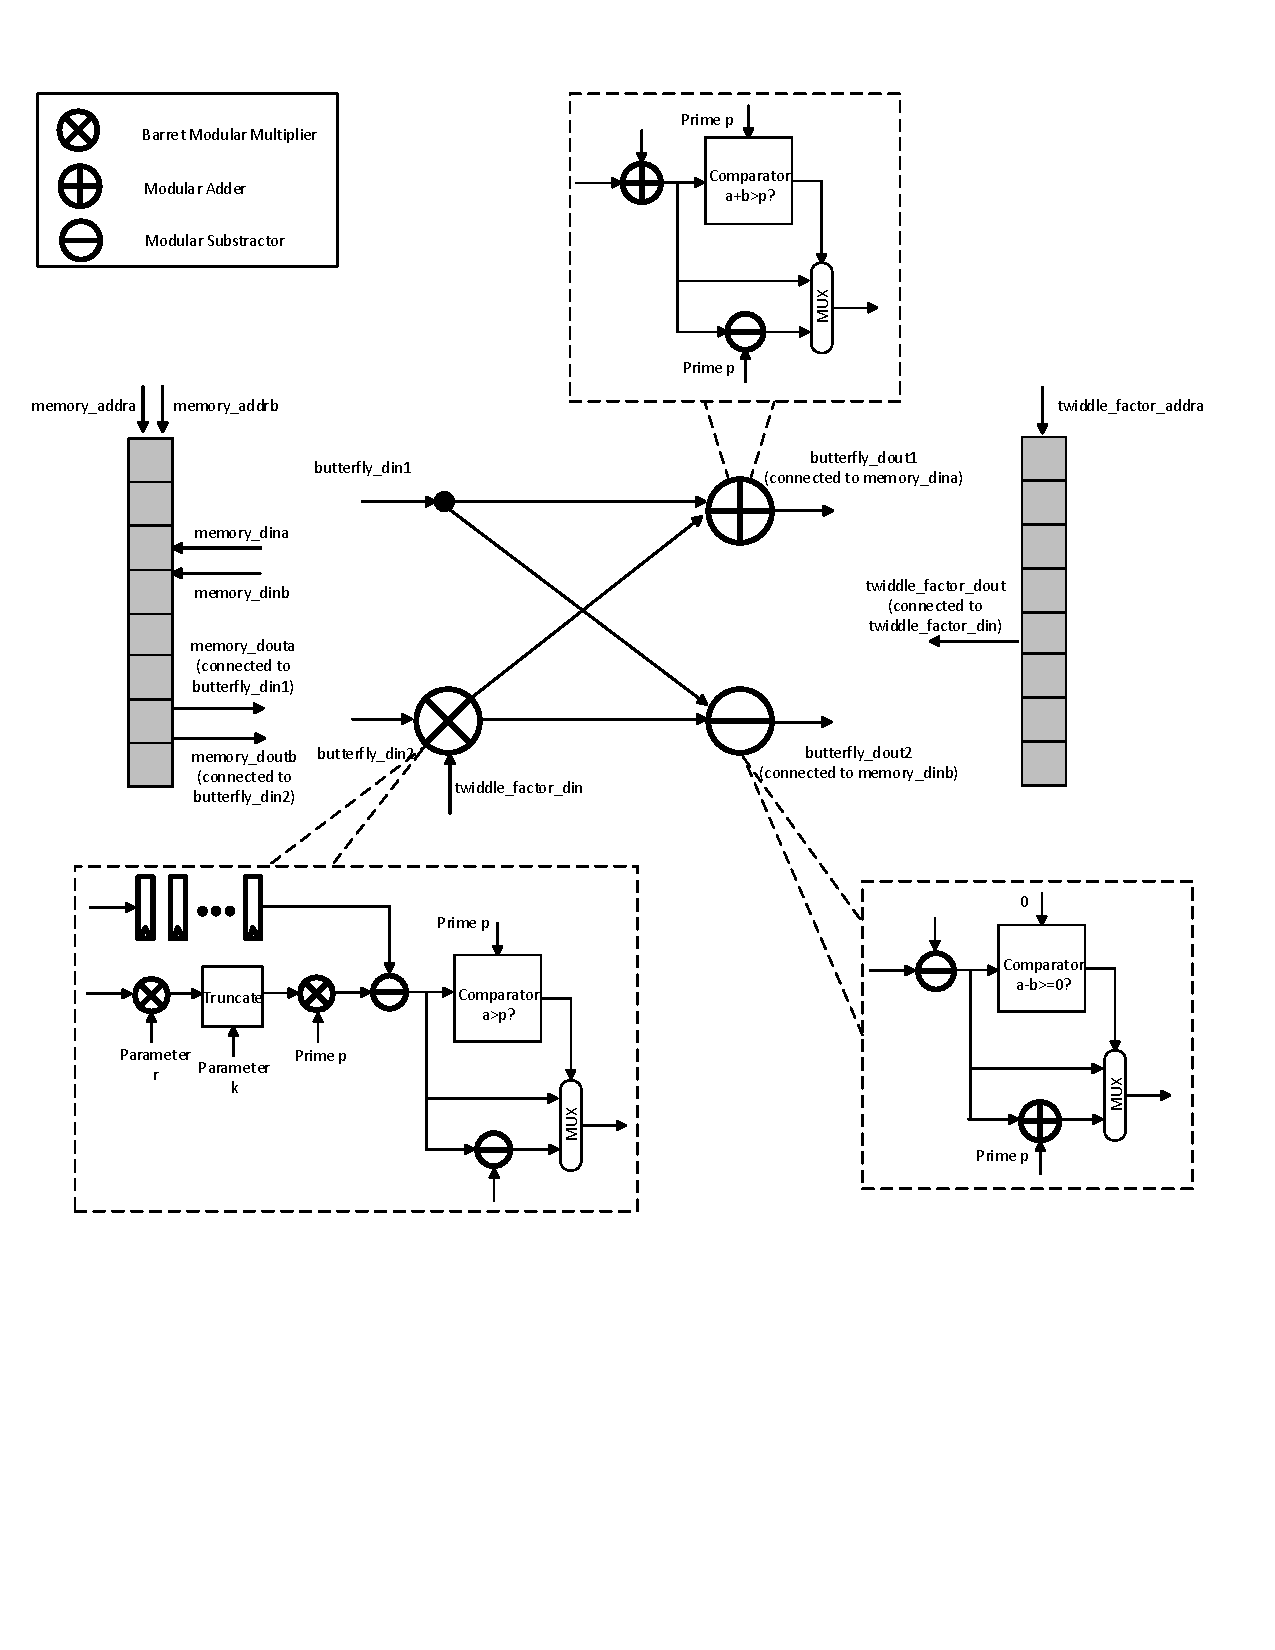
\includegraphics[width=\textwidth]{./fig/processor.pdf}
\caption{Internal structure of butterfly processor}\label{fig:butterfly_processor}
\end{figure*}




\textbf{Design Overview} To perform the butterfly computations and related memory access in each processor efficiently as illustrated in Fig.~\ref{fig:dataswap_with_perm}, a butterfly processor architecture is proposed. Fig.~\ref{fig:butterfly_processor} depicts the internal structure of the butterfly processor. Two memory blocks are instantiated: one dual-port RAM for the $\frac{N}{d}$ points, namely $a_{\frac{N}{d}\cdot i}-a_{\frac{N}{d}\cdot i+\frac{N}{d}-1}$ for $i\in [d]$,
and one single-port ROM for the $\frac{N}{d}+logd-1$ precomputed twiddle factors. At first, two points which forms the pair for the elementary butterfly computation unit, \textit{e.g.,} $a_i$ and $a_j$ are simultaneously extracted on \texttt{memory\_douta} and \texttt{memory\_doutb} from the dual-port RAM. Then $a_i$ and $a_j$ are fed to the input ports \texttt{butterfly\_din1} and \texttt{butterfly\_din2} of the butterfly structure. This butterfly structure consists of one Barret modular multiplier (apply Alg.~\ref{alg:modmul}), one modular adder (apply Alg.~\ref{alg:modadd}), and one modular subtractor (apply Alg.~\ref{alg:modsub}). After the butterfly computation is completed, the results $a_i+a_j\cdot w$ and $a_i-a_j\cdot w$ appear at the output ports \texttt{butterfly\_dout1} and \texttt{butterfly\_dout2}. Finally, the two results are simultaneously written back to the RAM through the ports $\texttt{memory\_dina}$ and $\texttt{memory\_dinb}$. It is worth mentioning that
the butterfly processor is fully pipelined such that a pair of valid data \texttt{butterfly\_dout1} and \texttt{butterfly\_dout2} is written back to the RAM every clock cycle, which maintains a relatively high throughput of butterfly computation. This characteristic is crucial for high speed implementation of FHE scheme since the parameter $N$ (the number of NTT points) is typically set to be large (typical value is around 1k) for maintaining the hardness of the (Ring-) LWE problem.  


\begin{algorithm}[!tbh]
 \DontPrintSemicolon % Some LaTeX compilers require you to use \dontprintsemicolon instead
 \KwIn{two integers $a$ and $b$ over $\mathbb{Z}_q$}
 \KwOut{ $a\cdot b\in \mathbb{Z}_q$}
    Precompute an integer $k=\lceil log_2q\rceil$\;
    Precompute an integer $r=\lfloor \frac{4^k}{q}\rfloor$\;
    Calculate $x=a\cdot b$\;
    Calculate $t = x - \lfloor\frac{xr}{4^k}\rfloor\cdot q$\;
    \uIf{$t<q$}{
        \Return {$t$\;}
    } \Else{
        \Return{$t-q$\;}
    }
    
 \caption{Barret-Reduction based Modular Multiplication}\label{alg:modmul}
\end{algorithm}

\begin{algorithm}[!tbh]
 \DontPrintSemicolon % Some LaTeX compilers require you to use \dontprintsemicolon instead
 \KwIn{two integers $a$ and $b$ over $\mathbb{Z}_q$}
 \KwOut{ $a+b\in \mathbb{Z}_q$}
    Calculate $t=a+b$\;
    \uIf{$t<q$}{
        \Return {$t$\;}
    } \Else{
        \Return{$t-q$\;}
    }
    
 \caption{Modular Addition}\label{alg:modadd}
\end{algorithm}

\begin{algorithm}[!tbh]
 \DontPrintSemicolon % Some LaTeX compilers require you to use \dontprintsemicolon instead
 \KwIn{two integers $a$ and $b$ over $\mathbb{Z}_q$}
 \KwOut{ $a-b\in \mathbb{Z}_q$}
    Calculate $t=a-b$\;
    \uIf{$t\geq 0$}{
        \Return {$t$\;}
    } \Else{
        \Return{$t+q$\;}
    }
    
 \caption{Modular Subtraction}\label{alg:modsub}
\end{algorithm}

\textbf{Timing analysis} Let  one unit denote the delay of one clock cycle, $T_{mul}$ denote the delay of standard integer multiplication, $T_{modmul}$ denote the delay of Barret reduction based modular multiplication algorithm, and $T_{modadd}$($T_{modsub}$) denote the delay of modular addition(subtraction) algorithm. The delay of one butterfly computation is calculated as
\[
    T_{butterfly} = T_{swap}+T_{mul}+T_{modmul}+T_{modadd}
\]
Note that the proposed butterfly processor is fully pipelined and therefore it takes $T_{butterfly}+\frac{N}{2d}-1$ to process $\frac{N}{2d}$ butterfly computations.

\textbf{Fully pipelined computation} The key point for fully pipelined butterfly computation is to streamline the generation of memory address, \textit{i.e.}, \texttt{memory\_addra} and \texttt{memory\_addrb} in Fig.~\ref{fig:butterfly_processor}. Note that the NTT butterfly address generation pattern is rather complicated: it varies distinctly in different butterfly computation round. It is desirable to implement some other simpler patterns and later combine these simple patterns to create the address generation.  In our design, we use five registers, \texttt{cntb}, \texttt{roundi}, \texttt{dist}, \texttt{cnt}, and \texttt{base} to assist the generation of \texttt{memory\_addra} and \texttt{memory\_addrb} in every clock cycle:

\begin{itemize}
    \item \texttt{cntb}: base counter register, used to generate the basic logic pattern, \textit{i.e.}, a square wave signal with period of $\frac{N}{d}$ cycles
    \item \texttt{roundi}: butterfly round register, used to indicate the current round of butterfly computation
    \item \texttt{dist}: distance register, used to record the distance between \texttt{memory\_addra} and \texttt{memory\_addrb} s.t. \texttt{memory\_addrb}=\texttt{memory\_addra}+\texttt{dist}
    \item \texttt{cnt}: counter register, used to indicate the incremental offset value for generating \texttt{memory\_addra}
    \item \texttt{base}: the (basis) starting address for \texttt{memory\_addra} in each round of butterfly calculation
\end{itemize}

Moreover, we use two pre-computed arrays $\mathbf{blk}$ and $\mathbf{dist}$ to help generate the correct values in the five registers mentioned above. $\mathbf{blk}$ is related to the variable \texttt{NumOfGroups} in Alg.~\ref{alg:descript_ntt}, and indicates the number of butterfly blocks in every round of butterfly calculation and has $log_2N$ elements; $\mathbf{dist}$ is related to the variable \texttt{Distance} in Alg.~\ref{alg:descript_ntt}, and indicates the distance between \texttt{memory\_addra} and \texttt{memory\_addrb} in every round of butterfly calculation and has $log_2N$ elements. The construction $\mathbf{blk}$ goes like this: The first $logd$ elements are always $1$; starting from the $(logd+1)$-th element down to the last one, \textit{i.e.} the last $logN-logd$ elements formulate a geometric sequence with initial value $1$ and common ratio $2$. The construction $\mathbf{dist}$ goes like this: The first $logd$ elements are always $\frac{N}{2d}$; Then the last $logN-logd$ elements formulate a geometric sequence with initial value $\frac{N}{2d}$ and common ratio $\frac{1}{2}$.
For example, if $N=32, d=4$, then $\mathbf{blk}=\{1,1,1,2,4\}$ and $\mathbf{dist}=\{4,4,4,2,1\}$.


The generation of \texttt{memory\_addra} and \texttt{memory\_addrb} in Fig.~\ref{fig:butterfly_processor} is formally described in Alg.~\ref{alg:addrgen}. The generated addresses basically map to the memory location of two butterfly inputs (\texttt{butterfly\_din1} and  \texttt{butterfly\_din2} shown in Fig.~\ref{fig:butterfly_processor}). A more concrete example for when $N=32,d=4$ is depicted in Fig.~\ref{fig:timing_diag}. Every register including \texttt{cntb}, \texttt{roundi}, \texttt{dist}, \texttt{cnt}, and \texttt{base} has 5 phases each of which corresponds to one of the $logN=5$ rounds of butterfly computation. Each phase costs 4 clock cycles. For example, \texttt{cntb} updates as $0,1,2,3$ in every phase; whereas \texttt{roundi} updates as $i$ in phase-$i(i=0,1,2,3,4)$. We also assume the calculation of memory address (step6-step7 in Alg.~\ref{alg:addrgen}) takes one clock cycle delay and thus the result appearing in \texttt{memory\_addra} and \texttt{memory\_addrb} is delayed by one clock cycle as shown in Fig.~\ref{fig:timing_diag}. The sequence of \texttt{memory\_addra} and \texttt{memory\_addrb} can be interpreted as follows: In the first clock cycle of phase-0, \texttt{memory\_addra} outputs $0$ and \texttt{memory\_addrb} output $4$ (extracting $a[0]$ and $a[4]$ from the local memory $a[\cdot]$ within the node processor); in the second clock cycle, \texttt{memory\_addra} outputs $1$ and \texttt{memory\_addrb} outputs $5$, and so on so forth. Finally, in the first clock cycle of phase-4, \texttt{memory\_addra} outputs $0$ and \texttt{memory\_addrb} outputs $1$; in the second clock cycle, \texttt{memory\_addra} outputs $2$ and \texttt{memory\_addrb} outputs $3$, and so on so forth. 


Based on the memory address generation pattern described in Fig.~\ref{fig:timing_diag}, we can finally introduce the complete memory address control logic (See Fig.~\ref{fig:timing_diag2}) used in the proposed butterfly processor. Again, all registers are represented in 5 phases where each phase costs 3 clock cycles. The register \texttt{current\_state} indicates one of the three current status in each phase as follows:
\begin{itemize}
    \item \texttt{ADDR\_RD}: In this state, butterfly processor reads the corresponding butterfly inputs (\texttt{butterfly\_din1} and \texttt{butterfly\_din2} in Fig.~\ref{fig:butterfly_processor}) from memory in a pipelined fashion
    \item \texttt{IDLE}: This state is optional, and is used only if N is relatively small. For more details, refer to the next section.
    \item \texttt{ADDR\_WR}: In this state, butterfly processor writes back the computed results (\texttt{butterfly\_dout1} and \texttt{butterfly\_dout2} in Fig.~\ref{fig:butterfly_processor}) to memory in a pipelined fashion.
\end{itemize}

Note that the entire butterfly computation takes $logN=5$ iterations. If $N$ is relatively small and $d$ is relatively large, the state register transits by $\texttt{ADDR\_RD}\to \texttt{IDLE}\to \texttt{ADDR\_WR}$ in each iteration; otherwise, the state register transits by $\texttt{ADDR\_RD}\to \texttt{ADDR\_WR}$. A more detailed analysis on the delay of the state \texttt{IDLE} for prescribed parameters $N,d$ is given in the next subsection.

In state \texttt{IDLE}, the address is invalid since the purpose of \texttt{IDLE} is to wait for the correct results from the butterfly computing module and thus does not need the address signal to interact with memory. The address pattern used in state \texttt{ADDR\_RD} is identical to that used in \texttt{ADDR\_WR}: our butterfly processor is fully pipelined and, therefore, whenever it reads some data from some specific address in state \texttt{ADDR\_RD}, it must write back to the same location later in state \texttt{ADDR\_WR}.

\begin{algorithm}[!tbh]
 \DontPrintSemicolon % Some LaTeX compilers require you to use \dontprintsemicolon instead
 \KwIn{the number of NTT points $N$ and the number of butterfly processors $d$}
 \KwOut{memory address \texttt{memory\_addra} and \texttt{memory\_addrb} for butterfly computation}
    Precompute $\mathbf{blk}$ and $\mathbf{dist}$\;
    \For{\texttt{roundi }$\leftarrow 0$ \KwTo $logN-1$}{
        $\texttt{dist} \gets \mathbf{dist}[\texttt{roundi}]$\;
        \For{$blk\leftarrow 0$ \KwTo $\mathbf{blk}[i]-1$}{
            \texttt{base}  $\leftarrow\frac{N}{d\cdot \mathbf{blk}[i]}\cdot blk$\;
            \For{\texttt{cnt}$ \leftarrow 0$ \KwTo $\frac{N}{2d\cdot \mathbf{blk}[i]}-1$}{
                \texttt{memory\_addra} $\leftarrow \texttt{base} + \texttt{cnt}$\;
                \texttt{memory\_addrb} $\leftarrow \texttt{base} + \texttt{cnt} + \texttt{dist}$\;
            }
        }
    } 
    
 \caption{Memory address generation for butterfly computation}\label{alg:addrgen}
\end{algorithm}


\begin{figure*}[!tb]
\centering
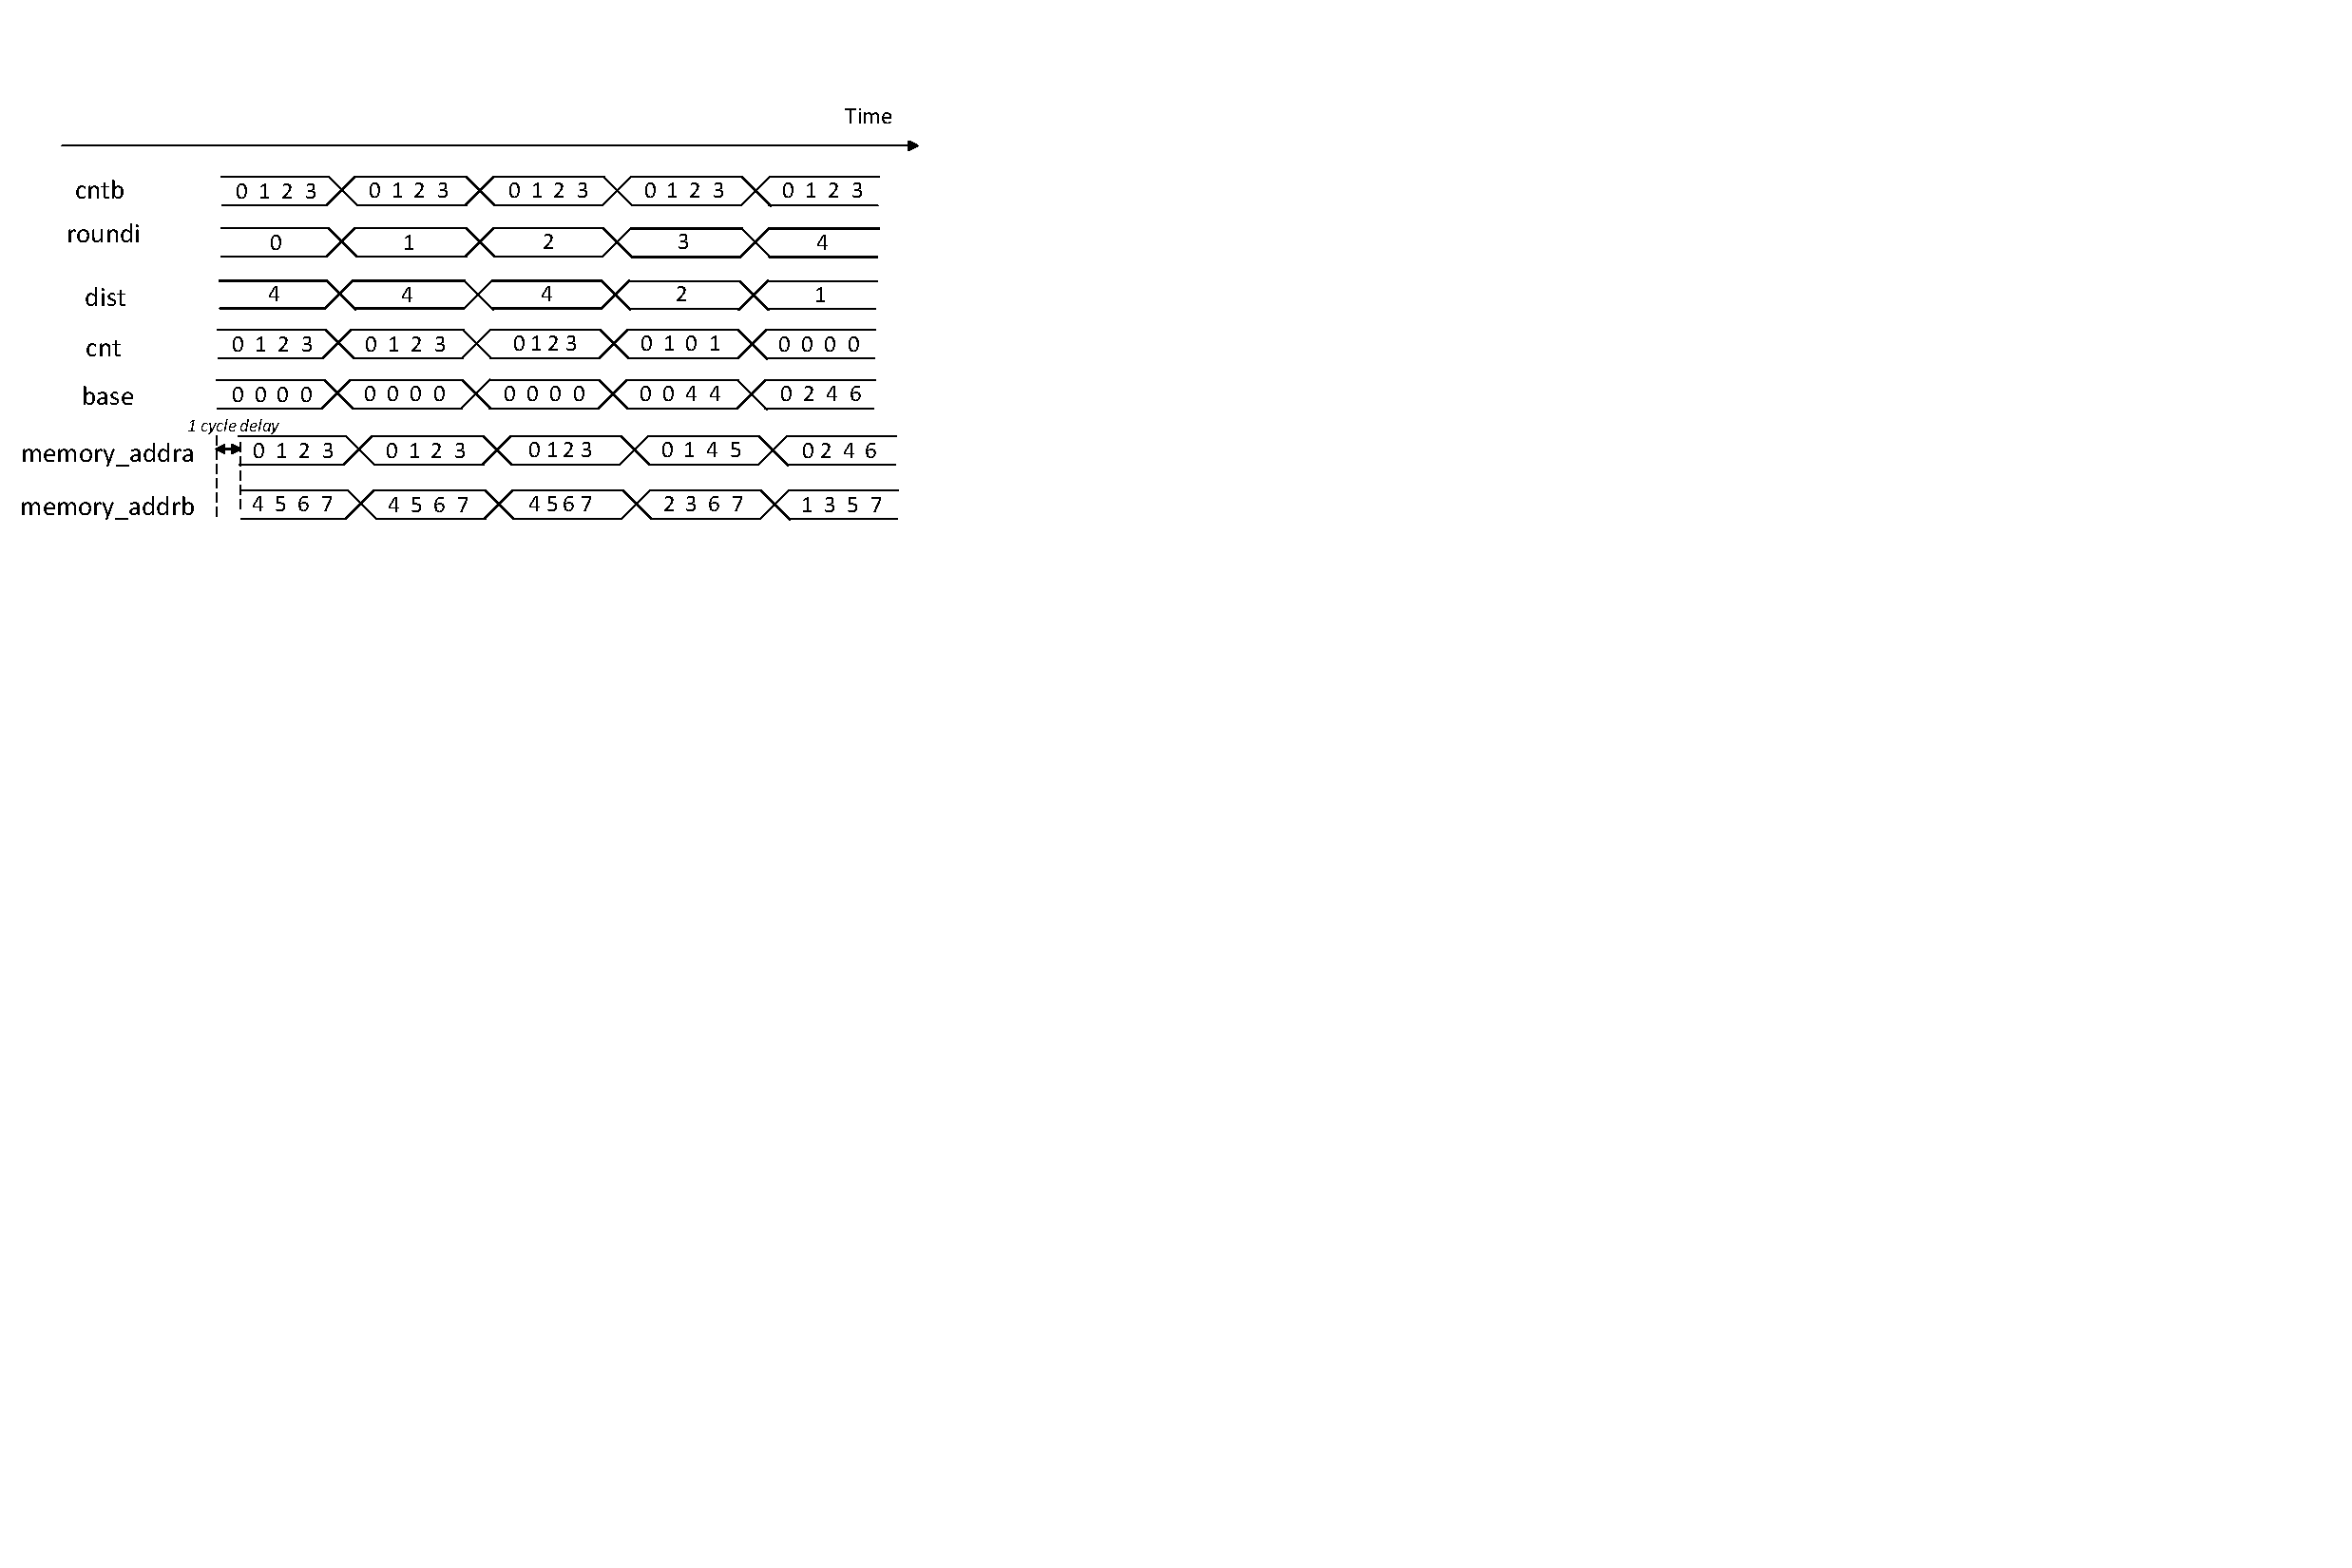
\includegraphics[width=\textwidth]{./fig/timing_diag.pdf}
\caption{Illustrative timing diagram for memory address generation in line with Alg.~\ref{alg:addrgen}($N=32, d=4$)}\label{fig:timing_diag}
\end{figure*}

\begin{figure*}[!tb]
\centering
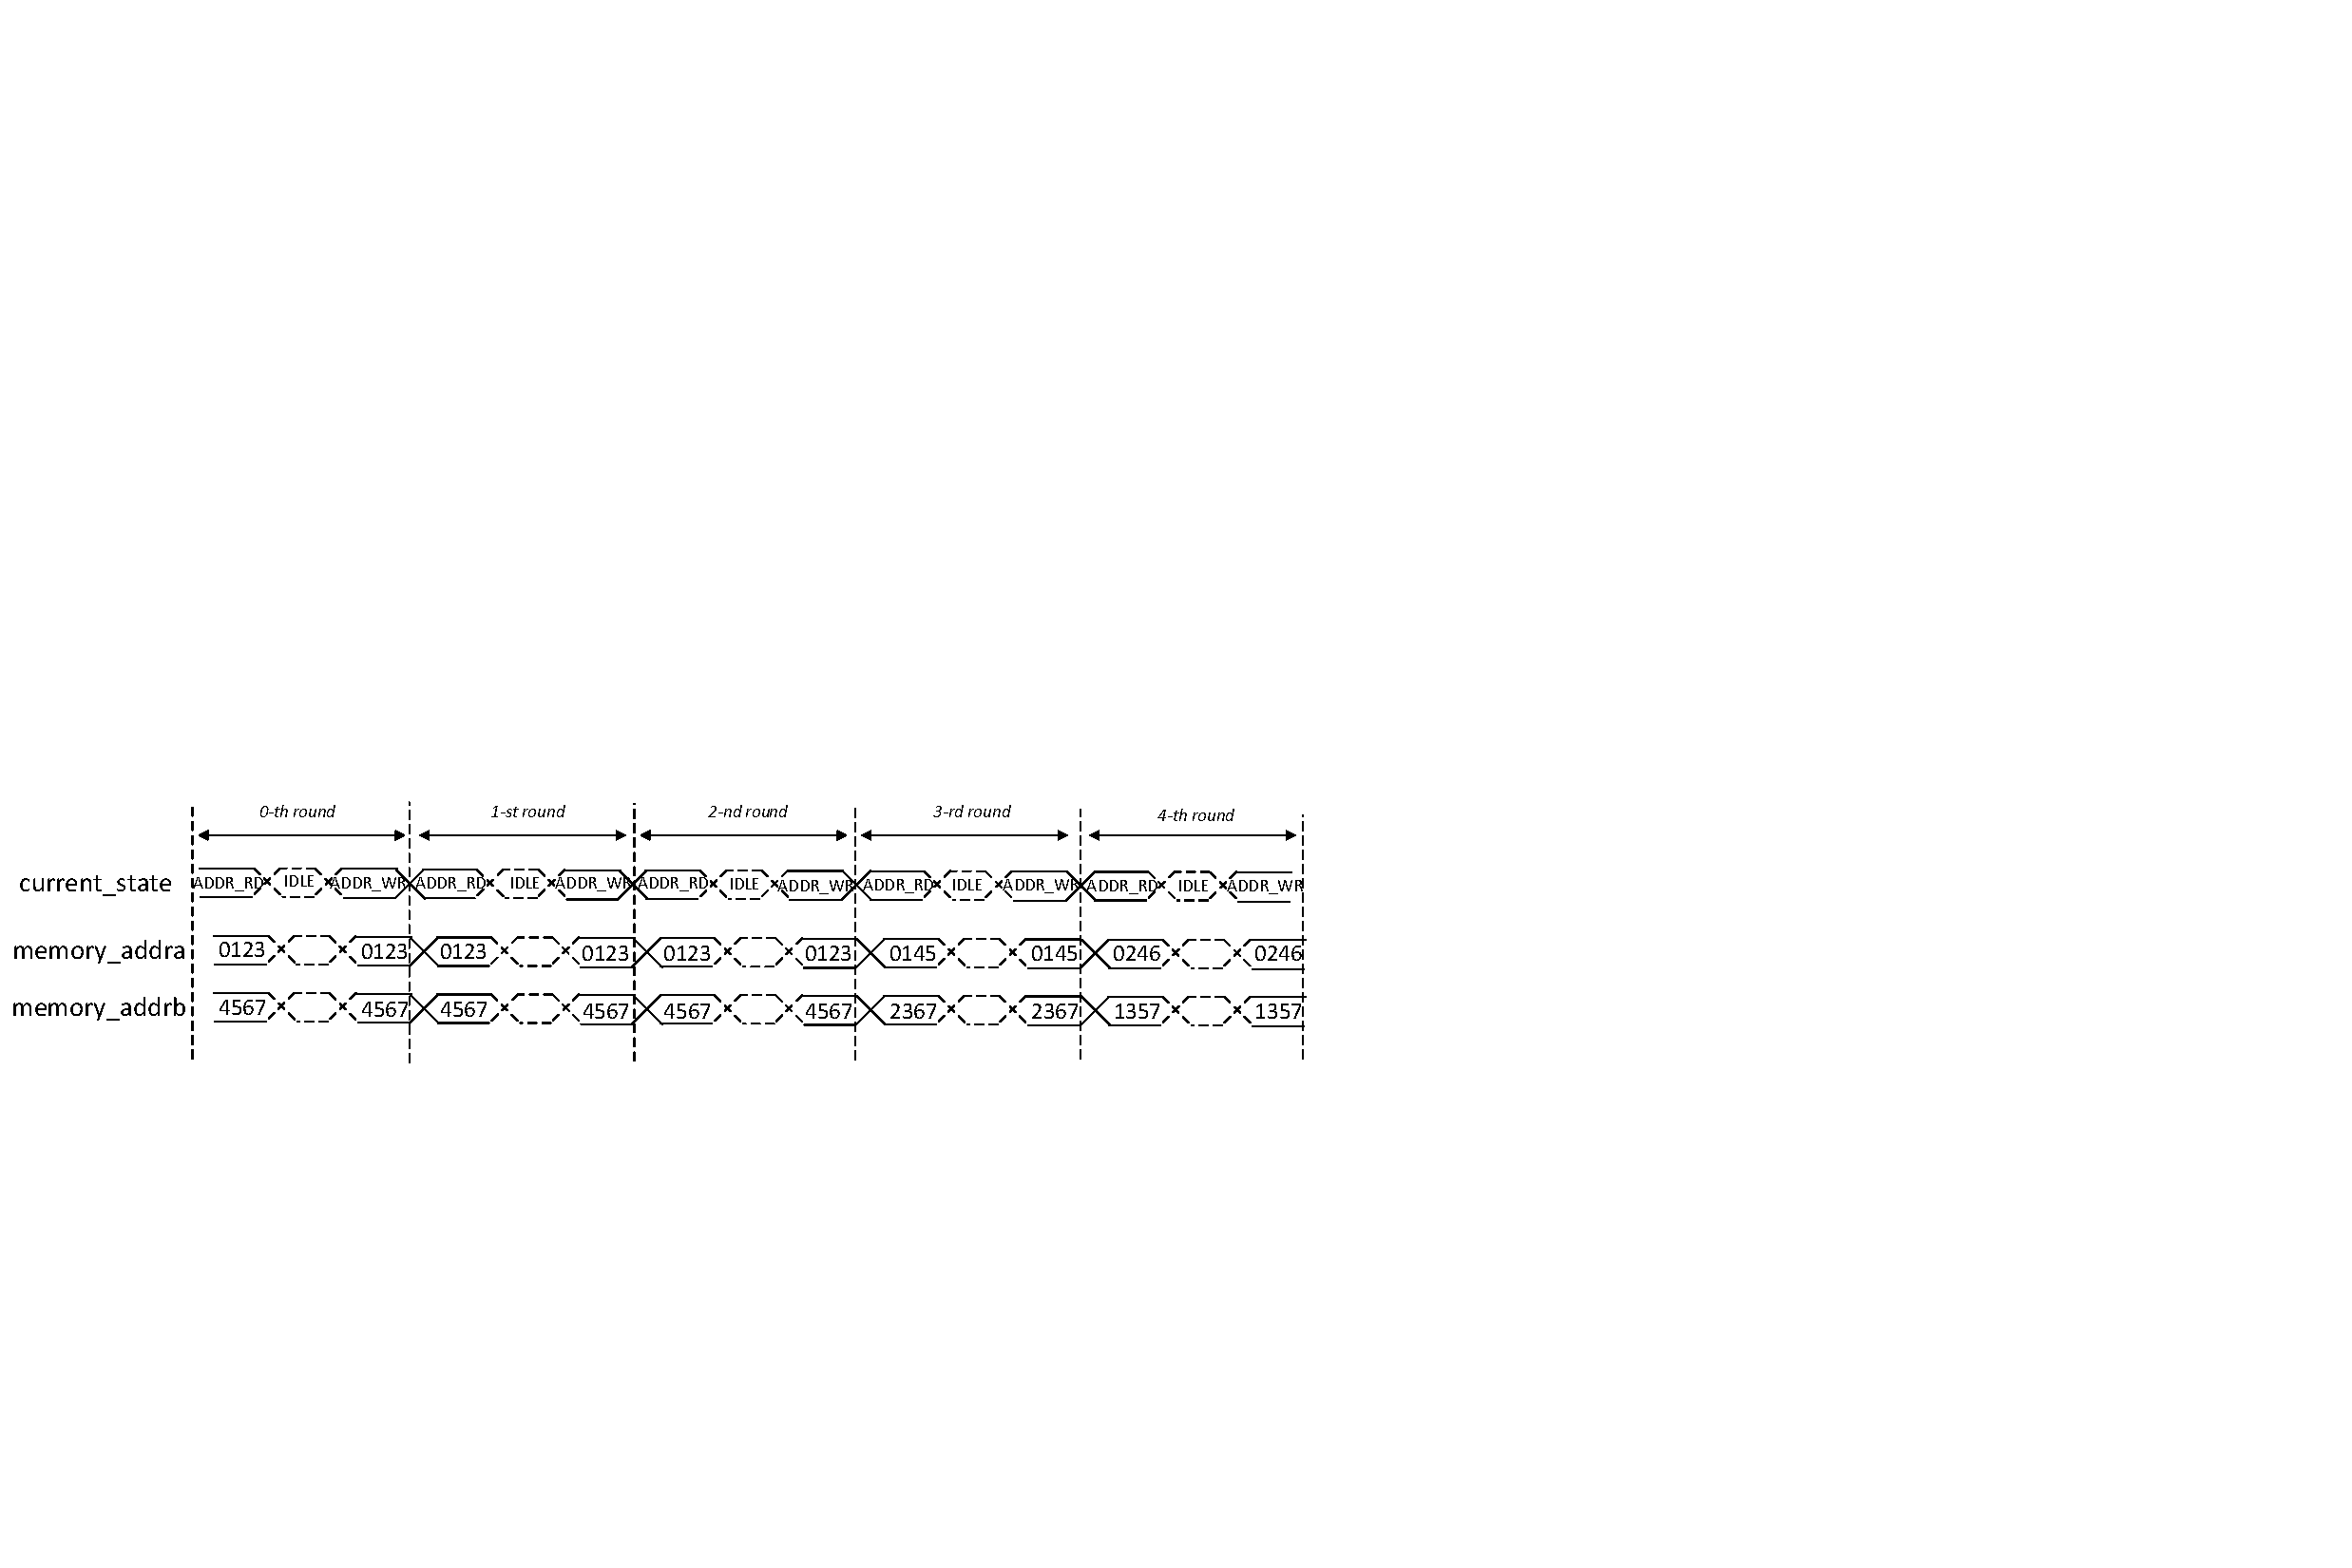
\includegraphics[width=\textwidth]{./fig/timing_diag2.pdf}
\caption{Top-level timing diagram for hypercube NTT in 5 rounds($N=32, d=4$)}\label{fig:timing_diag2}
\end{figure*}


\subsection{Implementation Experiments}

 \begin{table*}[!t]\centering
 \caption{Performance of the configurable hypercube NTT hardware for FHEW-like FHE schemes on Xilinx Artix-7 FPGA}
 \label{table:hypercube-ntt-result}
 \begin{minipage}{\textwidth}\centering
 \scalebox{0.8}{\begin{tabular}{lcccccc}
 \hline
 Instance   & \# of processors & freq & cycle & CLB/LUT/Reg &   memory & DSPs \\
 \hline
 \multirow{5}{*}{$N=1024,q\approx 2^{32}$} & 2 & 100 & 5120 & 451/2309/1756  & 3 & 30 \\
             &                                        4 & 100 & 2560 & 760/3581/2940 &   6 & 60 \\
             &                                        8 & {100} & 1280  & 1402/4238/5480 & 12  & 120 \\
             &                                        16 & 100 & 640 & 2174/10669/10591 & 24 & 240 \\
             &                                        32 & 100 & 430 & 3937/19250/18738 & 48 & 480 \\
             &                                        64 & 80 & 350 & 7835/39009/37060 & 96 & 960 \\
 \hline
  \hline
 \end{tabular}}
 \end{minipage}
 \vspace{0mm}
 \end{table*}


\textbf{Timing analysis} The main states we used are \texttt{ADDR\_RD} and \texttt{ADDR\_WR} which are used for memory read and memory write, respectively. If the delay of butterfly computation is longer than that of \texttt{ADDR\_RD}, then an auxillary state called \texttt{IDLE} is inserted in between because the node processor cannot write valid data back to memory until the butterfly unit outputs the NTT results. Precisely speaking, if $\frac{N}{2d}-T_{\texttt{ADDR\_RD}}+1<T_{\texttt{butterfly}}$, then \texttt{IDLE} with delay $T_{\texttt{IDLE}}=T_{\texttt{butterfly}}-\frac{N}{2d}+T_{\texttt{ADDR\_RD}}-1$ is required. The delay for the state \texttt{ADDR\_RD} and the state \texttt{ADDR\_WR} are $\frac{N}{2d}$ respectively, \textit{i.e.}, $T_{\texttt{ADDR\_RD}} = T_{\texttt{ADDR\_WR}}= \frac{N}{2d}$. In summary, the total delay for the hypercube NTT with $d$ processors is:
\[
    logN\cdot\left(\frac{N}{d}+max(T_{\texttt{IDLE}},0)\right )
\]

In our concrete experiment, $T_{\texttt{ADDR\_RD}}$ set to $1$ and $T_{\texttt{butterfly}}$ set to $27$. Therefore the total delay for the hypercube NTT is further simplified to $logN\cdot(\frac{N}{d}+max(27-\frac{N}{2d},0))$.


\textbf{Experimental data} The proposed design is implemented on Xilinx Zynq UltraScale+ ZCU106 evaluation board using Vivado 2018.1. The number of NTT points is set to 1024, a typical value used in FHE schemes. The number of NTT processors is configured to 2,4,8,16,32, and 64 to fully demonstrate the scalability of our hypercube NTT design. It is worth mentioning that our implementation follows the parameterized design approach, \textit{i.e.}, our NTT hardware can be customized and auto-generated on the fly from a script file by inputting core parameters of hypercube NTT, for example, $N$ and $d$. The experimental results are collected in Table.~\ref{table:hypercube-ntt-result}. As the parameter $d$ increases, the clock frequency is rather stable around $100$ MHz, which indicates the hypercube memory swapping strategy is successful to maintain a good critical path delay. 
If the number of processors is smaller than $32$, the cycle delay equals to $logN\cdot\frac{N}{d}$ and thus the increase of $d$ reduces significantly the cycle delay: for example, doubling $d$ suggests cycle delay reduced by half. As the number of processors gets even bigger ($\geq 32$), the \texttt{IDLE} state is inserted and the cycle delay equals to $logN\cdot(\frac{N}{2d}+27)$ for which the performance boost by increasing $d$ is rather marginal.  For this case, we can optimize the performance of butterfly computation (more concretely, modular reduction) to further improve it. However, we do not push the limit on this direction which is not the focus in this paper.


\section{System Integration on Xilinx MPSOC platform}
We also conduct FPGA experiment where the NTT module is implemented in PL logic and the FHEW software (written in C++) runs on ARM PS logic. The target hardware platform is Xilinx Versal VMK180 development board. Each NTT node processor (together with its internal block memory) is implemented as a AXI master device. NTT node processors communicate with each other for memory exchange through MUX interface. The content in internal block memory of the node processor is updated by the PS DDR memory through AXI DMA interface. It is worth noting that the block memory update is frequent: whenever an NTT computation is required, the block memory content must be refreshed. Typically, a single FHEW bootstrapping operation involves thousands of NTT computations. 


\begin{figure*}[!tb]
\centering
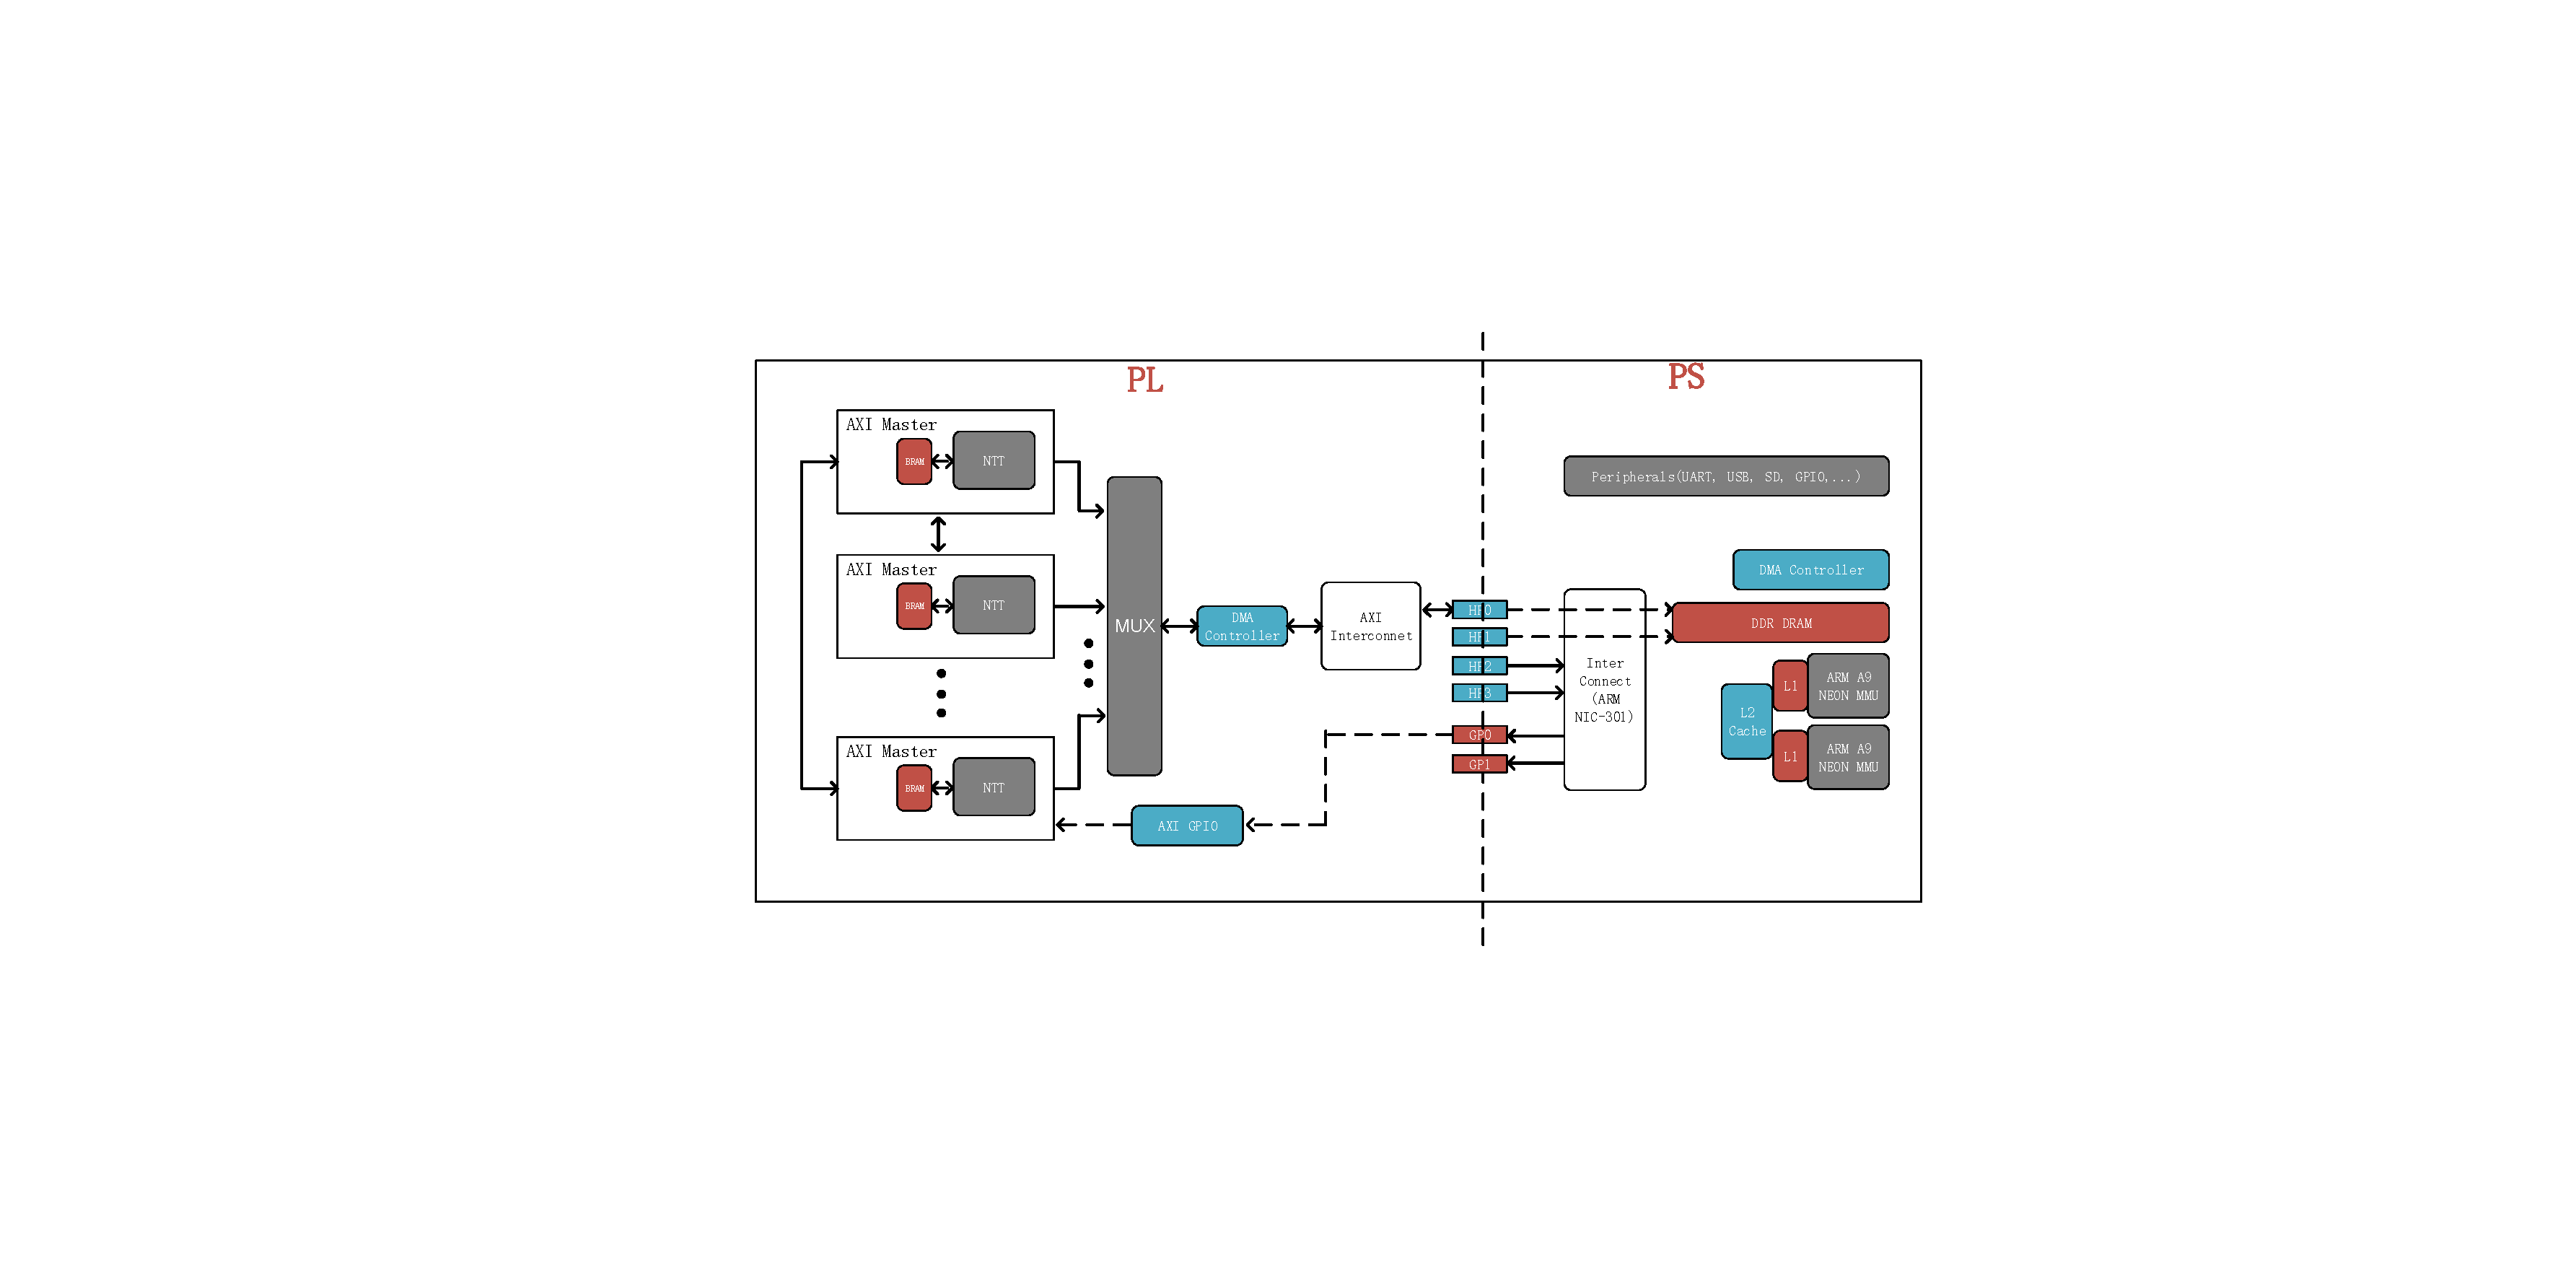
\includegraphics[width=\textwidth]{./fig/xilinx_mpsoc.pdf}
\caption{A software-hardware co-design for FHEW where the NTT module is implemented in PL logic and the software runs in PS logic}\label{fig:mpsoc}
\end{figure*}


\textbf{Performance}


\section{Conclusions}
% This paper presented a complete FPGA implementation of the ROLLO scheme using LRPC codes.
% It is the first hardware implementation of a rank-metric code based cryptosystem that supports varying security parameters. The efficiency of our design is achieved by a novel Gaussian elimination structure, a simplified implementation strategy for the rank support recovery algorithm, and a fast interleaved polynomial multiplier, among others. The proposed parameterized architectures, such as the Gaussian elimination and the polynomial multiplication, are not limited to instances used in ROLLO but also fully support other rank-code based schemes. For example, RQC applies the identical family of ideal codes to construct the public key and the ciphertext, therefore, the $\mathbb{F}_{2m}[z]$ arithmetic presented in this work can be directly reused as the underlying arithmetic; At the core of RQC key generation and data encryption algorithm, the generation of vectors over $\mathbb{F}_{2}$ with prescribed rank weight is demanding, and the parameterized Gaussian elimination systolic array can be adpated effortlessly for this task.

\bibliographystyle{alpha}
\bibliography{./reference}


\end{document}
